\documentclass[12pt,a3paper]{article}

%% ── Packages ──────────────────────────────────────────────────────────
\usepackage{amsmath,amssymb}
\usepackage{geometry}
\usepackage{enumitem}
\usepackage{titlesec}
\usepackage[hidelinks,colorlinks=true,linkcolor=blue!70!black]{hyperref}
\usepackage{xcolor}
\usepackage{fancyhdr}
\usepackage{tcolorbox}
\usepackage{multicol}
\usepackage{needspace}
\usepackage[strings]{underscore}
\usepackage{array,booktabs}
\usepackage{multirow}
\usepackage[table]{xcolor}
\usepackage{tikz}
\usepackage{listings}
\usepackage{makecell}
\usepackage{tabularx}
\usetikzlibrary{matrix}

\tcbuselibrary{listings}
\usetikzlibrary{shapes.multipart, positioning, calc, arrows.meta}



% Color definition for syntax highlighting
\definecolor{pbblue}{HTML}{005CC5}
\definecolor{pgreen}{HTML}{22863A}
\definecolor{pred}{HTML}{D73A49}
\definecolor{pcomment}{HTML}{6A737D}

\usetikzlibrary{shapes.geometric, positioning, arrows.meta, calc}
\usetikzlibrary{automata, positioning, arrows.meta}

\tcbuselibrary{skins,breakable}
\geometry{margin=2.5cm,headheight=20pt,top=3cm,bottom=3cm}

%% ── Colors ────────────────────────────────────────────────────────────
\definecolor{pblue}{RGB}{13,71,161}
\definecolor{dgray}{RGB}{66,66,66}
\definecolor{cA}{RGB}{183,28,28}
\definecolor{cB}{RGB}{1,87,155}
\definecolor{cC}{RGB}{27,94,32}
\definecolor{cD}{RGB}{106,27,154}
\definecolor{cE}{RGB}{230,81,0}
\definecolor{cF}{RGB}{0,96,100}
\definecolor{cG}{RGB}{136,14,79}
\definecolor{cH}{RGB}{0,77,64}
\definecolor{cI}{RGB}{62,39,35}


\definecolor{pbbblue}{HTML}{005CC5}
\definecolor{pcomment}{HTML}{6A737D}
\definecolor{pstring}{HTML}{032F62}
\definecolor{glassybg}{RGB}{245, 246, 250} % Very light, soft background
%% ── C listing style ───────────────────────────────────────────────────
\lstdefinestyle{Cstyle}{
  language=C,
  basicstyle=\small\ttfamily,
  keywordstyle=\bfseries\color{pbbblue},
  commentstyle=\itshape\color{pcomment},
  stringstyle=\color{pstring},
  numberstyle=\tiny\color{gray},
  numbers=left,
  stepnumber=1,
  numbersep=10pt,
  breaklines=true,
  frame=l,                      % Shudhu left e border thakbe
  framesep=4.5mm,
  framexleftmargin=2.5mm,
  rulecolor=\color{pblue!50},   % Left border er color
  backgroundcolor=\color{glassybg}, % Soft background
  fillcolor=\color{white},
  aboveskip=15pt,
  belowskip=15pt,
  showstringspaces=false,
  tabsize=4
}

\lstset{style=Cstyle}

% % Modern Transparent Box Style
% \newtcblisting{myCcode}[1][]{
%   listing only,
%   listing options={
%     language=C,
%     basicstyle=\small\ttfamily,
%     keywordstyle=\bfseries\color{pbblue},
%     commentstyle=\itshape\color{pcomment},
%     stringstyle=\color{pred},
%     numberstyle=\tiny\color{gray},
%     numbers=left,
%     stepnumber=1,
%     numbersep=10pt,
%     breaklines=true,
%     showstringspaces=false,
%     tabsize=4,
%   },
%   enhanced,
%   colback=white,           % Background color (white)
%   opacityback=0.5,         % Transparency of background (0.0 to 1.0)
%   colframe=gray!30,        % Border color
%   opacityframe=0.7,        % Transparency of border
%   arc=4mm,                 % Rounded corners
%   boxrule=1pt,             % Border thickness
%   drop fuzzy shadow=gray!40, % Soft shadow for modern look
%   left=5pt,
%   right=5pt,
%   top=5pt,
%   bottom=5pt,
%   #1
% }

%% ── Section headings ──────────────────────────────────────────────────
\titleformat{\section}{\large\bfseries\color{pblue}}{}{0em}{}[\titlerule]
\titleformat{\subsection}{\normalsize\bfseries}{}{0em}{}



%% ── Header / Footer ───────────────────────────────────────────────────
\pagestyle{fancy}\fancyhf{}
\renewcommand{\headrulewidth}{0.5pt}
\fancyhead[L]{\small\textcolor{pblue}{\textbf{BUET $|$ CSE 101 Question Bank}}}
\fancyhead[R]{\small\textcolor{dgray}{\textit{\nouppercase{\leftmark}}}}
\fancyfoot[C]{\small\thepage}


% Custom column type for centering text with a fixed width
\newcolumntype{C}[1]{>{\centering\arraybackslash}p{#1}}


%% ── Utility macros ────────────────────────────────────────────────────
\newcommand{\yr}[1]{\hfill\textcolor{gray}{\small\textbf{[#1]}}}
\newcommand{\mk}[1]{\textcolor{orange!70!black}{\small\textbf{(#1 marks)}}}
\newcommand{\variant}[1]{\par\vspace{1pt}\textcolor{blue!50!black}%
  {\footnotesize\textit{$\hookrightarrow$ Similar: #1}}}
\newcommand{\visualnote}[1]{\par\vspace{2pt}%
  {\footnotesize\textcolor{cG}{\textit{\textbf{[Visual:} #1\textbf{]}}}}}

%% ── Subtopic heading macro ────────────────────────────────────────────
\newcommand{\subtopic}[2]{%
  \vspace{10pt}
  \noindent\begin{tcolorbox}[colback=#1!8,colframe=#1,boxrule=0.6pt,arc=4pt,
    left=6pt,right=6pt,top=4pt,bottom=4pt]
    \small\bfseries\textcolor{#1}{#2}
  \end{tcolorbox}
  \vspace{2pt}
}

%% ── Section divider page ──────────────────────────────────────────────
\newcommand{\secdivider}[4]{%
  \newpage\thispagestyle{empty}%
  \vspace*{\fill}%
  \begin{tcolorbox}[enhanced,colback=#4!7,colframe=#3,boxrule=1.5pt,arc=8pt,
    left=20pt,right=20pt,top=22pt,bottom=22pt,
    shadow={3pt}{-3pt}{0pt}{black!15}]
    \centering
    {\large\textcolor{gray}{\textbf{BUET $\cdot$ CSE 101 $\cdot$ Structured Programming}}}\\[8pt]
    {\fontsize{26}{32}\selectfont\bfseries\textcolor{#3}{#1}}\\[6pt]
    {\fontsize{15}{19}\selectfont\textcolor{dgray}{#2}}\\[12pt]
    \textcolor{#3!60}{\rule{0.5\textwidth}{0.5pt}}\\[6pt]
    {\small\textcolor{gray}{#2}}
  \end{tcolorbox}%
  \vspace*{\fill}\newpage%
}


%% ── List styles ───────────────────────────────────────────────────────
\setlist[enumerate,1]{label=\textbf{Q\arabic*.},leftmargin=*,itemsep=14pt,parsep=2pt}
\setlist[enumerate,2]{label=(\alph*),leftmargin=2em,itemsep=3pt}
\setlist[enumerate,3]{label=(\roman*),leftmargin=2.5em,itemsep=2pt}
\begin{document}

%% ══════════════════════════════════════════════════════════════════════
%%  COVER PAGE
%% ══════════════════════════════════════════════════════════════════════
\thispagestyle{empty}
\begin{tcolorbox}[enhanced,colback=pblue!5,colframe=pblue,boxrule=1.5pt,arc=6pt,
  top=28pt,bottom=28pt,left=22pt,right=22pt,
  shadow={4pt}{-4pt}{0pt}{black!20}]
  \centering

    
\includegraphics[height=2.5cm]{images/buet_logo.png}\\[8pt]

  {\Large\bfseries\textcolor{pblue}{Bangladesh University of Engineering and Technology}}\\[4pt]
  {\normalsize\textcolor{dgray}{Department of Computer Science \& Engineering}}\\[18pt]
  \textcolor{pblue}{\rule{\textwidth}{1pt}}\\[14pt]
  {\fontsize{22}{28}\selectfont\bfseries\textcolor{pblue}{Structured Programming Question Bank}}\\[8pt]
  {\fontsize{14}{18}\selectfont\textcolor{dgray}{CSE 101 $\cdot$ Structured Programming Language}}\\[4pt]
  \textcolor{pblue}{\rule{\textwidth}{0.5pt}}\\[14pt]
  {\small\textcolor{dgray}{Year Coverage: 2003--04 to 2024--25\\Topics:\;Data Types \& Operators, Control Structures, Functions,\\
  Arrays \& Strings, Recursion, Pointers, Structures \& Unions,\\
  File I/O, Bitwise Operations, Preprocessors, Error Handling}}\\[16pt]
    {\small\bfseries\textcolor{dgray}{Authors \& Contributors}}\\[6pt]
    \begin{tabular}{rl}
      \textcolor{dgray}{\textbf{Md Ratul Hasan}} \textcolor{dgray}{\small(2405009)} & --- Question Curation \& Organisation\\
      & --- \LaTeX\ Typesetting\\[3pt]
      \textbf{NotebookLM} & --- Research \& Extraction\\[3pt]
      \textbf{Claude AI}  & --- \LaTeX\ Typesetting\\[3pt]
      \textbf{Gemini}     & --- Diagram Generation\\[3pt]
    \end{tabular}
\end{tcolorbox}
\newpage

%% ══════════════════════════════════════════════════════════════════════
%%  TABLE OF CONTENTS
%% ══════════════════════════════════════════════════════════════════════
\thispagestyle{fancy}\markboth{Table of Contents}{}
\begin{center}
  {\LARGE\bfseries\textcolor{pblue}{Table of Contents}}\\[6pt]
  \textcolor{pblue}{\rule{0.6\textwidth}{0.8pt}}
\end{center}
\vspace{6pt}

%% Part I
\begin{tcolorbox}[breakable,colback=cA!5,colframe=cA,boxrule=1pt,arc=5pt,
  left=8pt,right=8pt,top=8pt,bottom=8pt,before skip=4pt]
  {\large\bfseries\textcolor{cA}{Part I --- Fundamentals}}\\[5pt]
  \textcolor{cA!40}{\rule{\textwidth}{0.4pt}}\\[3pt]
  \small\begin{itemize}[leftmargin=1.2em,itemsep=1pt,label={\textcolor{cA}{$\triangleright$}}]
    \item \hyperref[sec:S1]{\textbf{S1.} Data Types, Variables \& Operators}
      \begin{itemize}[leftmargin=1.5em,itemsep=0pt,label={\textcolor{cA}{$\cdot$}}]
        \item \hyperref[sub:s1-datatypes]{Data Types \& Variables}
        \item \hyperref[sub:s1-operators]{Operators, Expressions \& Type-Casting}
      \end{itemize}
    \item \hyperref[sec:S2]{\textbf{S2.} Control Structures}
      \begin{itemize}[leftmargin=1.5em,itemsep=0pt,label={\textcolor{cA}{$\cdot$}}]
        \item \hyperref[sub:s2-ifelse]{if-else \& switch-case}
        \item \hyperref[sub:s2-loops]{Loops (while, do-while, for)}
        \item \hyperref[sub:s2-nested]{Nested Control, break \& continue}
        \item \hyperref[sub:s2-goto]{\texttt{goto} Statement}
      \end{itemize}
  \end{itemize}
\end{tcolorbox}

%% Part II
\begin{tcolorbox}[breakable,colback=cB!5,colframe=cB,boxrule=1pt,arc=5pt,
  left=8pt,right=8pt,top=8pt,bottom=8pt,before skip=4pt]
  {\large\bfseries\textcolor{cB}{Part II --- Functions \& Arrays}}\\[5pt]
  \textcolor{cB!40}{\rule{\textwidth}{0.4pt}}\\[3pt]
  \small\begin{itemize}[leftmargin=1.2em,itemsep=1pt,label={\textcolor{cB}{$\triangleright$}}]
    \item \hyperref[sec:S3]{\textbf{S3.} Functions}
      \begin{itemize}[leftmargin=1.5em,itemsep=0pt,label={\textcolor{cB}{$\cdot$}}]
        \item \hyperref[sub:s3-funcbasics]{Function Basics \& Parameter Passing}
        \item \hyperref[sub:s3-recursion]{Recursion}
      \end{itemize}
    \item \hyperref[sec:S4]{\textbf{S4.} Arrays \& Strings}
      \begin{itemize}[leftmargin=1.5em,itemsep=0pt,label={\textcolor{cB}{$\cdot$}}]
        \item \hyperref[sub:s4-1darray]{One-Dimensional Arrays: Searching \& Sorting}
        \item \hyperref[sub:s4-strings]{Character \& String Operations}
        \item \hyperref[sub:s4-2darray]{Multi-Dimensional Arrays \& Matrix Operations}
      \end{itemize}
  \end{itemize}
\end{tcolorbox}

%% Part III
\begin{tcolorbox}[breakable,colback=cC!5,colframe=cC,boxrule=1pt,arc=5pt,
  left=8pt,right=8pt,top=8pt,bottom=8pt,before skip=4pt]
  {\large\bfseries\textcolor{cC}{Part III --- Pointers \& User-Defined Types}}\\[5pt]
  \textcolor{cC!40}{\rule{\textwidth}{0.4pt}}\\[3pt]
  \small\begin{itemize}[leftmargin=1.2em,itemsep=1pt,label={\textcolor{cC}{$\triangleright$}}]
    \item \hyperref[sec:S5]{\textbf{S5.} Pointers}
      \begin{itemize}[leftmargin=1.5em,itemsep=0pt,label={\textcolor{cC}{$\cdot$}}]
        \item \hyperref[sub:s5-ptrbasics]{Pointer Basics}
        \item \hyperref[sub:s5-ptradv]{Pointers to Arrays, Strings, Structs \& Functions}
        \item \hyperref[sub:s5-dynmem]{Dynamic Memory Allocation}
      \end{itemize}
    \item \hyperref[sec:S6]{\textbf{S6.} User-Defined Data Types}
      \begin{itemize}[leftmargin=1.5em,itemsep=0pt,label={\textcolor{cC}{$\cdot$}}]
        \item \hyperref[sub:s6-struct]{Structures}
        \item \hyperref[sub:s6-union]{Unions, Bit-fields \& Enumerations}
      \end{itemize}
  \end{itemize}
\end{tcolorbox}

%% Part IV
\begin{tcolorbox}[breakable,colback=cD!5,colframe=cD,boxrule=1pt,arc=5pt,
  left=8pt,right=8pt,top=8pt,bottom=8pt,before skip=4pt]
  {\large\bfseries\textcolor{cD}{Part IV --- I/O, Bitwise, Preprocessors \& Miscellaneous}}\\[5pt]
  \textcolor{cD!40}{\rule{\textwidth}{0.4pt}}\\[3pt]
  \small\begin{itemize}[leftmargin=1.2em,itemsep=1pt,label={\textcolor{cD}{$\triangleright$}}]
    \item \hyperref[sec:S7]{\textbf{S7.} Input/Output}
      \begin{itemize}[leftmargin=1.5em,itemsep=0pt,label={\textcolor{cD}{$\cdot$}}]
        \item \hyperref[sub:s7-consoleio]{Console \& Formatted I/O}
        \item \hyperref[sub:s7-fileio]{File I/O \& Command Line Arguments}
      \end{itemize}
    \item \hyperref[sec:S8]{\textbf{S8.} Bitwise Operations}
      \begin{itemize}[leftmargin=1.5em,itemsep=0pt,label={\textcolor{cD}{$\cdot$}}]
        \item \hyperref[sub:s8-bitwise]{Bitwise Operators \& Applications}
      \end{itemize}
    \item \hyperref[sec:S9]{\textbf{S9.} Preprocessors, Var-Arg \& Error Handling}
      \begin{itemize}[leftmargin=1.5em,itemsep=0pt,label={\textcolor{cD}{$\cdot$}}]
        \item \hyperref[sub:s9-preproc]{Header Files \& Preprocessors}
        \item \hyperref[sub:s9-vararg]{Variable Argument Functions}
        \item \hyperref[sub:s9-error]{Error Handling}
      \end{itemize}
  \end{itemize}
\end{tcolorbox}

%% Part V
\begin{tcolorbox}[breakable,colback=cE!5,colframe=cE,boxrule=1pt,arc=5pt,
  left=8pt,right=8pt,top=8pt,bottom=8pt,before skip=4pt]
  {\large\bfseries\textcolor{cE}{Part V --- Data Structures}}\\[5pt]
  \textcolor{cE!40}{\rule{\textwidth}{0.4pt}}\\[3pt]
  \small\begin{itemize}[leftmargin=1.2em,itemsep=1pt,label={\textcolor{cE}{$\triangleright$}}]
    \item \hyperref[sec:S10]{\textbf{S10.} Abstract Data Structures}
      \begin{itemize}[leftmargin=1.5em,itemsep=0pt,label={\textcolor{cE}{$\cdot$}}]
        \item \hyperref[sub:s10-linkedlist]{Linked Lists}
        \item \hyperref[sub:s10-stackqueue]{Stacks \& Queues}
        \item \hyperref[sub:s10-bst]{Binary Search Trees}
      \end{itemize}
  \end{itemize}
\end{tcolorbox}

\newpage

%% ══════════════════════════════════════════════════════════════════════
%%  PART I — FUNDAMENTALS
%% ══════════════════════════════════════════════════════════════════════
\secdivider{Part I}{Fundamentals}{cA}{cA}

%% ── S1: Data Types, Variables & Operators ─────────────────────────────
\section{S1 --- Data Types, Variables \& Operators}
\label{sec:S1}
\markboth{S1 --- Data Types, Variables \& Operators}{}

%%──────────────────────────────────────────────────────────────────────
\subtopic{cA}{Data Types \& Variables}
\label{sub:s1-datatypes}

\begin{enumerate}

%% Q9 — 2023-24
\item You want to store the vaccination records of diphtheria, typhoid, cholera, polio, tetanus, and measles applied to a child (each vaccination is either given or not). Which data type will be optimal for storing this information? Justify your answer.
\mk{4} \yr{CSE 101 | L-1/T-1 | 2024--25, 2023--24}

%% Q10 — 2003-04
\item Write down the desirable characteristics of a good program. Define escape sequences with examples.
\mk{9} \yr{CSE 101 | L-1/T-1 | 2020--21}

%% Q27 — 2020-21
\item What is meant by a \textit{token}? Describe why the distinction between a reserved word and a keyword is significant in natural language but not in programming language.
\mk{7} \yr{CSE 101 | L-1/T-1 | 2020--21}

\item How is a static local variable declared? Explain with an example how a static local variable differs from a regular local variable.
\mk{10} \yr{CSE 101 | L-1/T-1 | 2018--19}

%% Q26 — 2020-21
\item Write a C program that will display the details of the program's running configuration environment on the monitor screen.
\mk{7} \yr{CSE 105 | L-1/T-2 | 2013--14}

%% Q25 — 2018-19
\item Consider the following code fragment:
 
\begin{lstlisting}
int i = 'c';
\end{lstlisting}
Are we allowed to assign a character constant to an \texttt{int} variable? First answer yes or no, then explain your reasoning.
\mk{5} \yr{CSE 105 | L-1/T-2 | 2012--13}

%% Q24 — 2013-14
\item What is an escape sequence? What is the purpose of using escape sequences in C programming?
\mk{5} \yr{CSE 105 | L-1/T-2 | 2011--12}

%% Q22 — 2011-12
\item Write down some characteristics that are to be followed when writing a good computer program.
\mk{6} \yr{CSE 105 | L-1/T-2 | 2011--12}

%% Q23 — 2012-13
\item Write some differences between \texttt{signed} and \texttt{unsigned} data types. Can these qualifiers be applied to \texttt{double} or \texttt{float}?
\mk{5} \yr{CSE 105 | L-1/T-2 | 2010--11}

%% Q19 — 2010-11
\item Write a simple program to find the size of different basic data types in C.
\mk{5} \yr{CSE 105 | L-1/T-2 | 2010--11}

%% Q20 — 2010-11
\item Write short notes on local, global, and static variables. What are the features of static local and static global variables?
\mk{10} \yr{CSE 105 | L-1/T-2 | 2010--11}

%% Q21 — 2011-12
\item What will be the output of the following program? Explain your answer.
 
\begin{lstlisting}
#include <stdio.h>
int main() {
    short int nl = 130;
    char ch = 'a';
    printf("\n nl's value is: %d", nl);
    printf("\n ch's value is: %d", ch);
    nl += ch + 230;
    ch += nl + 470;
    printf("\n nl's value is: %d", nl);
    printf("\n ch's value is: %c", ch);
    printf("\n");
    return 0;
}
\end{lstlisting}
\mk{10} \yr{CSE 101 | L-1/T-2 | 2009--10}

%% Q16 — 2009-10
\item Which of the following variable declarations is right or wrong, and why?
\begin{lstlisting}
char ch = 256;
int _;
int long il;
char [25]name;
char *cp = 'z';
const int n;
long l;
double average.cgpa;
long float lf;
short char shortch;
\end{lstlisting}
\mk{15} \yr{CSE 101 | L-1/T-2 | 2009--10}

%% Q17 — 2009-10
\item When you want to manipulate a variable in a program by several functions, you can either (a) define the variable as a global variable with functions having no parameters and \texttt{void} return type, or (b) define the variable as a local variable with functions having appropriate parameters and return types. Write about the pros and cons of each approach.
\mk{10} \yr{CSE 101 | L-1/T-2 | 2009--10}

%% Q18 — 2010-11
\item With appropriate examples, describe different types of storage class specifications used in a C program.
\mk{12} \yr{CSE 101 | L-1/T-2 | 2008--09}

%% Q13 — 2005-06
\item Present a table showing the range and size of all primitive datatypes in C which can be used to store non-fractional numeric values.
\mk{10} \yr{CSE 105 | L-1/T-2 | 2007--08}

%% Q12 — 2008-09
\item What do you mean by the scope of an identifier? Discuss the scopes for a global variable.
\mk{7} \yr{CSE 105 | L-1/T-2 | 2005--06}

%% Q14 — 2005-06
\item Discuss different types of storage class specifiers.
\mk{10} \yr{CSE 105 | L-1/T-2 | 2005--06}

%% Q15 — 2009-10
\item We know that $5 = (101)_2$ and $7 = (111)_2$, while $10 = (1010)_2$ and $6 = (110)_2$. It is interesting to see that in the binary representation of an odd number the LSB (least significant, i.e.\ rightmost bit) is 1, and for an even number it is 0. Prove that this holds for any odd or even number.
\mk{12} \yr{CSE 101N | L-1/T-1 | 2003--04}

%% Q13 — 2003-04
\item An integer (2 bytes) has the value 20 in its low byte and 17 in its high byte. What is the value of the integer in decimal and hexadecimal?
\mk{6} \yr{CSE 101N | L-1/T-1 | 2003--04}

%% Q11 — 2007-08
\end{enumerate}

%%──────────────────────────────────────────────────────────────────────
\subtopic{cA}{Operators, Expressions \& Type-Casting}
\label{sub:s1-operators}

\begin{enumerate}

\item Write the equivalent expression of the followings without using any relational or logical operator:
\begin{lstlisting}
int a, b, c, d;
scanf("%d%d%d%d", &a, &b, &c, &d);
if(a >= b && c >= d)
    printf("Hi");
else
    printf("Bye");
\end{lstlisting}
\mk{5} \yr{CSE 101 | L-1/T-1 | 2024--25}


%% Q9 — 2022-23
\item Suppose you are given an integer \texttt{n} and a digit \texttt{d}. Build another integer \texttt{r} where \texttt{n} is reversed first and then \texttt{d} is inserted in front of it. For example, if \texttt{n = 532} and \texttt{d = 8}, then \texttt{r = 8235}. Write the complete C program.
\mk{10} \yr{CSE 101 | L-1/T-1 | 2022--23}

%% Q10 — 2022-23
\item Determine the output of the following C code segment:
\begin{lstlisting}
int x=20, y=10, z=0;
int a = x && !y || z;
int b = x++ * --y + !z;
printf("%d %d\n", a, b);
\end{lstlisting}
\mk{5} \yr{CSE 101 | L-1/T-1 | 2022--23}

%% Q11 — 2022-23
\item Write down the following three functions with the specified tasks. Assume that always a negative value will be supplied in parameter \texttt{x}. You are \textbf{not} allowed to use any branching or repetition statements.
\begin{enumerate}
  \item \texttt{int truncate(float x)} --- discards the fractional part and returns the integer.
  \item \texttt{int rounding(float x)} --- returns the nearest integer; in case of a tie, returns the larger one.
  \item \texttt{int ceiling(float x)} --- returns the smallest integer not less than \texttt{x}.
\end{enumerate}
\mk{15} \yr{CSE 101 | L-1/T-1 | 2022--23}

%% Q12 — 2003-04
\item Write two functions that return the ceiling and floor of a fractional number up to $n$ decimal places. The functions \texttt{ceiling} and \texttt{floor} return the nearest fractional numbers with $n$ decimal places greater than or equal to, and smaller than or equal to, the argument respectively. The use of any built-in function is not allowed.
\mk{10} \yr{CSE 101 | L-1/T-1 | 2021--22}

\item Consider the following program codes:
 
\begin{lstlisting}
int i = 8, j = 5, k;
float x = 0.005, y = -0.01;
char c = 'c', d = 'd';
k = (i - 3 * j) % (c + 2 * d) / (x - y);
\end{lstlisting}
Rewrite the last line using explicit type casting to avoid any error or warning. Evaluate the expression to find the value of \texttt{k}. How many times does type auto-conversion take place while evaluating the equation?
\mk{9} \yr{CSE 101 | L-1/T-1 | 2020--21}

%% Q32 — 2021-22
\item Suppose you are given an integer \texttt{n} and a digit \texttt{d}. Write a program to build another integer \texttt{r} where \texttt{d} is inserted in front of \texttt{n}. For example, if \texttt{n = 532} and \texttt{d = 8}, then \texttt{r} will be 8532.
\mk{10} \yr{CSE 101 | L-1/T-1 | 2019--20}

%% Q30 — 2019-20
\item Write the following two functions (assume a negative value will always be supplied):
\begin{enumerate}
  \item \texttt{int truncate(float x)} --- discards the fractional part and returns the integer.
  \item \texttt{int rounding(float x)} --- returns the nearest integer (in case of tie, returns the larger one).
  \item \texttt{int ceiling(float x)} --- returns the smallest integer not less than \texttt{x}.
\end{enumerate}
You are not allowed to use any branching or repetition statements.
\mk{15} \yr{CSE 101 | L-1/T-1 | 2019--20}

%% Q31 — 2020-21
\item What will be the output of the following program, if the input is 0?
 
\begin{lstlisting}
#include <stdio.h>
int main() {
    int i;
    scanf("%d", &i);
    if (++i) {
        int i = 50;
        printf("%d\n", i++);
    }
    printf("%d\n", i);
    return 0;
}
\end{lstlisting}
\mk{5} \yr{CSE 101 | L-1/T-1 | 2018--19}

%% Q29 — 2019-20
\item Is the following code fragment valid? What will be the output if so? State your reason.
 
\begin{lstlisting}
int a = 2, b = 5, c;
c = a +++ b;
printf("%d, %d, %d", a, b, c);
\end{lstlisting}
\mk{5} \yr{CSE 101 | L-1/T-1 | 2015--16}

%% Q26 — 2015-16 [Backlog]
\item Write a program that takes an English uppercase letter as input and prints the letter two positions after it in the alphabet in lowercase. For example, if the user enters \texttt{D} the output is \texttt{f}; if the input is \texttt{Z} the output is \texttt{b}. You are not allowed to use \texttt{if-else}, \texttt{switch-case}, or the ternary operator.
\mk{10} \yr{CSE 101 | L-1/T-1 | 2015--16}

%% Q27 — 2015-16
\item Suppose you are working with an integer (4 bytes, 32 bits). How can you find the value of the rightmost byte (8 bits) without using any bitwise operator?
\mk{5} \yr{CSE 101 | L-1/T-1 | 2015--16}

%% Q28 — 2018-19
\item State whether the following relational expressions are true or false:
\begin{enumerate}
  \item \texttt{'A' - 'Z' == 'a' - 'z'}
  \item \texttt{'0' == 0}
  \item \texttt{(x > 0) \&\& (x <= 0)}
  \item \texttt{\textasciitilde(x (\textasciitilde x)) == 0}
\end{enumerate}
\mk{6} \yr{CSE 105 | L-1/T-2 | 2014--15}

%% Q23 — 2014-15
\item The modulus operator (\texttt{\%}) finds the remainder when integer \texttt{x} is divided by integer \texttt{y}. Show how to find the remainder without using the modulus operator (you may use any other mathematical operators as many times as needed).
\mk{6} \yr{CSE 105 | L-1/T-2 | 2014--15}

%% Q24 — 2014-15
\item You are given an unsigned integer as input. Using its bit pattern to represent a floating-point number, produce the corresponding floating-point value. Write the necessary code and explain.
\mk{5} \yr{CSE 105 | L-1/T-2 | 2014--15}

%% Q25 — 2015-16 [Backlog]
\item Assume \texttt{int x} has been declared and initialized to an unknown value. For each of the following, indicate if the expression \textbf{always} evaluates to true, or if it could \textbf{sometimes} be false (and if so, give a counterexample value of \texttt{x}):
\begin{enumerate}
  \item \texttt{(x != 0) || (x == 0)}
  \item \texttt{(x > 0) || (x < 0)}
  \item \texttt{(((x >> 1) << 1) | (x \& 1)) == x}
  \item \texttt{(x \^{} (\textasciitilde x)) == 0}
\end{enumerate}
\mk{6} \yr{CSE 105 | L-1/T-2 | 2013--14}

%% Q20 — 2013-14
\item The ceiling of a fractional number is the smallest integer greater than or equal to it (e.g., ceiling of $3.12$ is 4; ceiling of $-3.12$ is $-3$). Write a C program that takes a float as input and prints its ceiling. You are not allowed to use any math library function.
\mk{7} \yr{CSE 105 | L-1/T-2 | 2013--14}

%% Q21 — 2013-14
\item What is the output of the following code segment (write NO OUTPUT if there is an error)?
 
\begin{lstlisting}
int i = 4, j = 5, k;
k = i +++ j;
printf("%d %d %d", i, j, k);
\end{lstlisting}
\mk{5} \yr{CSE 105 | L-1/T-2 | 2013--14}

%% Q22 — 2014-15
\item The ceiling of a float value is the smallest integer greater than or equal to it; the flooring is the largest integer smaller than or equal to it (e.g., ceiling of 3.12 is 4, flooring is 3). Write a C program that takes a float value as input and prints its ceiling and flooring values. You are not allowed to use any library function except I/O-related ones. (Hint: Think about type conversion.)
\mk{10} \yr{CSE 105 | L-1/T-2 | 2012--13}

%% Q19 — 2013-14
\item Without using \texttt{if}/\texttt{else} or the \texttt{?} operator, write a function \texttt{int PositiveSubtract(int x, int y)} which computes $x - y$ when $x \ge y$, and returns 0 otherwise.
\mk{5} \yr{CSE 105 | L-1/T-2 | 2010--11}

%% Q18 — 2012-13
\item Describe the use of the conditional operator to form conditional expressions. How is the following statement evaluated if \texttt{b = 7}?
 
\begin{lstlisting}
x = b > 8 ? b << 3 : b > 4 ? b >> 1 : b;
\end{lstlisting}
\mk{7} \yr{CSE 101 | L-1/T-2 | 2008--09}

%% Q17 — 2010-11
\item Explain why the comparison \texttt{-1L > 1UL} will be evaluated as true in C.
\mk{5} \yr{CSE 105 | L-1/T-2 | 2007--08}

%% Q16 — 2008-09
\item What will be the output of the following statement? Explain your answer.
 
\begin{lstlisting}
int var = 5;
printf("%d %d %d %d", var, ++var, var++, var);
\end{lstlisting}
\mk{8} \yr{CSE 105 | L-1/T-2 | 2005--06}

%% Q15 — 2007-08
\item What are precedence and associativity of operators? In C, there are some operators that can take different numbers of operands. What are they?
\mk{8} \yr{CSE 101N | L-1/T-1 | 2003--04}

%% Q13 — 2003-04
\item A programmer was asked to write a program to find the surface area of a sphere given its diameter. The following code compiles and runs, but does not work correctly. List \textbf{all} the problems:
 
\begin{lstlisting}
#include <stdio.h>
#define PI 3.14
int main() {
    float d, area;
    int r;
    printf("what is the diameter of the sphere?");
    scanf("%f", &d);
    r = d * (1/2);
    area = 4 * PI * (r * r);
    printf("Surface area = %f", area);
    return 0;
}
\end{lstlisting}
\mk{5} \yr{CSE 101N | L-1/T-1 | 2003--04}

%% Q14 — 2005-06
\end{enumerate}

%%──────────────────────────────────────────────────────────────────────
%% ── S2: Control Structures ────────────────────────────────────────────
\section{S2 --- Control Structures}
\label{sec:S2}
\markboth{S2 --- Control Structures}{}

%%──────────────────────────────────────────────────────────────────────
\subtopic{cA}{if-else \& switch-case}
\label{sub:s2-ifelse}

\begin{enumerate}

  \item Write down a program that will take a year as input and will print whether the year is a leap year or not. You are only allowed to use switch-case statement to solve the problem (you cannot use if-else or any ternary operator)
  \mk{15} \yr{CSE 101 | L-1/T-1 | 2024--25}

\item Write down a program that will take four integers as input and will print the second largest of the four.
  \mk{15} \yr{CSE 101 | L-1/T-1 | 2024--25}


%% Q7 — 2023-24
\item Write a C program segment that takes an integer \texttt{n} as input and prints \texttt{YES} if \texttt{n} is divisible by 2 \textbf{or} by 5, and prints \texttt{NO} otherwise. Use \textbf{only a single} \texttt{if-else}. You are \textbf{not} allowed to use any logical operator or any nested branching.
\mk{5} \yr{CSE 101 | L-1/T-1 | 2023--24}

%% Q8 — 2022-23
\item The speed limit on a highway is 100\,km/h. If someone is caught speeding, they receive a fine that depends on their speed and whether they have had a previous speeding ticket, according to the table below:
\begin{center}
  \begin{tabular}{|c|c|c|}
    \hline
    \textbf{Speed (km/h)} & \textbf{Previous ticket?} & \textbf{Fine} \\ \hline
    $\le 100$   & N/A & \$0   \\ \hline
    101--120    & no  & \$50  \\ \hline
    $> 120$     & no  & \$80  \\ \hline
    $> 100$     & yes & \$150 \\ \hline
  \end{tabular}
\end{center}
Write a program that reads an integer speed (km/h) and a \texttt{y}/\texttt{n} response for a previous ticket, then outputs the fine amount. Properly organise all branches of \texttt{if-else if} so they are clearly visible and readable.
\mk{10} \yr{CSE 101 | L-1/T-1 | 2022--23}

%% Q9 — 2022-23
\item Write a program that takes an integer as input and prints \texttt{YES} if the number is divisible by 2 but \textbf{not} divisible by 5, and prints \texttt{NO} otherwise. You \textbf{must} solve this using a \texttt{switch-case} statement.
\mk{7} \yr{CSE 101 | L-1/T-1 | 2022--23}

%% Q10 — 2003-04
\item Give equivalent logical expressions for the following \textbf{without} using negation:
\begin{enumerate}
  \item \texttt{!(a > b)}
  \item \texttt{!(a <= b \&\& c <= d)}
  \item \texttt{!(a + 1 == b + 1)}
  \item \texttt{!(a < 1 || b < 2 \&\& c < 3)}
\end{enumerate}
\mk{6} \yr{CSE 101 | L-1/T-1 | 2019--20}

%% Q30 — 2019-20
\item Convert the following \texttt{if-else} statement into a \texttt{switch-case} statement (nested \texttt{switch-case} allowed):
 
\begin{lstlisting}
if (a > b && a > c)
    printf("a is the boss");
else
    printf("a is not the boss");
\end{lstlisting}
\mk{7} \yr{CSE 101 | L-1/T-1 | 2019--20}

\item Write a program that detects whether a point is inside or outside a rectangle whose sides are parallel to the XY axes. Input: $(x,y)$ coordinates of 3 integer points --- the first two are the top-left and bottom-right corners of the rectangle, the third is the query point. Print \texttt{"Inside the rectangle"} if the query point is inside or on the boundary, otherwise print \texttt{"Outside the rectangle"}.
\mk{10} \yr{CSE 101 | L-1/T-1 | 2018--19}

%% Q27 — 2018-19
\item For the first 100 units the price is 1.0 Taka/unit; for the next 150 units it is 1.25 Taka/unit; beyond that it is 1.5 Taka/unit. Write a program that takes an integer $n$ (units bought) and outputs the total price to 2 decimal places.
\mk{10} \yr{CSE 101 | L-1/T-1 | 2018--19}

%% Q28 — 2018-19
\item Write a program that takes a character as input and prints one of the following as appropriate: \texttt{Vowel in capital letter}, \texttt{Vowel in small letter}, \texttt{Consonant in capital letter}, \texttt{Consonant in small letter}, \texttt{Neither a vowel nor a consonant}.
\mk{10} \yr{CSE 101 | L-1/T-1 | 2018--19}

%% Q29 — 2019-20
\item Write a short function \texttt{lwrcase(ch)} which accepts a character parameter \texttt{ch} and returns the equivalent lowercase letter only if \texttt{ch} is an uppercase letter; otherwise it returns the same character unchanged. Use only \texttt{switch-case} (no \texttt{if-else}, no library functions).
\mk{8} \yr{CSE 101 | L-1/T-1 | 2015--16}

%% Q24 — 2015-16
\item A year $y$ is a leap year if: (i) $y$ is divisible by 400, or (ii) $y$ is divisible by 4 but not by 100. Fill in the condition marked \texttt{?} to correctly test for a non-leap year:
 
\begin{lstlisting}
if ( ? )
    printf("LOL! Not a leap year");
else
    printf("YAHOO! Leap year");
\end{lstlisting}
\mk{7} \yr{CSE 101 | L-1/T-1 | 2015--16}

%% Q25 — 2015-16 [Backlog]
\item Show a code segment to determine the largest of three fractional numbers \texttt{a}, \texttt{b}, and \texttt{c}. You are only allowed to use the conditional operator (\texttt{?:}) as many times as needed (no \texttt{if-else}, no \texttt{switch-case}).
\mk{5} \yr{CSE 101 | L-1/T-1 | 2015--16}

%% Q26 — 2018-19
\item Write a short function \texttt{upcase(ch)} which accepts a character parameter \texttt{ch} and returns the same character unless it is a lowercase ASCII character, in which case it returns the equivalent uppercase character. You may only use a \texttt{switch-case} statement (no \texttt{if-else}, no library functions).
\mk{8} \yr{CSE 105 | L-1/T-2 | 2014--15}

%% Q23 — 2015-16
\item Misir Ali wrote the following code to find the largest of three integers \texttt{a}, \texttt{b}, \texttt{c}:
 
\begin{lstlisting}
if (a > b > c) max = a;
else if (b > a > c) max = b;
else max = c;
\end{lstlisting}
Is he a good programmer? What will \texttt{max} be if \texttt{a=20}, \texttt{b=10}, \texttt{c=5}? Write a single-line statement using the conditional operator (\texttt{?:}) to find the maximum of three numbers \texttt{a}, \texttt{b}, \texttt{c}.
\mk{10} \yr{CSE 105 | L-1/T-2 | 2013--14}

%% Q22 — 2014-15
\item The speed limit on a highway is 100 km/h. Speeding fines depend on speed and whether the driver has a previous ticket:
\begin{center}
  \begin{tabular}{|c|c|c|}
    \hline
    \textbf{Speed (km/h)} & \textbf{Previous ticket?} & \textbf{Fine} \\ \hline
    100 or less & N/A & \$0 \\ \hline
    101--120 & no & \$50 \\ \hline
    $>$120 & no & \$80 \\ \hline
    $>$100 & yes & \$150 \\ \hline
  \end{tabular}
\end{center}
Write a program that asks for an integer speed (km/h) and a \texttt{y}/\texttt{n} response for a previous ticket, then outputs the fine amount (\$0, \$50, \$80, or \$150).
\mk{10} \yr{CSE 105 | L-1/T-2 | 2012--13}

%% Q18 — 2012-13
\item When we say \texttt{a = b}, \texttt{a} is assigned the value of \texttt{b} and the expression evaluates to the value of \texttt{a} after the assignment. Carefully explain when the \texttt{printf} in the following code would execute:
 
\begin{lstlisting}
if (a = b) printf("The if statement is executing.");
\end{lstlisting}
\mk{4} \yr{CSE 105 | L-1/T-2 | 2012--13}

%% Q19 — 2012-13
\item Briefly describe what is meant by \textit{short-circuit evaluation}, and give a code fragment whose behaviour depends on it.
\mk{6} \yr{CSE 105 | L-1/T-2 | 2012--13}

%% Q20 — 2012-13
\item State two limitations of a \texttt{switch} statement compared to an \texttt{if-else} statement, with examples.
\mk{5} \yr{CSE 105 | L-1/T-2 | 2012--13}

%% Q21 — 2013-14
\item Explain what happens when the following statement is executed:
 
\begin{lstlisting}
if (abs(x) < xmin)
    x = (x > 0) ? xmin : -xmin;
\end{lstlisting}
Is this a compound statement? Is a compound statement embedded within this statement?
\mk{9} \yr{CSE 105 | L-1/T-2 | 2011--12}

%% Q17 — 2012-13
\item Explain what will be the output of the following code:
 
\begin{lstlisting}
#include <stdio.h>
void main() {
    int k = 10;
    switch (k % 2) {
        case 0: k += 2;
        case 1: k = 0;
        case 5: k = 1;
    };
    printf("k= %d", k);
}
\end{lstlisting}
\mk{5} \yr{CSE 105 | L-1/T-2 | 2010--11}


%% Q15 — 2010-11
\item Suppose you have to write a simple program that will convert marks into letter grades. You can assume that all marks will be within 60 and 100.
\begin{center}
  \begin{tabular}{|c|c|}
    \hline
    \textbf{Marks} & \textbf{Grade} \\ \hline
    80+   & A+ \\ \hline
    75--79 & A  \\ \hline
    70--74 & A- \\ \hline
    65--69 & B+ \\ \hline
    60--64 & B  \\ \hline
  \end{tabular}
\end{center}
Write a simple, efficient program that will take marks as inputs and output the corresponding letter grades using \texttt{switch}/\texttt{case}.
\mk{10} \yr{CSE 105 | L-1/T-2 | 2005--06}

%% Q14 — 2007-08
\item Why should we use \texttt{break} after each \texttt{case} in a \texttt{switch} statement? What happens if it is omitted?
\mk{5} \yr{CSE 101N | L-1/T-1 | 2003--04}

%% Q11 — 2003-04
\item What is the ``dangling \texttt{else}'' problem? How does ambiguity arise and how can it be resolved?
\mk{5} \yr{CSE 101N | L-1/T-1 | 2003--04}

%% Q12 — 2003-04
\item Consider the following code:
\begin{lstlisting}
x = a;
if (x > a)
    x = 6;
else
    x++;
\end{lstlisting}
What is the minimum equivalent code that has the same effect on \texttt{x}?
\mk{4} \yr{CSE 101N | L-1/T-1 | 2003--04}

%% Q13 — 2005-06
\end{enumerate}

%%──────────────────────────────────────────────────────────────────────
\subtopic{cA}{Loops: while, do-while, for}
\label{sub:s2-loops}

\begin{enumerate}

  \item In number theory, a semi-prime is a natural number that is the product of two prime numbers. For example, the semi-primes less than 100 are:
    
    4, 6, 9, 10, 14, 15, 21, 22, 25, 26, 33, 34, 35, 38, 39, 46, 49, 51, 55, 57, 58, 62, 65, 69, 74, 77, 82, 85, 86, 87, 91, 93, 94, and 95.
    
    Given a positive integer $n$ as input, find whether a number is a semiprime or not. Print \textit{True} if number is semi-prime, print \textit{False}.
\mk{15} \yr{CSE 101 | L-1/T-1 | 2024--25}


  \item Given an integer $N$ as input, write down a program that will print how many times each digit (0 to 9) appeared in the number.
    
    \vspace{0.4cm}
    \noindent \textbf{Sample Input} \\
    N: 223
    
    \vspace{0.2cm}
    \noindent \textbf{Sample Output} \\
    2 appeared 2 times \\
    3 appeared 1 times
\mk{15} \yr{CSE 101 | L-1/T-1 | 2024--25}


%% Q9 — 2023-24
\item In number theory, a prime $g$ is a \textbf{Sophie Germain prime} if $2g+1$ is also prime. The Sophie Germain primes less than 100 are: 2, 3, 5, 11, 23, 29, 41, 53, 83, 89. Write a program that takes an integer $K$ as input and prints all Sophie Germain primes less than or equal to $K$.
\mk{20} \yr{CSE 101 | L-1/T-1 | 2023--24}

%% Q10 — 2022-23
\item A Mersenne number is a positive integer of the form $M_n = 2^n - 1$. A \textbf{Mersenne prime} is a Mersenne number that is prime (e.g.\ $M_2 = 3$ is the smallest). Design and implement a complete C program that finds and prints the \textbf{five smallest} Mersenne primes, each on its own line. You may use any C math library functions.
\mk{18/15} \yr{CSE 101 | L-1/T-1 | 2022--23} \yr{CSE 105 | L-1/T-2 | 2012--13}


%% Q11 — 2022-23
\item Test the following code fragment. What will be the output if \texttt{j} is set to the last digit of your student ID?
 
\begin{lstlisting}
int a[10];
int i, j;
j = last_digit_of_your_studentID;
for (i=0; i<10; i++)
    a[i] = 5-i;
printf("%d\n", a[j]);
\end{lstlisting}
Show your calculation.
\mk{7} \yr{CSE 101 | L-1/T-1 | 2022--23}

%% Q12 — 2003-04
\item Write a program to compute the summation of the series $a_n x^n + a_{n-1} x^{n-1} + \cdots + a_0 x^0$. Use the minimum number of loops in your program.
\mk{10} \yr{CSE 101 | L-1/T-1 | 2021--22}

%% Q44 — 2021-22
\item Write a program that determines whether an input integer $x$ (between 1 and 100) is prime. Use the minimum number of division operations and explain the correctness of the method used.
\mk{10} \yr{CSE 101 | L-1/T-1 | 2021--22}

\item A palindromic number remains the same when its digits are reversed (e.g.\ 984489 and 12321 are palindromes; 1234 and 985489 are not). Write a C function \texttt{int isPalindrome(int x)} that returns 1 if \texttt{x} is a palindrome and 0 otherwise. Do not use any array or pointer.
\mk{10} \yr{CSE 101 | L-1/T-1 | 2020--21}

%% Q42 — 2020-21
\item The sine of $x$ can be calculated approximately by summing the first $n$ terms of the series:
\[ \sin x = x - \frac{x^3}{3!} + \frac{x^5}{5!} - \frac{x^7}{7!} + \cdots \]
where $x$ is in radians ($\pi$ rad $= 180°$). Write a C function \texttt{double sin(double x)} that takes the angle in degrees and returns $\sin x$ accurate to 3 decimal places. Do not use any math library functions.
\mk{10} \yr{CSE 101 | L-1/T-1 | 2020--21}

%% Q43 — 2021-22
\item Starting from integer $x$, print $n$ odd numbers. Both $n$ and $x$ will be input to your program.
\mk{7} \yr{CSE 101 | L-1/T-1 | 2019--20}

%% Q41 — 2020-21
\item A \textbf{semiprime} is a natural number that is the product of exactly two prime numbers (e.g., 4, 6, 9, 10, \ldots). Write a program that takes an integer $N$ as input and determines whether $N$ is semiprime or not.
\mk{10} \yr{CSE 101 | L-1/T-1 | 2018--19}

%% Q39 — 2018-19
\item The Fibonacci series starts 1, 1, 2, 3, 5, 8, 13, \ldots where each number is the sum of the two preceding ones. Write a program that takes $N > 0$ as input and:
\begin{enumerate}
  \item Checks whether $N$ belongs to the Fibonacci series and prints \texttt{YES} or \texttt{NO}.
  \item Finds and prints the sum of all Fibonacci numbers $\le N$.
\end{enumerate}
\mk{10} \yr{CSE 101 | L-1/T-1 | 2018--19}

%% Q40 — 2019-20
\item Write a code segment that finds and prints the sum of the first $n$ odd numbers (without using any mathematical formula). $n$ will be input to your program.
\mk{7} \yr{CSE 101 | L-1/T-1 | 2015--16}

%% Q32 — 2015-16
\item Write a program that takes an integer $n$ and a digit $d$ as input and determines how many times the digit $d$ appears in $n$.
\mk{10} \yr{CSE 101 | L-1/T-1 | 2015--16}

%% Q33 — 2015-16
\item Write a program that asks for values of two integers $a$ and $n$ and computes:
\[ a^2 - (a-1)^2 + (a-2)^2 - (a-3)^2 + \cdots \pm (a-n)^2 \]
You are not allowed to use any library functions except I/O-related ones.
\mk{10} \yr{CSE 101 | L-1/T-1 | 2015--16}

%% Q34 — 2015-16
\item Write a function \texttt{checkInTheSeries(x)} which returns 1 if \texttt{x} belongs to the series defined by $f(0)=1$, $f(n)=n\times f(n-1)+n$ (first 6 values: 1, 2, 6, 21, 88, 445), and 0 otherwise.
\mk{11} \yr{CSE 101 | L-1/T-1 | 2015--16}

%% Q35 — 2015-16
\item Show a program fragment that will repeatedly read two numbers $A$ and $B$ until both are 0. For every $A$ and $B$, print their product.
\mk{5} \yr{CSE 101 | L-1/T-1 | 2015--16}

%% Q36 — 2015-16 [Backlog]
\item Write a program that takes a float $x$ and integer $n$ as input and calculates the value of the series:
\[ x - \frac{x^2}{2!} + \frac{x^3}{3!} - \frac{x^4}{4!} + \cdots \pm \frac{x^n}{n!} \]
You are not allowed to use any library functions except I/O-related ones.
\mk{12} \yr{CSE 101 | L-1/T-1 | 2015--16}

%% Q37 — 2015-16 [Backlog]
\item Suppose an array has $n$ positive integers ($n \ge 2$). Show a code segment to find the GCD of all numbers in the array.
\mk{8} \yr{CSE 101 | L-1/T-1 | 2015--16}

%% Q38 — 2018-19
\item 
July, 20, 1973 is a FRIDAY. There is a formula to find day of the week for a particular date. Zeller's congruence is an algorithm developed by Christian Zeller to calculate the day of the week. The formula is as follows:
\[ h = \left( q + \left\lfloor \frac{26(m+1)}{10} \right\rfloor + y + \left\lfloor \frac{y}{4} \right\rfloor + 6 \times \left\lfloor \frac{y}{100} \right\rfloor + \left\lfloor \frac{y}{400} \right\rfloor \right) \% 7 \]

Where, $h$ is the day of week (0: Saturday, 1: Sunday, 2: Monday, 3: Tuesday, 4: Wednesday, 5: Thursday, 6: Friday).

$q$ is the day of the month

$m$ is the month (3: March, 4: April, 12: December). January and February are counted as months 13 and 14 of the previous year.

$y$ is the year.

$\lfloor \quad \rfloor$ is called floor operator. When it is applied to a fractional number $x$ it returns the largest integer not exceeding $x$. For example, $\lfloor 2.3 \rfloor = 2$, $\lfloor 2.7 \rfloor = 2$ and $\lfloor 2.0 \rfloor = 2$

\textbf{NOTE:} In this algorithm January and February are counted as months 13 and 14 of the previous year. E.g. if it is February 2, 2010, the algorithm counts the date as the second day of the fourteenth month of 2009 (02/14/2009 in DD/MM/YYYY format). Write down a program that takes year, month and day of the month as input and prints the day of the week.
\mk{15} \yr{CSE 105 | L-1/T-2 | 2014--15}

%% Q30 — 2014-15
\item Most positive integers can be expressed as a sum of two prime numbers (e.g., $9 = 2 + 7$). Write a C program that takes an integer $n$ as input and checks whether $n$ can be expressed as a sum of two primes or not.
\mk{11} \yr{CSE 105 | L-1/T-2 | 2014--15}

%% Q31 — 2015-16
\item An analog clock has only two hands - hour and minute. The input for the program will be a set of 24 hour format time. For the given input the program should output all the input time and the angle created for that particular time in ascending order.

\noindent The input for the program will be given in the following order. The first line will contain an integer $N$ where $1 \le N \le 100$. The next $N$ lines will contain two integers $hh$ ($0 \le hh \le 23$) and $mm$ ($0 \le mm \le 59$) separated by a blank space indicating hour and minute of a particular time in 24 hours format. For the input set the program should provide $N$ lines as output. Each line should contain three integers separated by single blank space. The first two numbers are the hour and minute of the input set and the last number (rounding to integer) is the angle between the hour and minute hands. These three numbers should appear in the ascending order of the angle between the hour and minute hands. If there are times with the same angle then the earlier time should appear first (00:00 is the earliest time and 23:59 is the latest time).

\vspace{0.3cm}
\noindent Sample input and output for the program may be:
\begin{center}
\begin{tabular}{|l|l|}
\hline
\textbf{Sample input} & \textbf{Sample output} \\ \hline
4                     & 0 0 0                  \\ 
3 0                   & 23 59 6                \\ 
9 0                   & 3 0 90                 \\ 
23 59                 & 9 0 90                 \\ 
0 0                   &                        \\ \hline
\end{tabular}
\end{center}
\vspace{0.3cm}
 In the program sections there is one user defined structure named \textbf{Time}. This structure has three integer variables \textbf{\textit{hh}}, \textbf{\textit{mm}}, and \textbf{\textit{angle}}; and one long integer value \textbf{\textit{sortingKey}}. \textbf{\textit{Hh}} and \textbf{\textit{mm}} are used to store the hour value and minute value of the time. Variable \textbf{\textit{angle}} holds the value of the angle $\le 180^\circ$ (acute and obtuse angle only) created by the hour and minute hands of the clock. Variable \textbf{\textit{sortingKey}} holds a value that is used to sort the list of time according to the problem statement.

\noindent The program contains a function with prototype \textbf{\textit{void SortTime(int i)}}. The description of the function is as follows--\\
\noindent \textbf{\textit{void SortTime(int i)}}. This function basically combines three different numbers (\textbf{\textit{angle}}, \textbf{\textit{hh}} and \textbf{\textit{mm}}) to get a value and set that value to the \textbf{\textit{sortingKey}} variable of a particular element having index $i$. For example: if the $i$-th element of the array \textbf{\textit{t[]}} has \textbf{\textit{hh = 16}}, \textbf{\textit{mm = 55}} and \textbf{\textit{angle = 177}} the function will combine the numbers \textbf{\textit{177}}, \textbf{\textit{16}} (from \textbf{\textit{hh}}) and \textbf{\textit{55}} (from \textbf{\textit{mm}}) to get the value \textbf{\textit{1771655}} and then sets this value to the variable \textbf{\textit{sortingkey}} of the $i$-th element. When the total list is sorted in the ascending order of this \textbf{\textit{sortingKey}} the list is eventually sorted in the ascending order of \textbf{\textit{angle}} and then by time.

\vspace{0.4cm}
\begin{lstlisting}
void main()
{
    long n, i, j, hour, totalMin;
    float hAngle, mAngle, angle;
    scanf("%ld", &n);
    for(i = 0; i < n; i++){
        scanf("%ld %ld", &t[i].hh, &t[i].mm);
        hour = t[i].hh;
        if(     A     ){
            hour = t[i].hh - 12;
        }
        totalMin =     B     ;
        hAngle = round(totalMin * 0.5);
        mAngle = t[i].mm * 6;
        if(hAngle > mAngle){
            t[i].angle = hAngle - mAngle;
        }
        else{
            t[i].angle = mAngle - hAngle;
        }
        if(t[i].angle > 180){
                C     
        }
        SortTime(i);
    }
    Sort((void *) &t, n, sizeof(Time));
    for(i = 0; i < n; i++){
        printf("%d %d %ld\n", t[i].hh, t[i].mm, t[i].angle);
    }
}
\end{lstlisting}
\vspace{0.4cm}

\begin{enumerate}
    \item[(a)] Fill up the blank A, B and C. \hfill \textbf{(12)}
    
    \item[(b)] Write down the structure defined in the problem description with 5 bits for hour, 6 bit for minute, 8 bit for angle and required minimum number of bits for \textbf{\textit{sortingKey}}. Put \textbf{\textit{sortingKey}} in a new word. Use \textbf{\textit{typedef}} to redefine it to a name of \textbf{\textit{Time}}. \hfill \textbf{(7+2=9)}
    
    \noindent What is the value of \textbf{\textit{sizeof(Time)}}?
    
    \item[(c)] Write down the codes for the \textbf{\textit{Sort()}} function which is referenced in the main function. \hfill \textbf{(14)}
\end{enumerate}
 \yr{CSE 105 | L-1/T-2 | 2013--14}

%% Q27 — 2013-14
\item Write a program to determine the summation of the series:
\[ \log_2 2 - \log_2 4 + \log_2 8 - \cdots + \log_2 n \]
Assume $n = 2^m$ for some integer $m > 0$; $m$ is the input. You are not allowed to use any library function except I/O-related ones.
\mk{10} \yr{CSE 105 | L-1/T-2 | 2013--14}

%% Q28 — 2013-14
\item Twin primes are pairs of prime numbers that differ by 2 (e.g., (3,5), (5,7), (11,13)). Write a program to find all twin primes less than a positive integer $n > 1$ entered by the user, and display them one pair per line.
\mk{12} \yr{CSE 105 | L-1/T-2 | 2013--14}

%% Q29 — 2014-15
\item Write a complete C program that reads an integer $n$ and computes the term $a_n$ where $a_1=1$, $a_2=2$, $a_3=3$, and for $k>3$: $a_k = a_{k-2} + 2 \times a_{k-3}$. Assume $n > 0$. You may use a loop, but you are not allowed to use arrays, nested loops, or recursion.\\
\textit{Sample:} Enter n: 5 $\to$ \texttt{a\_5 is 7}
\mk{15} \yr{CSE 105 | L-1/T-2 | 2012--13}

%% Q25 — 2012-13
\item Rewrite the following statements so that a \texttt{do-while} loop is used instead of the \texttt{while} loop (results must be identical):
 
\begin{lstlisting}
int sum = 0, num;
scanf("%d", &num);
while (num >= 0) {
    sum += num;
    scanf("%d", &num);
}
\end{lstlisting}
\mk{7} \yr{CSE 105 | L-1/T-2 | 2012--13}

%% Q26 — 2013-14
\item Write an interactive C program that will convert a date entered in the form \texttt{mm-dd-yy} (example: \texttt{4-12-13}) into an integer indicating the number of days beyond January 1, 2000. Use the following relationships (valid for \texttt{yy} $\le$ 99):
\begin{enumerate}
  \item \texttt{day = (int)(30.42 * (mm - 1)) + dd}
  \item If \texttt{mm == 2}, increase \texttt{day} by 1.
  \item If \texttt{mm > 2} and \texttt{mm < 8}, decrease \texttt{day} by 1.
  \item If \texttt{yy \% 4 == 0} and \texttt{mm > 2} (leap year), increase \texttt{day} by 1.
  \item Increase \texttt{day} by 1461 for each full 4-year cycle beyond 1-1-2000.
  \item Increase \texttt{day} by 365 for each additional full year beyond the last full 4-year cycle, then add 1 for the most recent leap year.
\end{enumerate}
\mk{12} \yr{CSE 105 | L-1/T-2 | 2011--12}

%% Q23 — 2011-12
\item The flowchart below shows a binary search algorithm to find the index $m$ of the array element $\text{A}(m)$, such that the equation ``$\text{A}(m) = k$'' holds, from the array elements $\text{A}(1)$, $\text{A}(2)$, \dots, $\text{A}(n)$ already sorted in ascending order. In case of ``$m = 0$'' at the end, there is no element such that the equation ``$\text{A}(m) = k$'' holds. Which statement is to be inserted in the process box D in the flowchart? \hfill \textbf{(10)}

\begin{center}
    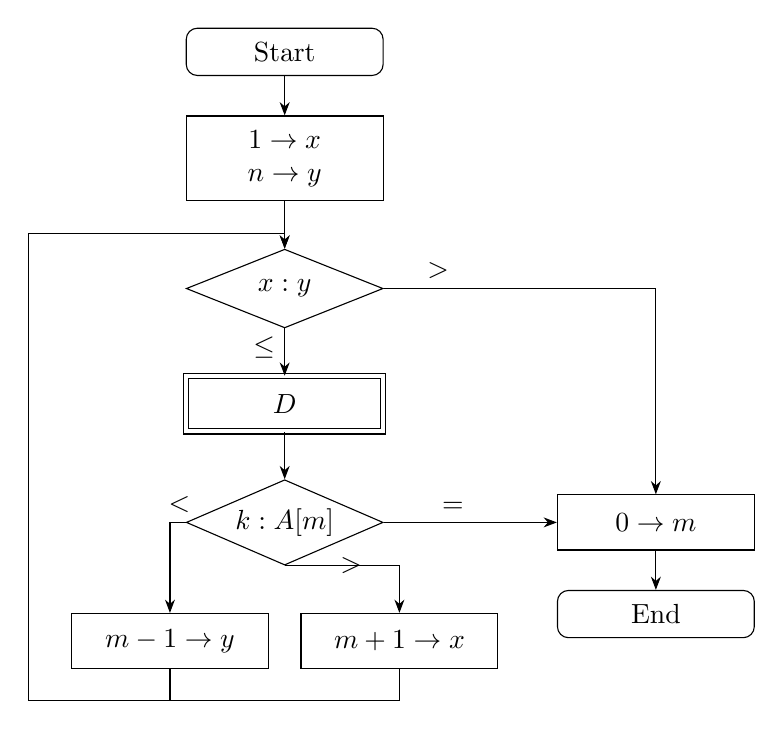
\begin{tikzpicture}[
        % Define block styles
        terminal/.style={draw, rectangle, rounded corners=4pt, minimum width=2.5cm, minimum height=0.6cm, text centered},
        process/.style={draw, rectangle, minimum width=2.5cm, minimum height=0.7cm, text centered},
        processD/.style={draw, double, double distance=1.5pt, rectangle, minimum width=2.5cm, minimum height=0.7cm, text centered},
        decision/.style={draw, diamond, aspect=2, minimum width=2.5cm, minimum height=1cm, text centered, inner sep=1pt},
        arrow/.style={draw, ->, >=Stealth}
    ]

    % --- Nodes Placement ---
    \node[terminal] (start) {Start};
    
    \node[process, below=0.5cm of start] (init) {
        \begin{tabular}{c}
        $1 \rightarrow x$ \\
        $n \rightarrow y$
        \end{tabular}
    };
    
    % Anchor node just above decision1 for loop line return alignment
    \node[circle, inner sep=0pt, minimum size=0pt, below=0.4cm of init] (loop_target) {};
    
    \node[decision, below=0.6cm of init] (dec1) {$x : y$};
    
    \node[processD, below=0.6cm of dec1] (boxD) {$D$};
    
    \node[decision, below=0.6cm of boxD] (dec2) {$k : A[m]$};
    
    % Branches below dec2
    \node[process, below left=0.6cm and 0.2cm of dec2.south] (branch_left) {$m-1 \rightarrow y$};
    \node[process, below right=0.6cm and 0.2cm of dec2.south] (branch_right) {$m+1 \rightarrow x$};
    
    % Right side termination path
    \node[process, right=2.2cm of dec2] (set_m) {$0 \rightarrow m$};
    \node[terminal, below=0.5cm of set_m] (end) {End};

    % --- Connections / Arrows ---
    \draw[arrow] (start) -- (init);
    \draw[arrow] (init) -- (dec1);
    \draw[arrow] (dec1) -- node[left, pos=0.4] {$\le$} (boxD);
    \draw[arrow] (boxD) -- (dec2);
    
    % Arrow from dec1 to set_m (greater-than branch)
    \draw[arrow] (dec1.east) -- node[above, pos=0.2] {$>$} (dec1.east -| set_m.north) -- (set_m.north);
    
    % Branches from dec2
    \draw[arrow] (dec2.west) -- node[above, pos=0.4] {$<$} (dec2.west -| branch_left.north) -- (branch_left.north);
    \draw[arrow] (dec2.south) -- node[right, pos=0.4] {$>$} (dec2.south -| branch_right.north) -- (branch_right.north);
    \draw[arrow] (dec2.east) -- node[above, pos=0.4] {$=$} (set_m.west);
    
    \draw[arrow] (set_m) -- (end);

    % Loop feedback paths back to the top
    % Left branch loop back
    \draw[arrow] (branch_left.south) -- ++(0,-0.4cm) -- ++(-1.8cm,0) |- (loop_target.center) -- (dec1.north);
    % Right branch loop back
    \draw[-] (branch_right.south) -- ++(0,-0.4cm) -- ++(-3.7cm,0); 

    \end{tikzpicture}
\end{center}

\noindent
Write an iterative C function for implementing the flowchart stated in the figure.

\mk{10} \yr{CSE 105 | L-1/T-2 | 2011--12}

%% Q24 — 2012-13
\item An Armstrong number of three digits is an integer such that the sum of the cubes of its digits equals the number itself (e.g., $153 = 1^3 + 5^3 + 3^3$). Write a C program to print all Armstrong numbers between 100 and 999.
\mk{10} \yr{CSE 105 | L-1/T-2 | 2010--11}

%% Q21 — 2010-11
\item Write a program to find whether $N$ is a super-prime or not. A number is super-prime if it and all its left-truncations are prime (e.g., 7331 is super-prime because 7331, 733, 73, and 7 are all prime; 4550 is not).
\mk{15} \yr{CSE 105 | L-1/T-2 | 2010--11}

%% Q22 — 2011-12
\item Write a program that can evaluate a mathematical expression of any length entered by a user, with \texttt{+}, \texttt{-}, \texttt{*}, and \texttt{/} operators and \texttt{double}-type operands in infix notation. For example: \texttt{4.0*6.5+32.0/4.0-10.45+5.5*7.25}.
\mk{10} \yr{CSE 101 | L-1/T-2 | 2009--10}

%% Q19 — 2009-10
\item Write a C program that will generate a table of values for the equation
\[ y = 2e^{-0.1t} \sin(0.5t) \]
where $t$ varies from 0 to 60. Allow the size of the $t$-increment to be entered as an input parameter. Use a macro to evaluate the formula.
\mk{10} \yr{CSE 101 | L-1/T-2 | 2009--10}

%% Q20 — 2010-11
\item Write a C program that determines the value of $x$ which causes the function $y = x\cos(x)$ to be maximized within a specified interval.
\mk{8} \yr{CSE 101 | L-1/T-2 | 2008--09}

%% Q18 — 2009-10
\item Write a simple program that will produce the following multiplication table using a loop.

\begin{center}
  \begin{tabular}{|>{\centering\arraybackslash}m{2.5em}|>{\centering\arraybackslash}m{2.5em}|>{\centering\arraybackslash}m{2.5em}|>{\centering\arraybackslash}m{2.5em}|>{\centering\arraybackslash}m{2.5em}|>{\centering\arraybackslash}m{2.5em}|}
        \hline
        1 & 2  & 3  & 4  & 5  & 6  \\ \hline
        2 & 4  & 6  & 8  & 10 & 12 \\ \hline
        3 & 6  & 9  & 12 & 15 & 18 \\ \hline
        4 & 8  & 12 & 16 & 20 & 24 \\ \hline
        5 & 10 & 15 & 20 & 25 & 30 \\ \hline
        6 & 12 & 18 & 24 & 30 & 36 \\ \hline
    \end{tabular}
\end{center}
\mk{10} \yr{CSE 105 | L-1/T-2 | 2005--06}

%% Q17 — 2008-09
\item Write a program that takes an integer $n$ as input. If the number is even, divide it by 2; otherwise multiply it by 3 and add 1. Continue until $n = 1$. Output the number of times the operations were executed. (For example, if $n = 3$ the answer is 7.)
\mk{7} \yr{CSE 101N | L-1/T-1 | 2003--04}

%% Q13 — 2003-04
\item For the following code sample, what is the final value of \texttt{i}?
 
\begin{lstlisting}
i = 0;
do {
    i = i + 1;
    if (i < 10) continue;
    i = i - 1;
} while (++i < 6);
\end{lstlisting}
\mk{4} \yr{CSE 101N | L-1/T-1 | 2003--04}

%% Q14 — 2003-04
\item When using the \texttt{continue} statement, the \texttt{for} loop behaves slightly differently from the corresponding \texttt{while} or \texttt{do-while} loop. Explain how.
\mk{4} \yr{CSE 101N | L-1/T-1 | 2003--04}

%% Q15 — 2003-04
\item Evaluate the cosine series:
\[
\cos(x) = 1 - \frac{x^2}{2!} + \frac{x^4}{4!} - \frac{x^6}{6!} + \cdots
\]
Assume $x$ ($0 < x < \pi$) is given in radians. Compute the value to some arbitrary precision using a loop.
\mk{6} \yr{CSE 101N | L-1/T-1 | 2003--04}

%% Q16 — 2005-06
\end{enumerate}

%%──────────────────────────────────────────────────────────────────────
\subtopic{cA}{Nested Control, break \& continue}
\label{sub:s2-nested}

\begin{enumerate}


%% Q7 — 2023-24
\item Assuming $N = 6$, analyse the following nested loop and find the corresponding output:
 
\begin{lstlisting}
for (i = 1; i <= N + 1; i++) {
    for (j = 1; j <= N; j++) {
        printf("%c", 'A' + ((i + j - 2) % N));
    }
    printf("\n");
}
\end{lstlisting}
\mk{10} \yr{CSE 101 | L-1/T-1 | 2023--24}

%% Q8 — 2010-11
\item What is the output of the following code? Assume \texttt{i} and \texttt{n} are integers.
 
\begin{lstlisting}
for (n = 1; n <= 5; n++)
    for (i = 1; i < n; i++)
        printf("%d%c", i, (i == n-1) ? '\n' : ',');
\end{lstlisting}
\mk{5} \yr{CSE 101 | L-1/T-1 | 2018--19}

\item Using nested loops, print an $N \times N$ grid where: (i) odd rows have $N$ plus signs and even rows have $N$ minus signs; (ii) odd columns have $N$ plus signs and even columns have $N$ minus signs. $N$ is input. (Show only the loop nesting, not the entire program.)
\begin{center}
  \begin{center}
\begin{tabular}{|l|l|}
\hline
\textbf{Example for 2(i): (suppose N=5)} & \textbf{Example 2(ii): (suppose N=5)} \\
\hline
\texttt{+ + + + +} & \texttt{+ - - - +} \\
\texttt{+ + + + +} & \texttt{- + - + -} \\
\texttt{+ + + + +} & \texttt{- - + - -} \\
\texttt{+ + - - -} & \texttt{- + - + -} \\
\texttt{+ + + + +} & \texttt{+ - - - +} \\
\hline
\end{tabular}
\end{center}
\end{center}
\mk{10} \yr{CSE 101 | L-1/T-1 | 2015--16}

%% Q10 — 2015-16 [Backlog]
\item Write a program that takes a positive integer $n$ as input and displays a pyramid pattern.
\begin{center}
\begin{lstlisting}
//For n=5,
        +
      + ^ +
    + ^ ^ ^ +
  + ^ ^ ^ ^ ^ +
+ + + + + + + + +
\end{lstlisting}
\end{center}
\mk{12} \yr{CSE 101 | L-1/T-1 | 2015--16}

%% Q11 — 2018-19
\item Rewrite the following code using \texttt{do-while} loops only:
 
\begin{lstlisting}
for (i = 1; i <= 5; i++) {
    for (j = 1; j <= i; j++)
        printf("%i", i);
    printf("\n");
}
\end{lstlisting}
\mk{5} \yr{CSE 105 | L-1/T-2 | 2010--11}

%% Q9 — 2015-16
\end{enumerate}

%%──────────────────────────────────────────────────────────────────────
\subtopic{cA}{\texttt{goto} Statement}
\label{sub:s2-goto}

\begin{enumerate}
%% Q16 — 2011-12
\item Why is it not encouraged to use the \texttt{goto} statement? Rewrite the following code segment without using \texttt{goto}:
 
\begin{lstlisting}
int a, b, c;
scanf("%d %d", &a, &b);
if (a < 0) goto label1;
if (b > 0) goto label2;
c = a;
goto label1;
label2: c = b;
label1:
\end{lstlisting}
\mk{10} \yr{CSE 105 | L-1/T-2 | 2007--08}


%% Q1 — 2003-04
\item Why is the use of the \texttt{goto} statement discouraged in structured programming? State a case in which \texttt{goto} is more useful than other control statements.
\mk{5} \yr{CSE 101N | L-1/T-1 | 2003--04}

\end{enumerate}
%% ══════════════════════════════════════════════════════════════════════
\secdivider{Part II}{Functions \& Arrays}{cB}{cB}

%% ── S3: Functions ─────────────────────────────────────────────────────
\section{S3 --- Functions}
\label{sec:S3}
\markboth{S3 --- Functions}{}

%%──────────────────────────────────────────────────────────────────────
\subtopic{cB}{Function Basics \& Parameter Passing}
\label{sub:s3-funcbasics}

\begin{enumerate}

%% Q9 — 2023-24
\item What is a function prototype? Explain with an example. Why do we need it?
\mk{5} \yr{CSE 101 | L-1/T-1 | 2024--25, 2023--24}

%% Q10 — 2022-23
\item Write down the output of the following program:
 
\begin{lstlisting}
#include <stdio.h>

void swap(int a, int b) {
    int *addressA = &a;
    int *addressB = &b;
    int *temp;
    temp = addressA;
    addressA = addressB;
    addressB = temp;
}

int main() {
    int a = 10;
    int b = 30;
    swap(a, b);
    printf("A=%d, B=%d", a, b);
    return 0;
}
\end{lstlisting}
\mk{7} \yr{CSE 101 | L-1/T-1 | 2022--23}

%% Q11 — 2022-23
\item What is the difference between pass by value and pass by reference?
\mk{5} \yr{CSE 101 | L-1/T-1 | 2022--23}

%% Q12 — 2003-04
\item Write down the output produced by the \texttt{printf} statements of the following \texttt{main} function:
 
\begin{lstlisting}
void swap(int x, int y, int *count) {
    static int i = 0;
    int t = x; x = y; y = t;
    i++;
    *count = i;
}
int main() {
    int a = 4, b = 5, count;
    swap(a, b, &count);
    printf("Swapping count %i %i %i", a, b, count);
    count = 3;
    swap(a, b, &count);
    printf("Swapping count %i %i %i", a, b, count);
}
\end{lstlisting}
\mk{3} \yr{CSE 101 | L-1/T-1 | 2021--22}

\item Write the following two functions for a degree-$n$ polynomial $p(x) = a_0 + a_1 x + \cdots + a_n x^n$:
\begin{enumerate}
  \item \texttt{double eval(double a[], double x, int n)} --- returns $p(x)$ evaluated at \texttt{x}.
  \item \texttt{void add(double f[], double g[], double h[], int n)} --- stores the sum of polynomials \texttt{g} and \texttt{h} (both of degree $\le n$) in \texttt{f}.
\end{enumerate}
\mk{12} \yr{CSE 101 | L-1/T-1 | 2018--19}

%% Q29 — 2021-22
\item Write a utility function \texttt{kSmooth(x, k)} that returns 1 if \texttt{x} is $k$-smooth (has no prime factors greater than $k$), and 0 otherwise.
\begin{center}
\begin{tabular}{|c|l|}
\hline
$k$ & $k$-smooth numbers \\
\hline
2 & 1, 2, 4, 8, 16, 32, 64, 128, 256, 512, \ldots \\
3 & 1, 2, 3, 4, 6, 8, 9, 12, 16, 18, 24, \ldots \\
4 & 1, 2, 3, 4, 5, 6, 8, 9, 10, 12, 15, 16, \ldots \\
5 & 1, 2, 3, 4, 5, 6, 8, 9, 10, 12, 15, 16, \ldots \\
\hline
\end{tabular}
\end{center}
\mk{13} \yr{CSE 101 | L-1/T-1 | 2015--16}

%% Q27 — 2015-16 [Backlog]
\item Write a function \texttt{int isPowerOfFive(int n)} that returns 1 if $n$ is a power of 5 and 0 otherwise. You are not allowed to use any library functions.
\begin{center}
\begin{tabular}{|l|c|}
\hline
\textbf{Function call} & \textbf{Return value} \\
\hline
\texttt{isPowerOfFive(5)}  & 1 \\
\texttt{isPowerOfFive(10)} & 0 \\
\texttt{isPowerOfFive(25)} & 1 \\
\texttt{isPowerOfFive(33)} & 0 \\
\hline
\end{tabular}
\end{center}
\mk{11} \yr{CSE 101 | L-1/T-1 | 2015--16}

%% Q28 — 2018-19
\item Write a function \texttt{double horner(double a[], int n, double x)} that uses Horner's rule to evaluate the polynomial $p(x) = a_0 + a_1 x + a_2 x^2 + \cdots + a_n x^n$. The array \texttt{a} has $n+1$ elements ($a_0$ to $a_n$); rewrite the evaluation as $a_0 + x(a_1 + x(a_2 + \cdots x(a_{n-1} + x \cdot a_n)\cdots))$.
\mk{12} \yr{CSE 105 | L-1/T-2 | 2014--15}

%% Q25 — 2014-15
\item Write a function \texttt{int checkFibonacci(int n)} that returns 1 if \texttt{n} is a Fibonacci number and 0 otherwise. (\texttt{checkFibonacci(8)} $\to$ 1; \texttt{checkFibonacci(21)} $\to$ 1; \texttt{checkFibonacci(7)} $\to$ 0.)
\mk{10} \yr{CSE 105 | L-1/T-2 | 2014--15}

%% Q26 — 2015-16
\item Given two integers $n$ and $x$ as parameters where $n > x > 1$, write a C function \texttt{int powerOfX(int n, int x)} that returns $y$ if $n = x^y$ for some $y \ge 0$, and $-1$ otherwise. For example, \texttt{powerOfX(125, 5)} returns 3 since $125 = 5^3$.
\mk{10} \yr{CSE 105 | L-1/T-2 | 2013--14}

%% Q22 — 2013-14
\item A Fermat number has the form $F_t = 2^{(2^t)} + 1$ (e.g., 3, 5, 17, 257, \ldots). Write a program that takes an integer $y$ as input and determines whether $y$ is a Fermat number, using the \texttt{powerOfX(n, x)} function from the previous question.
\mk{10} \yr{CSE 105 | L-1/T-2 | 2013--14}

%% Q23 — 2013-14
\item Write a program to calculate $\sqrt{x}$ where $x$ is a positive \texttt{double} value. You cannot use any library function.
\mk{10} \yr{CSE 105 | L-1/T-2 | 2013--14}


%% Q20 — 2012-13
\item Write down a C program to calculate $\sqrt{\lvert x \rvert}$ where $x$ is a \texttt{double} value. You cannot use any library function.
\mk{10} \yr{CSE 105 | L-1/T-2 | 2012--13}

%% Q21 — 2013-14
\item Describe the output of the following program:
 
\begin{lstlisting}
#include <stdio.h>
int a = 0, b = 1;
int funct1(int a);
int funct2(int b);
main() {
    int count;
    for (count = 1; count <= 5; ++count) {
        b += funct1(a + 1) + 1;
        printf("%d ", b);
    }
}
funct1(int a) {
    b = funct2(a + 1) + 1;
    return (b);
}
funct2(int a) {
    return (b + a);
}
\end{lstlisting}
\mk{15} \yr{CSE 105 | L-1/T-2 | 2011--12}

%% Q18 — 2011-12
\item What is a function prototype? Explain with an example. Write a C function named \texttt{swap} which inter-exchanges the values of \texttt{x} and \texttt{y} without declaring any variable within its body.
\mk{12} \yr{CSE 105 | L-1/T-2 | 2011--12}

%% Q19 — 2012-13
\item Describe the output of the following program:
 
\begin{lstlisting}
#include <stdio.h>
int a = 0, b = 1;
int funct1(int a);
int funct2(int b);
main() {
    for (int count = 1; count <= 5; ++count) {
        b += funct1(a + 1) + 1;
        printf("%d ", b);
    }
}
int funct1(int a) {
    static int c = 0;
    b = funct2(a + c++) + 1;
    return (b);
}
int funct2(int a) {
    if (a == 1) return (b + a);
    return (b + funct2(a - 1));
}
\end{lstlisting}
\mk{15} \yr{CSE 101 | L-1/T-2 | 2008--09}

%% Q17 — 2011-12
\item Write a function that can be used to sort any data type using the Quick Sort algorithm. Write also any necessary helper functions. Specify a comparison function for sorting structured data containing \texttt{name} (string) and \texttt{age} (\texttt{int}): sort in descending order of age; break ties by ascending order of name.
\mk{20} \yr{CSE 105 | L-1/T-2 | 2007--08}

%% Q16 — 2008-09
\item What is the difference between ``call by value'' and ``call by reference''? Explain with an example.
\mk{8} \yr{CSE 105 | L-1/T-2 | 2005--06}

%% Q14 — 2005-06
\item What does the \texttt{return} statement in the \texttt{main()} function indicate?
\mk{5} \yr{CSE 105 | L-1/T-2 | 2005--06}

%% Q15 — 2007-08
\item \textit{``In C, a call by reference is in fact one kind of call by value''} --- explain this statement.
\mk{5} \yr{CSE 101N | L-1/T-1 | 2003--04}

%% Q13 — 2005-06
\end{enumerate}

%%──────────────────────────────────────────────────────────────────────
\subtopic{cB}{Recursion}
\label{sub:s3-recursion}

\begin{enumerate}

%% Q10 — 2023-24
\item Write a recursive function \texttt{int strRlen(char s[])} that recursively determines and returns the length of a string. For example, \texttt{strRlen("DON'T UNDERESTIMATE THE POWER OF A COMMON MAN")} should return 45.
\mk{10} \yr{CSE 101 | L-1/T-1 | 2023--24}

%% Q11 — 2022-23
\item Write a recursive function in C to calculate the sum of the even digits of a positive integer. For example: input 123 $\to$ output 2; input 456 $\to$ output 10; input 135 $\to$ output 0.
\mk{15} \yr{CSE 101 | L-1/T-1 | 2022--23}

%% Q12 — 2003-04
\item Consider the following recursive function. Draw the recursive tree for the call \texttt{fib(6)} and write the output of the program:
 
\begin{lstlisting}
long fib(int num) {
    if (num <= 3) return 1;
    long val1 = fib(num-1);
    printf("%ld ", val1);
    long val2 = fib(num-2); 
    printf("%ld ", val2);
    long val3 = fib(num-3); 
    printf("%ld ", val3);
    return val1 + val2 + val3;
}
int main() {
   long ret = fib(6); 
   printf("\n%ld", ret); 
}
\end{lstlisting}
\mk{10} \yr{CSE 101 | L-1/T-1 | 2021--22}



%% Q35 — 2021-22
\item Write a recursive function \texttt{int rstrcmp(char s[], char t[], int i)} that compares two strings and returns 0 if equal, $-1$ if \texttt{s} lexicographically precedes \texttt{t}, and 1 otherwise. An initial call \texttt{rstrcmp(s, t, 0)} starts comparison from the beginning.
\mk{15} \yr{CSE 101 | L-1/T-1 | 2019--20}

%% Q34 — 2020-21
\item Write a recursive function \texttt{int largest(int x[], int n)} that returns the largest element in an array of \texttt{n} integers. Do not use loops, static, or global variables. Also write a simple \texttt{main} function demonstrating the initial call.
\mk{15} \yr{CSE 101 | L-1/T-1 | 2018--19}

%% Q32 — 2018-19
\item Write a recursive function \texttt{void printBinary(unsigned int x)} that prints the binary representation of \texttt{x} without leading zeros (except for 0 itself). Do not use loops, static, or global variables. No pre-processing in \texttt{main()}.
\mk{15} \yr{CSE 101 | L-1/T-1 | 2018--19}

%% Q33 — 2019-20
\item Consider the following \texttt{enigma} function:
 
\begin{lstlisting}
int enigma(int n) {
    if (n == 1) return 0;
    else return 1 + enigma(n / 2);
}
\end{lstlisting}
What will be the output if \texttt{enigma(4096)} is called from \texttt{main}? In one sentence, state what the function does. Assume $n > 0$.
\mk{7} \yr{CSE 101 | L-1/T-1 | 2015--16}

%% Q29 — 2015-16
\item Write a C function \texttt{decToBin(int num)} that returns the binary equivalent of a given integer using recursion.
\mk{8} \yr{CSE 101 | L-1/T-1 | 2015--16}

%% Q30 — 2015-16 [Backlog]
\item Write a recursive C function for binary search within a sorted list that returns the index of the element if found, or $-1$ otherwise.
\begin{lstlisting}
  int  binSearch(int* list, int low , int high, int value);
\end{lstlisting}
where list is the name of the sorted array and value is the element to be searched . Variables low and high represent the searching range.
\mk{10} \yr{CSE 101 | L-1/T-1 | 2015--16}

%% Q31 — 2018-19
\item Consider the following \texttt{enigma} function:
 
\begin{lstlisting}
void enigma(int n) {
    if (n != 0) enigma(n / 2);
    printf("%d", n % 2);
}
\end{lstlisting}
What will be the output if \texttt{enigma(13)} is called from \texttt{main}? In one sentence, state what the function does.
\mk{7} \yr{CSE 105 | L-1/T-2 | 2014--15}

%% Q26 — 2014-15
\item Calculate the value of $f(4)$ for the following recursive function:
\[ f(0) = 1, \qquad f(n) = n \times f(n-1) + n \]
\mk{6} \yr{CSE 105 | L-1/T-2 | 2014--15}

%% Q27 — 2014-15
\item Write a recursive C function \texttt{int count(char s[], char c)} that returns the number of occurrences of character \texttt{c} in string \texttt{s}. For example, \texttt{count("Toronto", 't')} $\to$ 1; \texttt{count("Toronto", 'o')} $\to$ 3. You must use recursion; no loops.
\mk{12} \yr{CSE 105 | L-1/T-2 | 2014--15}

%% Q25 — 2014-15
\item The Towers of Hanoi is played with three poles and $n$ disks of different sizes, initially stacked on the leftmost pole in decreasing size. The object is to transfer all disks to the rightmost pole, moving only one disk at a time and never placing a larger disk on a smaller one. Write a recursive C function that solves this problem and describe the output for $n = 4$. Also calculate the number of moves required to move $n$ disks.
\mk{15} \yr{CSE 105 | L-1/T-2 | 2012--13}

%% Q24 — 2013-14
\item A table contains $n$ unique data elements sorted in ascending order. The search algorithm splits the table into blocks of $m$ elements and performs a linear search on the last element of each block to find the target block. If the selected block has fewer than $m$ elements, a linear search is done on that block; otherwise the block is split into sub-blocks of $m$ and the process repeats recursively. Write a recursive C function implementing this searching algorithm for a list of integers.
\mk{10} \yr{CSE 105 | L-1/T-2 | 2011--12}

%% Q22 — 2011-12
\item Write a recursive C function to solve the Legendre Polynomials:
\[ P_n = \frac{2n-1}{n}\,x\,P_{n-1} - \frac{n-1}{n}\,P_{n-2} \]
where $P_0 = 1$, $P_1 = x$, and $x$ is any floating-point number in $[-1, 1]$. Describe the output of the function for $n = 5$ and $x = 0.5$.
\mk{13} \yr{CSE 105 | L-1/T-2 | 2011--12}

%% Q23 — 2012-13
\item The Legendre polynomials can be calculated by the formulas:
\[P_0 = 1,\quad P_1 = x,\quad P_n = \frac{2n-1}{n}\,x\,P_{n-1} - \frac{n-1}{n}\,P_{n-2}\quad (n=2,3,4,\ldots)\]
where $x$ is any floating-point number in $[-1,1]$. Write a C function \texttt{LP(n, x)} which returns the $n$-th Legendre polynomial value.
\mk{10} 
\\ Explain the output generated by the recursive function \texttt{LP(n, x)} described above for $n = 6$.
\mk{15} \yr{CSE 101 | L-1/T-2 | 2008--09}

%% Q21 — 2011-12
\item What is a recursive function? Describe its positive and negative aspects.
\mk{10} \yr{CSE 105 | L-1/T-2 | 2007--08}

%% Q17 — 2007-08
\item Let \texttt{array} be an external integer variable declared and initialized as follows. A \textit{cluster} of 1s in the array is defined recursively: search each position with value 1, and for each such position, search its eight neighbours for 1s, repeating recursively. Write a function that returns the number of clusters in the array. For example, the following array contains two clusters:
\begin{lstlisting}
int array[5][5] = {
    {1, 0, 0, 0, 1},
    {0, 1, 0, 1, 0},
    {0, 0, 1, 0, 0},
    {0, 1, 0, 1, 0},
    {1, 0, 0, 0, 1}
};
\end{lstlisting}
\mk{15} \yr{CSE 105 | L-1/T-2 | 2007--08}

%% Q18 — 2007-08
\item Write a recursive function prototyped as \texttt{void itob(char s[], int i)} which converts the integer \texttt{i} to its binary equivalent string in \texttt{s}.
\mk{10} \yr{CSE 105 | L-1/T-2 | 2007--08}


%% Q15 — 2005-06
\item Consider the following program code:
 
\begin{lstlisting}
int func(int a, int b) {
    if (b == 1) return a;
    else return a + func(a, b - 1);
}
\end{lstlisting}
\begin{enumerate}
  \item What does the above program do?
  \item What will be the output if \texttt{func(4, 4)} is called from \texttt{main()}?
  \item What will happen if \texttt{b} is less than 0?
  \item If the program does not give correct output for \texttt{b < 0}, fix the problem and rewrite the function.
\end{enumerate}
\mk{18} \yr{CSE 105 | L-1/T-2 | 2005--06}

%% Q19 — 2008-09
\item \textit{``Any problem that can be solved recursively can also be solved iteratively.''} Explain this statement with an example. Why and when will you prefer recursion to iteration?
\mk{12} \yr{CSE 105 | L-1/T-2 | 2005--06}

%% Q16 — 2007-08
\item You are given an already-built linked list of five nodes:
\begin{lstlisting}
struct node {
    int x;
    struct node *pnext;
};
\end{lstlisting}
The values in consecutive nodes starting at head \texttt{h} are 1, 2, 3, 4, and 5. Write a recursive function \texttt{void PrintList(struct node *ptr)} that prints the list in reverse order (i.e.\ outputs 5, 4, 3, 2, 1).
\mk{8} \yr{CSE 101N | L-1/T-1 | 2003--04}

%% Q13 — 2003-04
\item The sequence $T_n = \sum_{i=1}^{n} i$ generates the triangular numbers. The first four are 1, 3, 6, and 10. Write a recursive function \texttt{int Triangle(int n)} that takes a positive integer $n$ and returns $T_n$.
\mk{7} \yr{CSE 101N | L-1/T-1 | 2003--04}

\end{enumerate}

%% ── S4: Arrays & Strings ──────────────────────────────────────────────
\section{S4 --- Arrays \& Strings}
\label{sec:S4}
\markboth{S4 --- Arrays \& Strings}{}

%%──────────────────────────────────────────────────────────────────────
\subtopic{cB}{One-Dimensional Arrays: Searching \& Sorting}
\label{sub:s4-1darray}

\begin{enumerate}

    \item Write down a program that will take a set of integers as input in an array and will print only duplicate elements in the array. A duplicate element must be printed once. Also, you are not allowed to \textbf{change the content} of the array or use any \textbf{additional array}. The number of elements in the set, denoted by $N$, will also be input to your program.
    
    \vspace{0.3cm}
    \noindent \underline{\textbf{Sample Input/output}} \\
    N: 8 \\
    Enter array elements: 3 5 6 7 3 7 9 3 \\
    Duplicates: 3 7
    
    \vspace{0.6cm}
    \mk{17} \yr{CSE 101 | L-1/T-1 | 2024--25}

    
    \item Write a C program to input elements in a character array and find frequency of each character in the array. Assume that only capital letters will be input to your program. The number of characters will also be input to your program. Please also note the following couple of constraints:
    
    \begin{itemize}
        \item[(i)] Your program should have only one function called main() and no other functions.
        \item[(ii)] You \underline{cannot use any nested loop} to solve this problem but you can use more than one array if needed.
    \end{itemize}
    
    \vspace{0.3cm}
    \noindent \underline{\textbf{Sample Input/output}} \\
    Input size of array : 10 \\
    Input array elements: A B C A B D A Z X Z \\
    Output: \\
    Frequency of A = 3 \\
    Frequency of B = 2 \\
    Frequency of C = 1 \\
    Frequency of D = 1 \\
    Frequency of X = 1 \\
    Frequency of Z = 2
\mk{18} \yr{CSE 101 | L-1/T-1 | 2024--25}



%% Q10 — 2023-24
\item Write a C program that takes an array of integers as input and prints the following properties:
\begin{enumerate}
  \item \textbf{U/A/D} --- whether the array is Unsorted (\texttt{U}), sorted in Ascending (\texttt{A}) order, or Descending (\texttt{D}) order.
  \item \textbf{k} --- the largest difference between any two array elements.
  \item \textbf{f} --- the sum of the unique (non-duplicate) elements of the array.
\end{enumerate}
The output should be one character (\texttt{U}/\texttt{A}/\texttt{D}) followed by two integers ($k$ and $f$).
\mk{20} \yr{CSE 101 | L-1/T-1 | 2023--24}

%% Q11 — 2023-24
\item Research is a fascinating thing. The highest number of citations in a published
    research article doesn't really tell the full story about a researcher. In academia, we use a
    metric called h-index that measures both the productivity and citation impact of the
    publications of a researcher. It is defined as follows - the largest number $h$ such that $h$
    articles have at least $h$ citations each. For example, if an author has five publications,
    with, 9, 5, 4, 2, and 1 citations (ordered from greatest to least), then the author's h-index
    is 3, because the author has three publications with 3 or more citations. Write down a
    function \texttt{int calculateHindex(int C[], int N)} which takes an array $C$ containing the list of
    citations of the papers of an author, the size of the array $N$ and calculates the h-index of
    the author. Assume that the array elements will always be ordered from greatest to least.\mk{15} \yr{CSE 101 | L-1/T-1 | 2023--24}

%% Q12 — 2022-23
\item Write a C program that takes an integer $N$ as input, then reads $N$ numbers into an array, and prints the duplicate numbers (numbers that appear more than once).\\
\textit{Sample Input:} \texttt{5} / \texttt{1 2 2 3 1} \quad \textit{Sample Output:} \texttt{The duplicates are: 1 2}
\mk{12} \yr{CSE 101 | L-1/T-1 | 2022--23}

%% Q13 — 2022-23
\item Write a program that prints all elements present in array $A$ but \textbf{not} in array $B$ (set difference $A \setminus B$). The sizes and elements of both arrays are taken as input; all elements within each array are unique. For example, if $A = \{15, 7, 9\}$ and $B = \{1, 2, 3, 15\}$, the output is 7, 9.
\mk{13} \yr{CSE 101 | L-1/T-1 | 2022--23}

%% Q14 — 2003-04
\item Describe different ways to declare an integer array of size 100.
\mk{3} \yr{CSE 101 | L-1/T-1 | 2021--22}

%% Q33 — 2021-22
\item Write a function that takes four parameters: (i) an array, (ii) an element to insert, (iii) the index at which to insert it, and (iv) the current size of the array. The function inserts the element at the specified position.
\mk{8} \yr{CSE 101 | L-1/T-1 | 2021--22}

\item Write a C function \texttt{int deleteSorted(int x)} that deletes element \texttt{x} from a sorted integer array \texttt{A} of \texttt{N} elements (both declared globally). Returns the index from which the element was deleted, or $-1$ if not found. Assume no duplicate elements.
\mk{8} \yr{CSE 101 | L-1/T-1 | 2020--21}

%% Q31 — 2020-21
\item Write a complete C program to sort the following array of structs alphabetically by name. Break ties by placing the student with the lower ID first:
 
\begin{lstlisting}
struct student { int id; char name[50]; };
struct student students[50];
\end{lstlisting}
\mk{15} \yr{CSE 101 | L-1/T-1 | 2020--21}

%% Q32 — 2021-22
\item Write a program that prints all elements present in array \texttt{A} but not in array \texttt{B} (i.e., $A \setminus B$). Both arrays contain unique elements; their sizes and values are input. For example, $A=\{15,7,9\}$, $B=\{1,2,3,15\}$ $\to$ output 7, 9.
\mk{15} \yr{CSE 101 | L-1/T-1 | 2019--20}

%% Q30 — 2020-21
\item Write a function \texttt{void remove(int A[], int N, int V)} that searches if \texttt{V} exists in array \texttt{A} of \texttt{N} integers and removes the \textbf{last} occurrence of \texttt{V}, shifting each following element left and placing a zero at the end.
\mk{12} \yr{CSE 101 | L-1/T-1 | 2015--16}

%% Q28 — 2015-16 [Backlog]
\item Given two unsorted arrays \texttt{A} (size $m$) and \texttt{B} (size $n$), implement:
\begin{enumerate}
  \item \texttt{void union(int A[], int B[], int C[], int m, int n)} --- computes $C = A \cup B$.
  \item \texttt{void intersect(int A[], int B[], int D[], int m, int n)} --- computes $D = A \cap B$.
\end{enumerate}
\mk{18} \yr{CSE 101 | L-1/T-1 | 2015--16}

%% Q29 — 2019-20
\item Write a function \texttt{void remove(int A[], int N, int V)} that searches if \texttt{V} exists in array \texttt{A} of \texttt{N} integers and removes the first occurrence of \texttt{V}, shifting all subsequent elements left and placing a zero at the end.
\mk{12} \yr{CSE 105 | L-1/T-2 | 2014--15}

%% Q26 — 2014-15
\item Using the \texttt{qsort()} library function, you need to sort a list of strings lexicographically. Your input contains several lines. Each line contains a string (may contain spaces) of length no more than 32 characters. Process the input until the end of file is reached. The total number of strings will not exceed 150. After sorting, print out the strings according to the sort order. Recall that the \texttt{qsort()} library function has the following prototype:

\begin{lstlisting}
void qsort(
    void *Base,
    unsigned int NumOfElements,
    unsigned int SizeOf Eelments,
    int (*PtFuncCompare)(const void *, const void *)
);
\end{lstlisting}
\mk{10} \yr{CSE 105 | L-1/T-2 | 2014--15}

%% Q23 — 2013-14
\item Complete the definition of the C function \texttt{int maxCount(int list[], int length)} that returns the number of times the global maximum appears in the array. For example, in \texttt{\{3,9,7,5,9,8,2,4,9\}}, the global maximum is 9 and it appears 3 times, so the function returns 3.
\mk{12} \yr{CSE 105 | L-1/T-2 | 2013--14}

%% Q24 — 2013-14
\item Write a function \texttt{int nonrepeated(int a[], int n)} that returns the number of non-repeated elements in a sorted array \texttt{a} of length \texttt{n} (elements in ascending order, at least one element).
\mk{13} \yr{CSE 105 | L-1/T-2 | 2013--14}

%% Q25 — 2014-15
\item Write a C function \texttt{int countDistinct(int list[], int listLength)} where \texttt{list} is an integer array sorted in ascending (non-decreasing) order and \texttt{listLength} is its size. The function counts and returns the number of distinct elements. For example, \texttt{\{1,1,3,3,3,3,6,8,8,9,9,9,9,9\}} $\to$ 5.
\mk{15} \yr{CSE 105 | L-1/T-2 | 2012--13}

%% Q21 — 2013-14
\item Write a C function to delete an integer element from a sorted array.
\mk{10} \yr{CSE 105 | L-1/T-2 | 2011--12}

%% Q20 — 2012-13
\item Write a program to enter $n$ elements in an array and find the second smallest number from the array. There must be no nested loops in your program.
\mk{10} \yr{CSE 105 | L-1/T-2 | 2010--11}

%% Q19 — 2011-12
\item Write a print function to print the elements of a triangular array (see dynamic memory allocation questions) from the top to the bottom.
\mk{7} \yr{CSE 101 | L-1/T-2 | 2009--10}

%% Q17 — 2009-10
\item In merge sort, sorting a sequence $S$ with $n$ elements uses three divide-and-conquer steps: (i) if $S$ has zero or one element, return immediately; (ii) divide $S$ into two sequences $S_1$ and $S_2$ each of about $n/2$ elements; (iii) recursively sort $S_1$ and $S_2$, then merge them. Implement this merge sort algorithm for a one-dimensional array of $n$ elements.
\mk{10} \yr{CSE 101 | L-1/T-2 | 2009--10}

%% Q18 — 2010-11
\item Consider a 2-dimensional array of integers which are row-wise and column-wise unsorted. Write a C function that sorts the integers such that the array becomes row-wise sorted.
\mk{10} \yr{CSE 101 | L-1/T-2 | 2008--09}

%% Q16 — 2009-10
\item Write a function that takes an array of integers and its size as parameters and returns the element that appears the maximum number of times. For example, for \texttt{a[] = \{1,5,4,4,2,6,4\}} it returns 4 (appears 3 times). For multiple such elements, return the first one.
\mk{8} \yr{CSE 101N | L-1/T-1 | 2003--04}

%% Q15 — 2008-09
\end{enumerate}

%%──────────────────────────────────────────────────────────────────────
\subtopic{cB}{Character \& String Operations}
\label{sub:s4-strings}

\begin{enumerate}

\item "Array of characters and string are same" - Justify. Explain different ways to represent string with examples.
\mk{7} \yr{CSE 101 | L-1/T-1 | 2024--25}

    \item Take two strings as input. Next, from the first string, delete the characters that are in the second string. Output the remainder of the first string.
    \mk{8} \yr{CSE 101 | L-1/T-1 | 2024--25}

    \item You are to implement \textbf{\textit{strchrs}} function, which can search for more than one characters in a string and returns the location of the characters. In this case, all the search keyword characters are to be given within another string as parameter. Every time \textit{strchrs} is called, it returns the index of the string containing the location of one of the search characters in the string. At first the function will be called by the string as parameter and it will return the index of the first location. To get the subsequent location NULL is passed as parameter to \textit{strchrs}. If a new string is given instead of NULL, then finding subsequent locations takes place on the new string. If there is no other characters in the string it will return -1.
    \mk{12} \yr{CSE 101 | L-1/T-1 | 2024--25}

    \item Write functions to implement the following:
    \begin{itemize}
        \item[(i)] copying a string to another string
        \item[(ii)] Comparing two strings
    \end{itemize}  
\mk{$4\times2=8$} \yr{CSE 101 | L-1/T-1 | 2024--25}


%% Q10 — 2023-24
\item What is the necessity of the null character (\texttt{'\textbackslash 0'}) in defining a string in C? Explain with necessary examples.
\mk{6} \yr{CSE 101 | L-1/T-1 | 2023--24}

%% Q11 — 2023-24
\item Implement the \texttt{strtok} function that can search for more than one separator character in a string, where all separator characters are provided as a second string parameter. The first parameter is the string to be tokenised. Each call returns the address of the next token. On the first call, pass the source string; on subsequent calls, pass \texttt{NULL} to continue tokenising. If a new non-\texttt{NULL} string is passed, tokenisation restarts on that string.
\mk{12} \yr{CSE 101 | L-1/T-1 | 2023--24}

%% Q12 — 2023-24
\item You are given the hexadecimal string \texttt{"A7B8"}. First convert it to a decimal number, then convert that number to an octal string and output it. For \texttt{"A7B8"} the expected output is \texttt{"123670"}.
\mk{9} \yr{CSE 101 | L-1/T-1 | 2023--24}

%% Q14 — 2022-23
\item Write a C function that converts an input integer into its equivalent string representation. For example, input 523 should produce the string \texttt{"523"}. The scope of the returned string must be accessible from \texttt{main}.
\mk{15} \yr{CSE 101 | L-1/T-1 | 2022--23}

%% Q15 — 2022-23
\item Complete the following C code to reverse a string \textbf{without} using any library function from \texttt{<string.h>}. Write your code with proper comments for the missing part only.
 
\begin{lstlisting}
#include <stdio.h>
int main() {
    char str[100], reversedStr[100];
    gets(str);
    // add your code here
    // start of your code

    // end of your code
    puts(reversedStr);
    return 0;
}
\end{lstlisting}
\mk{12} \yr{CSE 101 | L-1/T-1 | 2022--23}

%% Q16 — 2022-23
\item Implement a Caesar Cipher in C: shift each character in the string forward by 2 positions (wrapping around). Assume all characters are lowercase letters. Examples: \texttt{"abc"} $\to$ \texttt{"cde"}, \texttt{"xyz"} $\to$ \texttt{"zab"}.
\mk{12} \yr{CSE 101 | L-1/T-1 | 2022--23}

%% Q17 — 2003-04
\item Define the string data type. How is a string data type implemented in C?
\mk{5} \yr{CSE 101 | L-1/T-1 | 2021--22}

%% Q47 — 2021-22
\item Take two strings as input. Check whether the first string occurs inside the second one, and if so, output how many times. For example, \texttt{"desh"} is in \texttt{"Bangladesh"} once; \texttt{"aa"} is in \texttt{"aaa"} twice.
\mk{8} \yr{CSE 101 | L-1/T-1 | 2021--22}

%% Q48 — 2021-22
\item Write a program that takes an integer in decimal format from the keyboard and converts it to a string of hexadecimal format. Do not use any built-in function.
\mk{10} \yr{CSE 101 | L-1/T-1 | 2021--22}

%% Q49 — 2021-22
\item Write the following string functions using pointer manipulation (no array indexing):
\begin{enumerate}
  \item \texttt{strcpy} --- copies one string to another.
  \item \texttt{strcmp} --- compares two strings.
  \item \texttt{strcat} --- concatenates two strings.
\end{enumerate}
\mk{12} \yr{CSE 101 | L-1/T-1 | 2021--22}

\item Write a C function \texttt{char *dbl\_dbl(char *str, char ch)} that returns a new string where every single occurrence of character \texttt{ch} in \texttt{str} is doubled. Double occurrences are left unchanged.\\
\textit{Examples:} \texttt{dbl\_dbl("baba", 'a')} $\to$ \texttt{"baabaa"}; \quad \texttt{dbl\_dbl("aa", 'a')} $\to$ \texttt{"aaaa"}.
\mk{15} \yr{CSE 101 | L-1/T-1 | 2020--21}

%% Q46 — 2021-22
\item Write a program that searches for the reverse of a given word within a sentence. Both word and sentence are input. If found, print the first position only; otherwise print \texttt{NOT FOUND}.
\mk{15} \yr{CSE 101 | L-1/T-1 | 2019--20}

%% Q44 — 2019-20
\item Write a function that counts the number of words in a string. Words are separated by one or more white-space characters.
\mk{15} \yr{CSE 101 | L-1/T-1 | 2019--20}

%% Q45 — 2020-21
\item Write a function to calculate and return the length of a string passed as a parameter. Do not use \texttt{<string.h>}.
\mk{5} \yr{CSE 101 | L-1/T-1 | 2018--19}

%% Q40 — 2018-19
\item Write a program to perform lexicographical comparison between two strings.
\mk{10} \yr{CSE 101 | L-1/T-1 | 2018--19}

%% Q41 — 2018-19
\item Write a program that takes a string (no spaces) followed by a character, separated by a single space. Delete all occurrences of the character from the string. Store the string in a \texttt{char} array called \texttt{str}; do not declare any other arrays. Do not use \texttt{<string.h>}.\\
\textit{Example:} \texttt{str = "abcbabxy"}, \texttt{c = 'b'} $\to$ \texttt{"acaxy"}.
\mk{10} \yr{CSE 101 | L-1/T-1 | 2018--19}

%% Q42 — 2018-19
\item Write a program that takes 2 strings (may contain spaces) as input and prints their longest common substring. If there are multiple longest common substrings, print any one. For example, for \texttt{"abcdef"} and \texttt{"ceddefg"}, the longest common substring is \texttt{"def"}.
\mk{15} \yr{CSE 101 | L-1/T-1 | 2018--19}

%% Q43 — 2019-20
\item Write C code to implement the following string functions using only pointer arithmetic (no array indexing):
\begin{enumerate}
  \item \texttt{char *strncat(char *dest, char *src, size\_t n)} --- appends up to $n$ characters from \texttt{src} to \texttt{dest}.
  \item \texttt{char *strchr(char *str, int c)} --- finds the first occurrence of character \texttt{c} in \texttt{str}.
  \item \texttt{int strcmp(char *str1, char *str2)} --- compares two strings.
  \item \texttt{int strlen(char *str)} --- returns the length of \texttt{str}.
  \item \texttt{char *strstr(char *haystack, char *needle)} --- finds the first occurrence of \texttt{needle} in \texttt{haystack}.
\end{enumerate}
\mk{18} \yr{CSE 101 | L-1/T-1 | 2015--16}

%% Q37 — 2015-16 [Backlog]
\item Write a program that takes an integer (positive or negative) as input and prints it in comma-separated format (a comma after every three digits from the right).
\begin{center}
\begin{tabular}{rr}
\hline
\textbf{Sample inputs} & \textbf{Sample outputs} \\
\hline
-1234567890 & -1,234,567,890 \\
-123456     & -123,456       \\
-12345      & -12,345        \\
-1000       & -1,000         \\
-999        & -999           \\
-1          & -1             \\
0           & 0              \\
1           & 1              \\
999         & 999            \\
1000        & 1,000          \\
12345       & 12,345         \\
123456      & 123,456        \\
1234567890  & 1,234,567,890  \\
\hline
\end{tabular}
\end{center}

\mk{15} \yr{CSE 101 | L-1/T-1 | 2015--16}

%% Q38 — 2015-16 [Backlog]
\item Write a C function that returns the index of the first occurrence of a substring in a string. Pass the string as the first argument and the substring as the second. Use pointers and avoid array indexing.
\begin{lstlisting}
  int findSubStrIndex(const char* str, const char* substr);
\end{lstlisting}
For example findSubStrIndex("This is a pen", "is") will return 2, while findSubStrIndex("This is a pen", "ball") will return -1 .
\mk{10} \yr{CSE 101 | L-1/T-1 | 2015--16}

%% Q39 — 2018-19
\item A substring of a string $S$ is another string $S'$ that occurs in $S$. For example, ``the best of'' is a substring of ``It was the best of times''. Given, 2 strings $s$ and $t$, you need to detect whether $t$ is a substring of $s$. Solve this problem by implementing the function declared below. You don't need to write \texttt{main()} or any \texttt{scanf}/\texttt{printf} statements. Note: You cannot use \texttt{string.h} header for this task.

\begin{lstlisting}
// return 1 if t is a substring of s
// return 0 otherwise
int isSubstring(char *s, char *t);
\end{lstlisting}
\mk{15} \yr{CSE 105 | L-1/T-2 | 2014--15}

%% Q35 — 2014-15
\item The \textit{longest common substring} problem is to find the longest sting that is a substring of two strings. For example, the longest common substring of the strings ``ABABC'', and ``BABCAB'' is string ``BABC'' of length 4. Other common substrings are ``A'', ``AB'', ``B'', ``BA'', ``BAB'', ``ABC'', ``BC'' and ``C''. Given 2 strings $s$ and $t$, you need to find the length of their longest common substring. Solve this problem by implementing the function declared below. You don't need to write \texttt{main()} or any \texttt{scanf}/\texttt{printf} statements. \\
\underline{Note: You cannot use \texttt{string.h} header for this task. You can use the functions you} \underline{implemented in answering the previous question .}

\begin{lstlisting}
//
//return the length of longest common substring of s and t
//
int longestCommonSubstringLength(char *s, char *t);
\end{lstlisting}
\mk{10} \yr{CSE 105 | L-1/T-2 | 2014--15}

%% Q36 — 2015-16
\item Write a C function \texttt{int strpos(const char *str, char ch)} that finds the first occurrence of character \texttt{ch} in string \texttt{str} and returns its 0-based position index, or $-1$ if not found.
\mk{10} \yr{CSE 105 | L-1/T-2 | 2012--13}

%% Q34 — 2014-15
\item A C program contains the array declaration \texttt{char text[100];}. The string \texttt{"Programming with C can be a challenging creative activity."} is assigned to \texttt{text}. Show the output of the following \texttt{printf()} statements (use \texttt{|\_|} to represent each blank):
\begin{enumerate}
  \item \texttt{printf("\%18s", text);}
  \item \texttt{printf("\%.18s", text);}
  \item \texttt{printf("\%18.7s", text);}
  \item \texttt{printf("\%-18.7s", text);}
\end{enumerate}
 
\mk{8} \yr{CSE 105 | L-1/T-2 | 2011--12}

%% Q33 — 2012-13
\item Write a function \texttt{char *reverseword(char *s)} which takes a string as input, detects each word, reverses each word (leaving blanks intact), and returns a pointer to the resultant string.
\mk{15} \yr{CSE 105 | L-1/T-2 | 2010--11}

%% Q31 — 2010-11
\item Write a function \texttt{int strrindex(char s[], char t[])} that returns the position of the rightmost occurrence of string \texttt{t} in string \texttt{s}, or $-1$ if there is no such occurrence.\\
\textit{Sample:} \texttt{s="aabcaabc"}, \texttt{t="aa"} $\to$ 4; \quad \texttt{s="aabcacacd"}, \texttt{t="bc"} $\to$ 2; \quad \texttt{s="abcabcabc"}, \texttt{t="abcd"} $\to$ $-1$.
\mk{12} \yr{CSE 105 | L-1/T-2 | 2010--11}

%% Q32 — 2011-12
\item Implement \texttt{char *strtok(char *str, char *ptrn)} with its usual functionality as defined in \texttt{<string.h>} using a local static string variable.
\mk{17} \yr{CSE 101 | L-1/T-2 | 2009--10}

%% Q29 — 2009-10
\item Write a function \texttt{char *strdel(char *s1, char *s2, int n)} that deletes each character from the string \texttt{s1} that matches any character in \texttt{s2} \textbf{and} appears more than $n$ times in \texttt{s1}. The function should return the resultant string while leaving \texttt{s1} unchanged.
\mk{17} \yr{CSE 101 | L-1/T-2 | 2009--10}

%% Q30 — 2010-11
\item Provide definitions for each of the following function declarations. Your code should use pointer arithmetic and avoid array indexing:
\begin{enumerate}
  \item \texttt{int strrspn(char *cs, char *ct);} --- return the length of the suffix (end) of \texttt{cs} consisting of characters in \texttt{ct}.
  \item \texttt{int strseq(char *cs, char *ct);} --- return 1 if \texttt{ct} is a subsequence of \texttt{cs}, otherwise return 0. (\texttt{ct} is a subsequence of \texttt{cs} if all characters of \texttt{ct} appear in \texttt{cs} in the same relative order.)
\end{enumerate}
\mk{12} \yr{CSE 101 | L-1/T-2 | 2008--09}

%% Q27 — 2008-09
\item What will be the output of the following code segment?
 
\begin{lstlisting}
char *p = "ctrl", *q = "alt", c, d;
c = *++p;
d = ++*q;
printf("%c %s\n%c %s", c, p, d, q);
\end{lstlisting}
\mk{10} \yr{CSE 101 | L-1/T-2 | 2008--09}

%% Q28 — 2009-10
\item Write each of the following functions:
\begin{enumerate}
  \item \texttt{int strncmp(char *cs, char *ct, int n)} --- compare at most $n$ characters of string \texttt{cs} to \texttt{ct}; return $<0$ if \texttt{cs}$<$\texttt{ct}, $0$ if equal, $>0$ if \texttt{cs}$>$\texttt{ct} up to $n$ characters.
  \item \texttt{int strspn(char *cs, char *ct)} --- return the length of the prefix of \texttt{cs} consisting entirely of characters in \texttt{ct}.
  \item \texttt{char *strrstr(char *cs, char *ct)} --- return a pointer to the last (rightmost) occurrence of string \texttt{ct} in \texttt{cs}, or \texttt{NULL} if not present.
\end{enumerate}
\mk{18} \yr{CSE 105 | L-1/T-2 | 2007--08}

%% Q23 — 2007-08
\item Write a function prototyped as \texttt{int strrindex(char s[], char t[])} which returns the position of the rightmost occurrence of \texttt{t} in \texttt{s}, or $-1$ if there is none.
\mk{10} \yr{CSE 105 | L-1/T-2 | 2007--08}

%% Q24 — 2007-08
\item Write a function prototyped as \texttt{void insert\_str\_at(char dest[], char src[], int pos)} which inserts the string \texttt{src} into the string \texttt{dest} starting at position \texttt{pos}.
\mk{10} \yr{CSE 105 | L-1/T-2 | 2007--08}

%% Q25 — 2007-08
\item Write a function \texttt{void str\_str(char src[], char substr[], int ith)} which copies the $i$-th whitespace-separated substring of \texttt{src} into \texttt{substr}. Whitespace delimiters are \texttt{'\textbackslash n'}, \texttt{'\textbackslash t'}, and \texttt{' '}. For example, if \texttt{src[] = "abc def efg hij"} and \texttt{ith = 2}, then \texttt{"def"} is copied to \texttt{substr}.
\mk{10} \yr{CSE 105 | L-1/T-2 | 2007--08}

%% Q26 — 2008-09
\item Write a C program that will take a sentence as input and print whether it is a palindrome or not. A palindrome is a sentence that reads the same forwards and backwards.
\mk{10} \yr{CSE 105 | L-1/T-2 | 2005--06}

%% Q21 — 2005-06
\item Implement the following string functions (write down the C code for each function, not a complete program):
\begin{enumerate}
  \item \texttt{int strlen(char *str);}
  \item \texttt{char *strcat(char *str1, char *str2);}
  \item \texttt{char *strcpy(char *str1, char *str2);}
  \item \texttt{char *strchr(char *str, char c);}
\end{enumerate}
\mk{20} \yr{CSE 105 | L-1/T-2 | 2005--06}

%% Q22 — 2007-08
\item Write a function \texttt{void Encrypt(char *s, int key)} that encrypts a string by shifting every letter forward by \texttt{key} positions (wrapping around from \texttt{'z'} back to \texttt{'a'}). For example, \texttt{"zany"} encrypted with key 4 yields \texttt{"derc"}.
\mk{10} \yr{CSE 101N | L-1/T-1 | 2003--04}

%% Q18 — 2003-04
\item Write a program that queries the user for two phrases and indicates whether they are anagrams (every letter appears the same number of times in each phrase). The comparison should be case-insensitive and ignore non-alphabet characters. Assume all inputs are at most 80 characters.\\
\textit{Sample:} \texttt{"Dirty room"} and \texttt{"Dormitory"} $\to$ anagrams.
\mk{12} \yr{CSE 101N | L-1/T-1 | 2003--04}

%% Q19 — 2003-04
\item Write a function \texttt{void KillSpaces(char *s)} that removes all space characters from a string in-place. The function prototype is given.
\mk{7} \yr{CSE 101N | L-1/T-1 | 2003--04}

%% Q20 — 2005-06
\end{enumerate}

%%──────────────────────────────────────────────────────────────────────
\subtopic{cB}{Multi-Dimensional Arrays \& Matrix Operations}
\label{sub:s4-2darray}

\begin{enumerate}

%% Q8 — 2023-24
\item Consider a three-dimensional array with dimensions $l \times m \times n$. An element is indicated by \texttt{A[i][j][k]}. What is the equivalent index of this element for a one-dimensional (flattened) array?
\mk{6} \yr{CSE 101 | L-1/T-1 | 2023--24}

%% Q9 — 2023-24
\item Define a two-dimensional array to store the marks of $m$ subjects for $n$ students (both $n$ and $m$ taken as input). After reading all marks, output:
\begin{enumerate}
  \item The total marks for each student.
  \item The highest mark for each subject.
\end{enumerate}
\mk{10} \yr{CSE 101 | L-1/T-1 | 2023--24}

%% Q10 — 2023-24
\item Write a program that demonstrates the addition, subtraction, and multiplication of two matrices. Requirements:
\begin{itemize}
  \item A function to input elements of a matrix.
  \item The program asks for matrix dimensions and allocates memory dynamically for exactly those dimensions.
  \item Addition, subtraction, and multiplication functions each create a new resultant matrix.
  \item A function to free the allocated memory for a matrix.
  \item A function to print a matrix in a formatted way.
  \item \textbf{You are not allowed to use array declaration or array indexing anywhere in this program.}
\end{itemize}
\mk{18} \yr{CSE 101 | L-1/T-1 | 2023--24}

%% Q11 — 2022-23
\item Write a function in C that takes a square matrix as input and prints:
\begin{enumerate}
  \item The maximum value among the diagonal elements.
  \item The minimum value among the non-diagonal elements.
\end{enumerate}
\mk{15} \yr{CSE 101 | L-1/T-1 | 2022--23}

%% Q12 — 2003-04
\item Write a program that demonstrates addition, subtraction, and multiplication of two matrices. Requirements:
\begin{itemize}
  \item A function to input matrix elements.
  \item Ask for dimensions and allocate memory dynamically for exactly those dimensions.
  \item Each operation function creates a new resultant matrix.
  \item A function to free the allocated memory.
  \item A function to print a matrix in a formatted way.
\end{itemize}
\mk{22} \yr{CSE 101 | L-1/T-1 | 2021--22}

\item Write a complete C program that takes two integer matrices (not necessarily square) as input, multiplies them, and displays the result. Read the sizes and elements from input; use prompt messages and proper indentation. Use the minimum number of variables.
\mk{10} \yr{CSE 101 | L-1/T-1 | 2020--21}

%% Q28 — 2021-22
\item Write a program that counts and prints the number of non-repeated elements located within the two diagonals of an $M \times N$ matrix \texttt{A}. For the matrix $\begin{pmatrix}1&2&1\\3&3&4\\5&6&7\end{pmatrix}$, the answer is 2 (only 5 and 7).
\mk{15} \yr{CSE 101 | L-1/T-1 | 2019--20}

%% Q26 — 2019-20
\item Write a function 
\begin{lstlisting}
  int** mult(int** A, int rA, int cA, int** B, int rB, int cB); 
 \end{lstlisting} 
that performs matrix multiplication. Dynamically allocate memory for the result and return a pointer to it; return \texttt{NULL} if multiplication is not possible. Also write \texttt{main} to read two matrices from the console using dynamic memory, call \texttt{mult}, and print the result.
\mk{20} \yr{CSE 101 | L-1/T-1 | 2019--20}

%% Q27 — 2020-21
\item Write code to fill an $N \times N$ matrix \texttt{A[N][N]} with the following pattern ($N$ is input): upper-left triangle filled with 1s, the anti-diagonal with 0s, and the lower-right triangle with $-1$s.

\begin{center}
\renewcommand{\arraystretch}{1.3} % Adds professional padding to match the image grid
\begin{tabular}{|c|c|c|c|c|c|}
\hline
1 &  1 &  1 &  1 &  1 &  0 \\ \hline
1 &  1 &  1 &  1 &  0 & -1 \\ \hline
1 &  1 &  1 &  0 & -1 & -1 \\ \hline
1 &  1 &  0 & -1 & -1 & -1 \\ \hline
1 &  0 & -1 & -1 & -1 & -1 \\ \hline
0 & -1 & -1 & -1 & -1 & -1 \\ \hline
\end{tabular}
\end{center}
\mk{10} \yr{CSE 101 | L-1/T-1 | 2018--19}

%% Q24 — 2018-19
\item Write a function \texttt{int ALTERSUM(int N, int M, int B[][M])} that finds and returns the sum of every alternate element of a 2-D array \texttt{B} (with $N$ rows and $M$ columns), starting from \texttt{B[0][0]}.
\mk{13} \yr{CSE 101 | L-1/T-1 | 2018--19}

%% Q25 — 2019-20
\item A magic square is a square matrix of distinct numbers (each number is used only
    once), where the numbers in each row, and the numbers in each column, and the numbers
    in each diagonal, all add up to the same number. For example, the following is a magic
    square where the numbers in each row, and in each column and, in each diagonal add up
    to 15.

    \begin{center}
    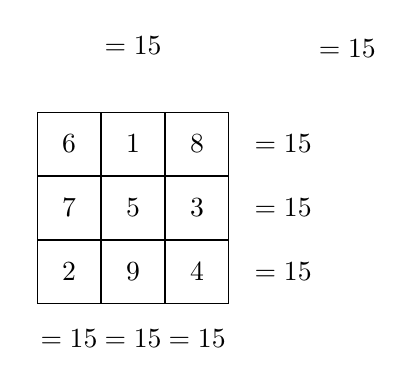
\begin{tikzpicture}
        \matrix (m) [matrix of nodes,
            nodes={draw, minimum size=8mm, anchor=center},
            column sep=0pt, row sep=0pt]
        {
            6 & 1 & 8 \\
            7 & 5 & 3 \\
            2 & 9 & 4 \\
        };
        % Row sums
        \node[draw=none] at (m-1-3.east) [right=2mm] {$= 15$};
        \node[draw=none] at (m-2-3.east) [right=2mm] {$= 15$};
        \node[draw=none] at (m-3-3.east) [right=2mm] {$= 15$};
        % Column sums
        \node[draw=none] at (m-3-1.south) [below=2mm] {$= 15$};
        \node[draw=none] at (m-3-2.south) [below=2mm] {$= 15$};
        \node[draw=none] at (m-3-3.south) [below=2mm] {$= 15$};
        % Top labels
        \node[draw=none] at (m-1-1.north) [above=2mm] {};
        \node[draw=none] at (m-1-2.north) [above=6mm] {$= 15$};
        % Diagonal label (top right)
        \node[draw=none] at ([xshift=15mm, yshift=8mm]m-1-3.north east) {$= 15$};
    \end{tikzpicture}
    \end{center}


Write a C function \texttt{isMagicSquare(int n, int A[][n])} that returns 1 if the $n \times n$ matrix \texttt{A} is a magic square
, and 0 otherwise.
\mk{13} \yr{CSE 101 | L-1/T-1 | 2015--16}

%% Q19 — 2015-16
\item Write a C function \texttt{getMinOfArray} with proper parameters that takes a three-dimensional array and returns its minimum element. You may add parameters but cannot declare global variables.
\mk{7} \yr{CSE 101 | L-1/T-1 | 2015--16}

%% Q20 — 2015-16 [Backlog]
\item Define three $100 \times 100$ integer arrays. Read the number of rows $m$ and columns $n$, then read $m \times n$ integers for the first two arrays. Perform matrix multiplication and store the result in the third array.
\mk{10} \yr{CSE 101 | L-1/T-1 | 2015--16}

%% Q21 — 2015-16 [Backlog]
\item Write a C function to calculate the transpose of a square matrix.
\begin{lstlisting}
  void transpose(int* list, int n);
  //list represents the matrix
  //n is the number of rows/columns
\end{lstlisting}

\mk{10} \yr{CSE 101 | L-1/T-1 | 2015--16}

%% Q22 — 2015-16 [Backlog]
\item A gray scale image is represented by a 2-dimensional integer array where value of each
    pixel represented by a number ranges from 0 to 255. A sample gray image is given
    below:

    \begin{center}
    \begin{tabular}{|c|c|c|c|c|c|}
    \hline
    231 & 187 & 178 & 194 & 203 & 190 \\
    \hline
    202 & 195 & 198 & 195 & 204 & 192 \\
    \hline
    214 & 197 & 179 & 196 & 200 & 197 \\
    \hline
    230 & 190 & 180 & 198 & 201 & 187 \\
    \hline
    224 & 219 & 193 & 200 & 201 & 186 \\
    \hline
    231 & 123 & 189 & 201 & 203 & 197 \\
    \hline
    \end{tabular}
    \end{center}

    An error matrix is calculated as follows. At first average of all the pixels are calculated
    and then error of each pixel is calculated by subtracting the average from the pixel value.
    Write a C function to calculate error matrix of a given image. Also write a C function to
    calculate the error frequency list, which represents how many times each error occurs.
    Arrange the list in ascending order on error values.
\mk{15} \yr{CSE 101 | L-1/T-1 | 2015--16}

%% Q23 — 2018-19
\item Implement a function \texttt{diagonalsSum} that returns the sum of the elements of both diagonals of an $n \times n$ matrix. Design the parameter list appropriately. Also write a \texttt{main} function to read $n$ ($1 \le n \le 10$) and the matrix, then call \texttt{diagonalsSum} and print the result. Do not use global variables.
\mk{15} \yr{CSE 105 | L-1/T-2 | 2014--15}

%% Q18 — 2015-16
\item Write a program to sort all elements in a $4 \times 4$ matrix row-wise.
\begin{center}
  \begin{equation*}
\text{Input: } 
\begin{bmatrix}
4 & 3 & 2 & 1 \\
4 & 3 & 3 & 1 \\
4 & 3 & 2 & 1 \\
4 & 3 & 2 & 2
\end{bmatrix}
\qquad\qquad \text{Output: }
\begin{bmatrix}
1 & 2 & 3 & 4 \\
1 & 3 & 3 & 4 \\
1 & 2 & 3 & 4 \\
2 & 2 & 3 & 4
\end{bmatrix}
\end{equation*}
\end{center}
\mk{15} \yr{CSE 105 | L-1/T-2 | 2010--11}

%% Q17 — 2014-15
\item Consider the declaration \texttt{int A[10][10];}. Redefine the declaration using only pointer and dynamic memory allocation strategies. Assume that two other matrices \texttt{B} and \texttt{C} are declared the same way, with values in \texttt{A} and \texttt{B}. Write a function that computes the product of matrices \texttt{A} and \texttt{B} and stores the result in \texttt{C} \textbf{without} using any bracket notation (\texttt{[]}).
\mk{15} \yr{CSE 101 | L-1/T-2 | 2009--10}

%% Q16 — 2010-11
\item Explain the three ways in which a two-dimensional data structure can be created in C. Provide a memory representation diagram and memory allocation code (if any) for each case.
\mk{14} \yr{CSE 101 | L-1/T-2 | 2008--09}

%% Q15 — 2009-10
\item Consider the two code fragments:
\begin{lstlisting}
/* Fragment 1 */
char s1[][7] = {"CSE101", "CSE102"};

/* Fragment 2 */
char *s2[] = {"CSE101", "CSE102"};
\end{lstlisting}
 
Which code fragment has better memory utilisation and how?
\mk{5} \yr{CSE 101N | L-1/T-1 | 2003--04}

%% Q13 — 2003-04
\item A 0/1 matrix is called a \textbf{diagonal matrix} if its two main diagonals contain only 1s. Write a program to determine whether a given $n \times n$ integer matrix \texttt{M} is diagonal or not.
\begin{center}
\begin{tabular}{cc}

% --- First Matrix (Diagonal matrix) ---
\begin{tabular}{|c|c|c|}
\hline
1 & 0 & 1 \\ \hline
0 & 1 & 1 \\ \hline
1 & 1 & 1 \\ \hline
\end{tabular} 
& 
% --- Second Matrix (Non-Diagonal matrix) ---
\begin{tabular}{|c|c|c|}
\hline
0 & 0 & 1 \\ \hline
1 & 1 & 1 \\ \hline
1 & 0 & 1 \\ \hline
\end{tabular} \\
& \\
\textbf{Diagonal matrix} & \textbf{Non-Diagonal matrix} \\

\end{tabular}
\end{center}

\mk{8} \yr{CSE 101N | L-1/T-1 | 2003--04}

%% Q14 — 2008-09
\end{enumerate}

%% ══════════════════════════════════════════════════════════════════════
%%  PART III — POINTERS & USER-DEFINED TYPES
%% ══════════════════════════════════════════════════════════════════════
\secdivider{Part III}{Pointers \& User-Defined Types}{cC}{cC}

%% ── S5: Pointers ──────────────────────────────────────────────────────
\section{S5 --- Pointers}
\label{sec:S5}
\markboth{S5 --- Pointers}{}

%%──────────────────────────────────────────────────────────────────────
\subtopic{cC}{Pointer Basics}
\label{sub:s5-ptrbasics}

\begin{enumerate}

  \item A union is an administrative unit under an upazilla, an upazilla is an administrative unit under a district and a district is an administrative unit under a division. You are to store the temperature of a union so that it can be accessible by the division, district, upazilla and union. Write necessary programs to implement this by using array or pointer. Demonstrate how a temperature of a particular union can be accessed.
  \mk{9} \yr{CSE 101 | L-1/T-1 | 2024--25}


%% Q7 — 2023-24
\item Consider the following code which uses arrays and pointers. Is there any compilation error? Find the output:
 
\begin{lstlisting}
int a[10];
for (int i=0; i<10; i++) a[i]=i;
int *p;
p = a+5;
for (int i=3; i<8; i++) printf("\n%d", *(p+i));
p = p-3;
for (int i=0; i<10; i++) {
    printf("\n%d", *p);
    p++;
}
\end{lstlisting}
\mk{5} \yr{CSE 101 | L-1/T-1 | 2023--24}

%% Q8 — 2022-23
\item Analyse the code below and find all bugs with proper explanation:
 
\begin{lstlisting}
#include <stdio.h>

int* square(int x) {
    int result = x * x;
    return &result;
}

int main() {
    int a = 10;
    int *p;
    p = square(a);
    printf("%d", *p);
    return 0;
}
\end{lstlisting}
\mk{11} \yr{CSE 101 | L-1/T-1 | 2022--23}

%% Q9 — 2022-23
\item See the given code below (assume the value of \texttt{p} is 100 initially):
 
\begin{lstlisting}
#include <stdio.h>
int main() {
    int arr[6] = {1, 2, 3, 4, 5};
    int *p = arr; // assume p = 100

    printf("%d\n", p);
    printf("%d\n", *p);
    printf("%d\n", *(p+2));
    printf("%d\n", p++);
    printf("%d\n", *p);
    return 0;
}
\end{lstlisting}
Write down the output of this program.
\mk{8} \yr{CSE 101 | L-1/T-1 | 2022--23}

%% Q10 — 2003-04
\item Consider the following program with the stack frame given. Answer:
\begin{lstlisting}
#include <stdio.h>

void swap(int *a, int *b)
{
    int temp = *a;
    *a = *b;
    *b = temp;
}

void swap_2(int ***a, int ***b)
{
    int **temp = *a;
    *a = *b;
    *b = temp;
}

int main() {
    int p = 25, q = 50;
    int* a = &p;
    int* b = &q;
    int **c = &a;
    int **d = &b;
    int ***e = &c;
    int ***f = &d;

    swap(**e, **f);
    printf("%d %d %d %d\n", p, q, *a, *b);
    printf("%d %d %d %d %d %d\n", a, b, c, d, e, f);
    printf("%d %d %d %d\n", **e, ***e, **f, ***f);

    swap_2(e, f);
    printf("%d %d %d %d\n", p, q, *a, *b);
    printf("%d %d %d %d %d %d\n", a, b, c, d, e, f);
    printf("%d %d %d %d\n", **e, ***e, **f, ***f);
    // Note: All the format specifiers are intentionally in %d
    // You can safely assume that the 8 bytes pointer values 
    // can be converted into 4 bytes int values
    return 0;
}
\end{lstlisting}
Stack addresses: \texttt{p}=1000, \texttt{q}=1004, \texttt{a}=1008, \texttt{b}=1016, \texttt{c}=1024, \texttt{d}=1032, \texttt{e}=1040, \texttt{f}=1048.
\begin{enumerate}
  \item Briefly explain the effects of lines 26 and 31.
  \item Write the output of lines 27, 28, and 29.
  \item Write the output of lines 32, 33, and 34.
  \item Modify the body of \texttt{swap\_2} so that replacing line 26 with \texttt{swap\_2(e, f)} produces the same effect as \texttt{swap(**e, **f)}. Use dynamic allocation for the temp variable and avoid memory leaks.
\end{enumerate}
\mk{23} \yr{CSE 101 | L-1/T-1 | 2021--22}

\item Describe the output of the following code segment. Assume \texttt{int} = 2 bytes, \texttt{float} = 4 bytes. Variables \texttt{a}, \texttt{b}, \texttt{x}, \texttt{y} start at addresses F9C, F9E, A130, B2C3 respectively.
 
\begin{lstlisting}
int a = 8, b, *pa, *pb;
float x = 0.001, y = 0.2, *px = &x, *py = &y;
pb = &a;
b = *pb + 7;
pa = pb;
*px *= *pa + *pb;
*py += *pa;
printf("%x %x %d %.2f", pa + 2, &(*pa), a, x);
\end{lstlisting}
\mk{8} \yr{CSE 101 | L-1/T-1 | 2020--21}

%% Q24 — 2021-22
\item Assume you have an integer array called \texttt{numbers} with \texttt{n} integers. Write a code snippet to check whether the array is sorted (either ascending or descending). You cannot use array indexing; use pointer arithmetic and pointer dereferencing instead.
\mk{10} \yr{CSE 101 | L-1/T-1 | 2019--20}

%% Q23 — 2020-21
\item Consider the following program fragment:
 
\begin{lstlisting}
int a, b;
int *p, *q;
p = &a;
q = &b;
scanf("%d%d", &a, &b);
printf("a=%d b=%d", a, b);
\end{lstlisting}
Rewrite the \texttt{scanf} and \texttt{printf} statements using only the pointer variables \texttt{p} and \texttt{q}.
\mk{5} \yr{CSE 101 | L-1/T-1 | 2015--16}

%% Q20 — 2015-16
\item Consider the following function:
 
\begin{lstlisting}
int *f() {
    int a[20] = {1, 2, 3, 4, 5, 6, 7, 8, 9, 10};
    return a;
}
\end{lstlisting}
What is the problem with this function? Describe two different ways to fix it.
\mk{7} \yr{CSE 101 | L-1/T-1 | 2015--16}

%% Q21 — 2015-16 [Backlog]
\item Explain the declaration of the following function prototype:
\begin{lstlisting}
char (*(*funct[])(int(*a)[]))[];
\end{lstlisting}
\mk{8} \yr{CSE 101 | L-1/T-1 | 2015--16}

%% Q22 — 2019-20
\item A C program contains the following statements:
\begin{lstlisting}
char u, v = 'A';
char *pu, *pv = &v;
*pv = v + 1;
u = *pv + 1;
pu = pv;
pu = &u;
\end{lstlisting}
Each character occupies 1 byte. If \texttt{u} is stored at address \texttt{F8C} and \texttt{v} at address \texttt{F8D}, answer:
\begin{enumerate}
  \item Which statement is invalid?
  \item What value is represented by \texttt{\&v}?
  \item What value is assigned to \texttt{pv}?
  \item What value is represented by \texttt{*pv}?
  \item What value is represented by \texttt{*pu}?
\end{enumerate}
 
\mk{10} \yr{CSE 105 | L-1/T-2 | 2012--13}

%% Q19 — 2015-16
\item Consider the following code fragment. Assume \texttt{x} and \texttt{p} are correctly declared as an integer and a pointer to integer respectively. Explain what the following loop does:
 
\begin{lstlisting}
p = &x; x = 0;
while (*p == x) { *p = *p + 1; }
\end{lstlisting}
\mk{3} \yr{CSE 105 | L-1/T-2 | 2011--12}

%% Q15 — 2011-12
\item Your friend wrote the following \texttt{swap()} function. He needs to swap two variables and calls it from \texttt{main()} with arguments \texttt{a} and \texttt{b}. Unfortunately it does not work. Explain why, and correct it:
 
\begin{lstlisting}
void swap(int x, int y) {
    int temp;
    temp = x;
    x = y;
    y = temp;
}
\end{lstlisting}
\mk{6} \yr{CSE 105 | L-1/T-2 | 2011--12}

%% Q16 — 2011-12
\item Consider the following program where \texttt{Output Line \#1} gives \texttt{22FF24}. What will be written in Output Lines \#2 to \#9?
 
\begin{lstlisting}
char *pChar;  int *pInt;
char aChar[] = {0x78,0x56,0x34,0x12,0x12,0x34,0x56,0x78};
printf("%X\n", aChar);         /* Line 1 */
pChar = aChar;
pInt  = (int *)aChar;
printf("%X\n", pChar);         /* Line 2 */
printf("%X\n", *pChar);        /* Line 3 */
pChar++;
printf("%X\n", pChar);         /* Line 4 */
printf("%X\n", *pChar);        /* Line 5 */
printf("%X\n", pInt);          /* Line 6 */
printf("%X\n", *pInt);         /* Line 7 */
pInt++;
printf("%X\n", pInt);          /* Line 8 */
printf("%X\n", *pInt);         /* Line 9 */
\end{lstlisting}
\mk{5} \yr{CSE 105 | L-1/T-2 | 2011--12}

%% Q17 — 2011-12
\item Explain the following complicated declaration:
\begin{lstlisting}
char (*(*x())[5])();
\end{lstlisting}
\mk{5} \yr{CSE 105 | L-1/T-2 | 2011--12}

%% Q18 — 2012-13
\item Describe the output of the following code segment:
 
\begin{lstlisting}
char *p = "ctrl", *q = "alt", c, d;
c = *++p;
d = ++*q;
printf("%c %s\n%c %s", c, p, d, q);
\end{lstlisting}
\mk{10} \yr{CSE 101 | L-1/T-2 | 2009--10}

%% Q14 — 2011-12
\item Mention the differences between the following declarations:
\begin{lstlisting}
char am[] = "the pond is big";
char *pm  = "the pond is big";
\end{lstlisting}
\mk{10} \yr{CSE 105 | L-1/T-2 | 2007--08}

%% Q13 — 2009-10
\item Explain the following statements and write the corresponding outputs:
\begin{lstlisting}
  int main(){
    char array[]={'1','5','9','7','3'};
    char* x,y;
    x=array+1;
    y=*array+1;
    printf("%c %c",*x,y);
    y=*x;
    x++;
    printf("%c %c\n",*x,y);
    y=*(array+4);
    x=&y;
    printf("%c %c\n",*x,y);
    return 0;
  }
\end{lstlisting}
\mk{12} \yr{CSE 105 | L-1/T-2 | 2005--06}

%% Q12 — 2007-08
\item Identify the problems in the following code fragments:
 
\begin{enumerate}
  \item
 \begin{lstlisting}
int *p;
*p = 20;
\end{lstlisting}
\begin{lstlisting}
int x = 10, *p = &x, q;
p = q;
\end{lstlisting}
  \item The macro \texttt{\#define square(x) x*x} is invoked with \texttt{square(z+1)}.
\end{enumerate}
\mk{6} \yr{CSE 101N | L-1/T-1 | 2003--04}

%% Q11 — 2005-06
\end{enumerate}

%%──────────────────────────────────────────────────────────────────────
\subtopic{cC}{Pointers to Arrays, Strings, Structs \& Functions}
\label{sub:s5-ptradv}

\begin{enumerate}

  \item[(c)] The trades of a particular day is defined by $(n_1, p_1), (n_2, p_2), \dots, (n_i, p_i), \dots, (n_m, p_m)$. Here $n_i$ indicates the amount of $i$-th trade and $p_i$ indicates the price of the $i$-th trade. The average rate of the trade is $(n_1 \times p_1 + n_2 \times p_2 + \dots + n_i \times p_i + \dots + n_m \times p_m) / (n_1 + n_2 + \dots + n_i + \dots + n_m)$. Write the following functions:
    
    \begin{itemize}
        \item[(i)] The function takes the number of trades $m$ as parameter, facilitates taking inputs for the trades and returns a pointer that points to the stored elements for the trades.
        \item[(ii)] The function takes a pointer storing a series of trades as parameter and returns the average of the trades.
        \item[(iii)] The function takes two pointers storing a series of trades as parameters and returns the average of the combined series of trades.
    \end{itemize}
    Write the main function so that it takes two series of trades and shows the average rates. Then determine the combined average rates of the two trade series.
\mk{18} \yr{CSE 101 | L-1/T-1 | 2024--25}


%% Q7 — 2023-24
\item Write a function that takes a \textbf{string pointer} and reverses the string \textbf{in-place}. It is recommended not to use any other string or array inside the function.
\mk{8} \yr{CSE 101 | L-1/T-1 | 2023--24}

%% Q8 — 2003-04
\item Write the functions \texttt{process\_char\_vowel}, \texttt{process\_char\_cons}, and \texttt{count\_char\_types} so that the following \texttt{main} correctly prints the total vowels and consonants in the string \texttt{"I am confident I will pass this exam!!!"}:
 
\begin{lstlisting}
int main() {
    char *str = "I am confident I will pass this exam!!!";
    int (*callback_ptr_vowel)(char) = process_char_vowel;
    int (*callback_ptr_cons)(char)  = process_char_cons;
    int total_vowels = count_char_types(str, callback_ptr_vowel);
    int total_cons   = count_char_types(str, callback_ptr_cons);
    printf("%d\n", total_vowels);
    printf("%d\n", total_cons);
    return 0;
}
\end{lstlisting}
You cannot change \texttt{main}; only write the required functions.
\mk{15} \yr{CSE 101 | L-1/T-1 | 2021--22}

%% Q20 — 2021-22
\item Consider the following code using arrays and pointers. Find the output:
 
\begin{lstlisting}
int a[10];
for (int i = 0; i < 10; i++) a[i] = i;
int *p;
p = a + 5;
for (int i = 0; i < 5; i++) printf("\n%d", *(p+i));
p = a + 2;
for (int i = 0; i < 10; i++) {
   printf("\n%d", *p); 
   p++; 
}
\end{lstlisting}
\mk{4} \yr{CSE 101 | L-1/T-1 | 2021--22}

\item Consider the declaration 
\begin{lstlisting}
int p[2][3][2] = {1,2,3,4,5,6,7,8,9,10,11,12};
\end{lstlisting}

If memory location p contains a value of B040 (in hexadecimal) ; an integer is 2 bytes. Show the address of each integer. Write down the values of:
\begin{enumerate}
  \item \texttt{**p}
  \item \texttt{*(*(*p+1)+2)}
  \item \texttt{*(**(p+2))}
  \item \texttt{*(*p+1)+1}
\end{enumerate}
 
\mk{10} \yr{CSE 101 | L-1/T-1 | 2020--21}

\item Consider the declaration \texttt{int p[3][4] = \{1,2,3,4,5,6,7,8,9,10,11,12\};}. The first element is at address 12040; an integer is 2 bytes. Show the address of each integer. Write down the values of:
\begin{enumerate}
  \item \texttt{**p}
  \item \texttt{*(*(*p+1)+2)}
  \item \texttt{*(**(p+2))}
  \item \texttt{*(*p+1)+1}
\end{enumerate}
 
\mk{10} \yr{CSE 101 | L-1/T-1 | 2015--16}


%% Q18 — 2015-16 [Backlog]
\item Consider the following declaration:
\begin{lstlisting}
static float table[2][3][2] = {
    {{1.1,1.2},{1.3,1.4},{1.5,1.6}},
    {{2.1,2.2},{2.3,2.4},{2.5,2.6}}
};
\end{lstlisting}
Floating values are stored at memory addresses 100--116 (2 bytes per float). Fill in the values of:
\begin{center}
  \begin{tabular}{|c|c|c|c|c|c|c|c|c|c|c|c|}
\hline
\multicolumn{6}{|c|}{$0^{\text{th}}$ 2D Array} & \multicolumn{6}{c|}{$1^{\text{st}}$ 2D Array} \\ \hline
& & & & & & & & & & & \\
1.1 & 1.2 & 1.3 & 1.4 & 1.5 & 1.6 & 2.1 & 2.2 & 2.3 & 2.4 & 2.5 & 2.6 \\ 
\hline
\multicolumn{1}{c}{100} & \multicolumn{1}{c}{102} & \multicolumn{1}{c}{104} & \multicolumn{1}{c}{106} & \multicolumn{1}{c}{108} & \multicolumn{1}{c}{10A} & \multicolumn{1}{c}{10C} & \multicolumn{1}{c}{10E} & \multicolumn{1}{c}{110} & \multicolumn{1}{c}{112} & \multicolumn{1}{c}{114} & \multicolumn{1}{c}{116}
\end{tabular}
\end{center}

\begin{enumerate}
  \item \texttt{*(table+1)}
  \item \texttt{*((*(table+1))+1)}
  \item \texttt{*(*(table+1))}
  \item \texttt{***(table+1)}
  \item \texttt{*(*(table+1)+1)}
\end{enumerate}
\mk{10} \yr{CSE 105 | L-1/T-2 | 2013--14}

%% Q15 — 2013-14
\item
\begin{enumerate}
  \item Write an appropriate declaration for: \textit{``a pointer to a function that accepts an argument which is an array of pointers to integer quantities and returns a pointer to a character''}.
  \item Explain the purpose of the following declaration: \texttt{float (*x[20])(int *a);}
\end{enumerate}
\mk{10} \yr{CSE 105 | L-1/T-2 | 2013--14}

%% Q16 — 2014-15
\item Explain the following declaration with necessary memory-representation figure(s):
\begin{lstlisting}
int (*(*x[3])())[5];
\end{lstlisting}
\mk{10} \yr{CSE 101 | L-1/T-2 | 2008--09}

%% Q14 — 2013-14
\item Write down the C declaration for: \textit{x as a 3-element array of pointer to function returning pointer to a 5-element array of \texttt{char}}.
\mk{7} \yr{CSE 105 | L-1/T-2 | 2007--08}

%% Q13 — 2008-09
\item Explain the operation of the following function. Rewrite this function using a pointer.
\begin{lstlisting}
  void test(char* s1,char* s2){
    int i=0,j;
    while(s1[i]!='\0'){
      i++;
    }
    for(j=0;s1[j];i++,j++){
      /*  */
    }
  }
\end{lstlisting}

\mk{14} \yr{CSE 105 | L-1/T-2 | 2005--06}

%% Q12 — 2007-08
\item State a case in which a pointer to function is useful. Write the appropriate declaration for each of the following:
\begin{enumerate}
  \item Declare a function that accepts another function as an argument and returns a pointer to \texttt{char}. The argument function accepts an \texttt{int} and returns an \texttt{int}.
  \item Declare a pointer to a function that accepts three \texttt{int} pointers as arguments and returns a pointer to \texttt{float}.
\end{enumerate}
\mk{8} \yr{CSE 101N | L-1/T-1 | 2003--04}

%% Q9 — 2003-04
\item Rewrite the following code using a \textbf{pointer to function} (the target function is \texttt{strcmp}):
 
\begin{lstlisting}
char s1[] = "Here", s2[] = "here";
if (strcmp(s1, s2) == 0)
    printf("Two strings are same");
else
    printf("They differ.");
\end{lstlisting}
\mk{7} \yr{CSE 101N | L-1/T-1 | 2003--04}

%% Q10 — 2003-04
\item Let a structure be defined as:
\begin{lstlisting}
struct String {
    char str[10];
    int len;
};
struct String s[] = {{"ab", 2}, {"def", 3}};
struct String *p;
p = s;
\end{lstlisting}
 
What do the following expressions mean?
\begin{enumerate}
  \item \texttt{(p->str)++}
  \item \texttt{++p->str}
  \item \texttt{*(p->str)}
\end{enumerate}
\mk{5} \yr{CSE 101N | L-1/T-1 | 2003--04}

%% Q11 — 2005-06
\end{enumerate}

%%──────────────────────────────────────────────────────────────────────
\subtopic{cC}{Dynamic Memory Allocation}
\label{sub:s5-dynmem}

\begin{enumerate}

  \item Why is dynamic memory allocation necessary? What are the measures to be taken to prevent memory leakage during memory allocation? Explain with examples.
\mk{8} \yr{CSE 101 | L-1/T-1 | 2024--25}
  

%% Q7 — 2023-24
\item How can you perform memory allocation in C? What is memory leakage? How can you prevent memory leakage when memory is allocated inside a function but cannot be freed there (because it will be used by other functions)? Explain with examples.
\mk{10} \yr{CSE 101 | L-1/T-1 | 2023--24}

%% Q8 — 2023-24
\item Explain two different ways to implement a \textbf{three-dimensional array using pointers} in C, with necessary examples.
\mk{7} \yr{CSE 101 | L-1/T-1 | 2023--24}

%% Q9 — 2022-23
\item Create a C program that inputs two matrices, multiplies them, and displays the result. Your program must contain the following functions:
\begin{lstlisting}
int** takeMatrix(int rows, int columns);
void printMatrix(int **array, int rows, int cols);
int** multiplyMatrix(int **a, int **b,
                     int rowsA, int colsA,
                     int rowsB, int colsB);
void freeMatrix(int **matrix, int rows);
\end{lstlisting}
Use dynamic memory allocation and free all allocated storage.
\mk{20} \yr{CSE 101 | L-1/T-1 | 2022--23}

%% Q10 — 2003-04
\item Re-declare \texttt{double A[10][20][30]} using only pointers and \texttt{malloc()}. Do not use the \texttt{[]} operator.
\mk{5} \yr{CSE 101 | L-1/T-1 | 2020--21}

%% Q36 — 2020-21
\item Suppose a variable for storing a list of country names is declared as \texttt{char *countries[];}. Write a C loop that reads country names until the word \texttt{"end"} is typed, allocating necessary memory. Also write a function \texttt{void reorder(int n, char *list[])} that sorts the list in dictionary order.
 
\mk{12} \yr{CSE 101 | L-1/T-1 | 2020--21}

%% Q37 — 2020-21
\item Consider the following code. Is it possible that this code might fail to run? Why or why not? How can you prevent this from happening?
 
\begin{lstlisting}
#include <memory.h>
int funny(int a, int b) {
    char *hog = malloc(1024*1024*1024*50);
    return a + b;
}
int main(void) {
    int sum = funny(funny(6, 8), funny(3, 7));
    return 0;
}
\end{lstlisting}
\mk{15} \yr{CSE 101 | L-1/T-1 | 2020--21}

%% Q38 — 2020-21
\item Why do we need dynamic memory allocation?
\mk{5} \yr{CSE 101 | L-1/T-1 | 2020--21}

\item Write a program that reads the heights (in cm) of several students. First read the count $n$, then $n$ real values. Use dynamic memory allocation. After storing heights, find and print the difference between the tallest and shortest student. Free the allocated memory.
\mk{10} \yr{CSE 101 | L-1/T-1 | 2018--19}

%% Q34 — 2018-19
\item Using a pointer to pointer and dynamic memory allocation, write a program to store a matrix and print the average of integers in each column. Input: first two integers are number of rows $r$ and columns $c$; then the matrix in row-major order. Free all dynamically allocated memory before exit.
\mk{15} \yr{CSE 101 | L-1/T-1 | 2018--19}

%% Q35 — 2020-21
\item Consider the following C library functions

    \begin{itemize}
        \item \texttt{\textbf{void *malloc (int size)}} -- allocates the requested memory and returns a pointer to it. It
        doesn't initialize the allocated memory.

        \item \texttt{\textbf{void *realloc (void *ptr, int size)}} -- attempts to resize the memory pointed to by \texttt{ptr}
        that was previously allocated using malloc. It is used to fill memory.

        \item \texttt{\textbf{void * memset (void * ptr, int value, int num)}} -- sets the first num bytes of memory
        pointed by \texttt{ptr} to the specified value. It is used to fill memory.

        \item \texttt{\textbf{void * memcpy (void * destination, void * source, int num)}} -- copies the values of
        num bytes from the location pointed to by source directly to the memory pointed by
        destination. It is used to copy memory.
    \end{itemize}

    Now do the following using malloc, memset and memcpy (you can't use realloc)

    \begin{enumerate}
        \item[(i)] Write C code to make your own function \texttt{\textbf{void *mymalloc (int size)}} that allocates
        the requested memory and initializes it to zero.

        \item[(ii)] Write C code to make your own function \texttt{\textbf{void * myrealloc (void *oldptr, int
        oldSize, int newSize)}} that implements the realloc library function.
    \end{enumerate}
\mk{8} \yr{CSE 101 | L-1/T-1 | 2015--16}

%% Q31 — 2015-16
\item Write two different C programs that dynamically allocate memory for the following triangular array (level $i$ has $i$ elements):

\begin{center}
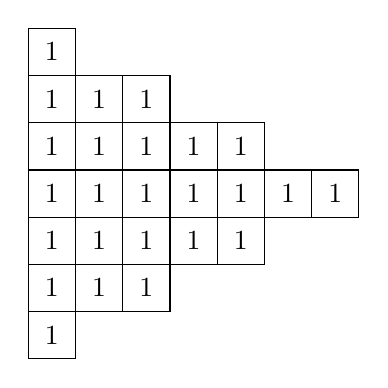
\begin{tikzpicture}[every node/.style={draw, minimum size=6mm, inner sep=0pt}]
  \foreach \col in {1}{
    \node at (\col*0.6, 6*0.6) {1};
  }
  \foreach \col in {1,2,3}{
    \node at (\col*0.6, 5*0.6) {1};
  }
  \foreach \col in {1,2,3,4,5}{
    \node at (\col*0.6, 4*0.6) {1};
  }
  \foreach \col in {1,2,3,4,5,6,7}{
    \node at (\col*0.6, 3*0.6) {1};
  }
  \foreach \col in {1,2,3,4,5}{
    \node at (\col*0.6, 2*0.6) {1};
  }
  \foreach \col in {1,2,3}{
    \node at (\col*0.6, 1*0.6) {1};
  }
  \foreach \col in {1}{
    \node at (\col*0.6, 0*0.6) {1};
  }
\end{tikzpicture}
\end{center}

\begin{enumerate}
  \item Using an array of pointers.
  \item Using a pointer to pointer.
\end{enumerate}
Free all dynamically allocated memory at the end of each program.
\mk{14} \yr{CSE 101 | L-1/T-1 | 2015--16}

%% Q32 — 2015-16 [Backlog]
\item Re-declare \texttt{double A[20][36][37]} using only pointers and \texttt{malloc()}. Do not use the \texttt{[]} operator.
\mk{7} \yr{CSE 101 | L-1/T-1 | 2015--16}

%% Q33 — 2018-19
\item Rewrite the following declaration using dynamic memory allocation to allocate an equivalent amount of memory:
 
\begin{lstlisting}
int matrix[NoRow][NoCol];
\end{lstlisting}
\mk{5} \yr{CSE 105 | L-1/T-2 | 2012--13}

%% Q29 — 2012-13
\item Consider a linked list based on the following structure:
\begin{lstlisting}
typedef struct { int month, day, year; } date;
typedef struct xx {
    char empID[10]; char name[30];
    char street[40]; char city[20];
    date birthdate; int salary;
    struct xx *next;
} record;
\end{lstlisting}
The first element is \texttt{start} and the last element is \texttt{NULL}. Write:
\begin{enumerate}
  \item A C function to display \texttt{empID}, \texttt{name}, and \texttt{city} of all employees whose salary is $\ge$ 20000, in tabular form.
  \item A C function to delete all employees from the list whose \texttt{city} is \texttt{"Khulna"}.
\end{enumerate}
\mk{20} \yr{CSE 105 | L-1/T-2 | 2012--13}

%% Q30 — 2015-16
\item Write a C program to read $n$ integers into an array and split it into two dynamically allocated arrays: one for even numbers and one for odd numbers. Allocate only as much memory as needed (no wasted memory).\\
\textit{Example:} Original: \texttt{7,9,4,6,5,3,2,10,18} $\to$ Odd: \texttt{7,9,5,3}; Even: \texttt{4,6,2,10,18}.
\mk{15} \yr{CSE 105 | L-1/T-2 | 2010--11}

%% Q26 — 2010-11
\item The following function is supposed to allocate memory for an integer array. Does it successfully allocate memory for variable \texttt{p} in \texttt{main}? Justify your answer.
 
\begin{lstlisting}
#include <stdlib.h>
void allocate(int t, int size) {
    t = (int)malloc(sizeof(int) * size);
}
int main() {
    int *p;
    allocate(p, 100);
}
\end{lstlisting}
\mk{7} \yr{CSE 105 | L-1/T-2 | 2010--11}

%% Q27 — 2010-11
\item Declare an array of 5 pointers to characters. Allocate exactly enough memory to store the strings \texttt{"Bangladesh"}, \texttt{"India"}, \texttt{"SriLanka"}, \texttt{"Nepal"}, and \texttt{"Bhutan"} (no extra memory). Show how you store the strings in the array.
\mk{10} \yr{CSE 105 | L-1/T-2 | 2010--11}

%% Q28 — 2012-13
\item
\begin{enumerate}
  \item Write a program that defines a triangular array with $n$ levels where level $i$ contains $i$ elements ($i = 1, 2, \ldots, n$). The value of $n$ is received as a command-line argument. Implement the array using pointer and dynamic memory allocation.
\begin{center}
      \begin{tikzpicture}[
        % Define standard square cell dimensions
        cell/.style={
            draw,
            minimum size=0.6cm,
            anchor=south west,
            inner sep=0pt
        }
    ]

    % ==========================================
    % DIAGRAM FOR n = 3
    % ==========================================
    
    % Label
    \node[font=\small] (label1) at (-0.8, 0.3) {$n=3$};
    
    % Bottom Row (3 blocks)
    \node[cell] (c3_11) at (0,0) {};
    \node[cell] (c3_12) at (0.6,0) {};
    \node[cell] (c3_13) at (1.2,0) {};
    
    % Middle Row (2 blocks)
    \node[cell] (c3_21) at (0,0.6) {};
    \node[cell] (c3_22) at (0.6,0.6) {};
    
    % Top Row (1 block)
    \node[cell] (c3_31) at (0,1.2) {};


    % ==========================================
    % DIAGRAM FOR n = 4
    % ==========================================
    \begin{scope}[xshift=4.5cm]
        % Label
        \node[font=\small] (label2) at (-0.8, 0.3) {$n=4$};
        
        % Bottom Row (4 blocks)
        \node[cell] (c4_11) at (0,0) {};
        \node[cell] (c4_12) at (0.6,0) {};
        \node[cell] (c4_13) at (1.2,0) {};
        \node[cell] (c4_14) at (1.8,0) {};
        
        % Second Row (3 blocks)
        \node[cell] (c4_21) at (0,0.6) {};
        \node[cell] (c4_22) at (0.6,0.6) {};
        \node[cell] (c4_23) at (1.2,0.6) {};
        
        % Third Row (2 blocks)
        \node[cell] (c4_31) at (0,1.2) {};
        \node[cell] (c4_32) at (0.6,1.2) {};
        
        % Top Row (1 block)
        \node[cell] (c4_41) at (0,1.8) {};
    \end{scope}

    \end{tikzpicture}
\end{center}
\mk{7} \yr{CSE 101 | L-1/T-2 | 2009--10}

%% Q20 — 2009-10
\item Write an insertion function for the triangular array above which inserts elements so that they become row- and column-wise sorted.
\mk{7} \yr{CSE 101 | L-1/T-2 | 2009--10}

%% Q21 — 2009-10
\item Write an efficient search function that searches an element in the triangular array and returns the row and column position as a \texttt{double} in the format \texttt{row.column} if present, or \texttt{-1.0} if absent.
\mk{7} \yr{CSE 101 | L-1/T-2 | 2009--10}

%% Q22 — 2009-10
\item Write a fetch function that retrieves a value from a given row and column position in the triangular array, or returns \texttt{-1.0} if the position is invalid.
\mk{7} \yr{CSE 101 | L-1/T-2 | 2009--10}
\end{enumerate}

%% Q23 — 2009-10
\item Consider the following declarations (doubly linked list):
\begin{lstlisting}
typedef struct { int month, day, year; } date;
typedef struct xx {
    char name[20]; char street[30]; char city[20];
    int acct_no; char acct_type;
    float oldbalance, newbalance, payment;
    date lastpayment;
    struct xx *next, *prev;
} record;
\end{lstlisting}
A doubly linked list has already been created. The first element is named \texttt{start}; the \texttt{prev} of \texttt{start} and the last element's \texttt{next} are both \texttt{NULL}. Write a C function to reorganize the records so that the list becomes sorted in ascending order of \texttt{acct\_no}.
\mk{25} \yr{CSE 101 | L-1/T-2 | 2009--10}\\
Write a C function to insert a new record in the sorted doubly linked list obtained from the previous question.
\mk{10} \yr{CSE 101 | L-1/T-2 | 2009--10}

%% Q25 — 2010-11
\item What is the purpose of using pointers in a C program? Consider the declaration \texttt{int **x;} Write necessary C code for memory allocation and initialization of \texttt{x} such that:
\[x[i][j] = \frac{2i}{3} + j(j-1) \quad \text{for } 0 \le i, j \le 10\]
\mk{10} \yr{CSE 101 | L-1/T-2 | 2008--09}


%% Q19 — 2009-10
\item Consider the declaration \texttt{int **pa;} Write necessary C code for memory allocation and initialization of \texttt{pa} such that \texttt{pa[i][j] = i*(i+1) + j/2} for $0 \le i \le 6$ and $0 \le j \le 5$.
\mk{8} \yr{CSE 105 | L-1/T-2 | 2007--08}

%% Q17 — 2008-09
\item Consider the following declaration:
\begin{lstlisting}
int **p;
\end{lstlisting}
Write C code for dynamic memory allocation so that \texttt{p} can point to a $10 \times 20$ table of integers (10 rows, 20 columns).
\mk{5} \yr{CSE 105 | L-1/T-2 | 2005--06}

%% Q16 — 2007-08
\item What is the problem with the following code fragments?
 
\begin{enumerate}
  \item \begin{lstlisting}
char *s;
s = (char *) malloc(100);
s = "hello";
free(s);
\end{lstlisting}
  \item \begin{lstlisting}
FILE *fp = fopen("file.dot", "r");
while (ch = getc(fp) != EOF)
    putc(stdout, ch);
\end{lstlisting}
\end{enumerate}
\mk{5} \yr{CSE 101N | L-1/T-1 | 2003--04}

%% Q11 — 2003-04
\item How can you know whether \texttt{malloc()} was successful in allocating memory? What is the purpose of the stack area in RAM?
\mk{5} \yr{CSE 101N | L-1/T-1 | 2003--04}

%% Q12 — 2003-04
\item Look at the following code where a function dynamically allocates memory for a pointer:
 
\begin{lstlisting}
void allocate(int *p, int n) {
    p = (int *) malloc(sizeof(int) * n);
    if (p == NULL) exit(0);
}
void main() {
    int *pa;
    allocate(pa, 10);
    pa[2] = 4;
}
\end{lstlisting}
What is the potential problem of using \texttt{allocate()} for pointer \texttt{pa}? Rewrite the function to fix the problem.
\mk{8} \yr{CSE 101N | L-1/T-1 | 2003--04}


%% Q15 — 2005-06
\end{enumerate}

%% ── S6: User-Defined Data Types ───────────────────────────────────────
\section{S6 --- User-Defined Data Types}
\label{sec:S6}
\markboth{S6 --- User-Defined Data Types}{}

%%──────────────────────────────────────────────────────────────────────
\subtopic{cC}{Structures}
\label{sub:s6-struct}

\begin{enumerate}

\item A two dimensional point has $x$ and $y$. Design a structure for that. Next, write a function that takes two variables of the structure type and returns the distance between the two points. Declare another structure with three members of the point structure type to store triangles. Next, write another function that takes a triangle structure as its parameter, and return the area of the triangle. You will use the pass by reference method to pass all structures to the respective functions.  
\mk{12} \yr{CSE 101 | L-1/T-1 | 2024--25}

%% Q8 — 2023-24
\item Consider a \texttt{struct studentstruct} defined with several fields (including at least one pointer or array field). Given:
 
\begin{lstlisting}
struct studentstruct { /* ... */ };
struct studentstruct a, b;
/* Taking input into a */
b = a; /* Copying a to b */
\end{lstlisting}
What problems may arise from such a direct struct assignment? What is the solution to make the copy correct (deep copy)?
\mk{8} \yr{CSE 101 | L-1/T-1 | 2023--24}

%% Q9 — 2022-23
\item Using a C program, define a structure named \texttt{Student} that includes attributes ID, name, and CGPA. Input an array of students from the user, sort them based on CGPA, and display the sorted list.
\mk{12} \yr{CSE 101 | L-1/T-1 | 2022--23}

%% Q10 — 2003-04
\item Implement the functions \texttt{createAccount}, \texttt{searchAccount}, \texttt{addBalance}, \texttt{transferBalance}, and \texttt{printTransactions} for a banking system with the following structure definitions:
\begin{lstlisting}
#include <stdio.h>
#include <string.h>
#include <time.h>

#define TOTAL_ACCOUNTS_AT_MOST 1000
#define TOTAL_TRANSACTIONS_AT_MOST 10000

typedef enum {
    SAVINGS,
    CURRENT
} AccountType;

typedef enum {
    WITHDRAW,
    DEPOSIT,
    TRANSFER
} TransactionType;

typedef struct {
    int date;
    int month;
    int year;
} Date;

typedef struct {
    Date date;
    int hour;
    int mins;
    int seconds;
} Time;

typedef struct {
    char *name;
    int accountNumber;
    int balance;
    AccountType type;
    Date dob;
    Time openingTime;
} Account;

typedef struct {
    Account *sentFrom;
    Account *sentTo;
    Time time;
    int amount;
    TransactionType type;
} Transaction;

Account* allAccounts[TOTAL_ACCOUNTS_AT_MOST];
Transaction* allTransactions[TOTAL_TRANSACTIONS_AT_MOST];

Time getCurrentTime();

// create an account and add the account to allAccounts array
// set account opening time by calling the function getCurrentTime
Account *createAccount(char *name, int accountNumber, int initialBalance, AccountType type, Date dob);

// search for the account number given.
Account *searchAccount(int accountNumber);

// add balance to an accountNumber. Add a transaction to the allTrasanctions array
void addBalance(int account, int amount);

// withdraw balance. Add a transaction to the allTrasanctions array
void withdrawBalance(int account, int amount);

// transfer balance from one account to another account. Add a transaction to the allTrasanctions array
void transferBalance(int from, int to, int amount);

// print all transactions of an account
void printTransactions(int account);
\end{lstlisting}
You cannot change any function prototypes.
\mk{25} \yr{CSE 101 | L-1/T-1 | 2021--22}

\item Look at the following C code:
 
\begin{lstlisting}
struct X { short s; int i; char c; };
struct Y { int i; short s; char c; };
struct Z { int i; char c; short s; };
const int sizeX = sizeof(struct X);
const int sizeY = sizeof(struct Y);
const int sizeZ = sizeof(struct Z);
int main() {
    printf("%d %d %d\n", sizeX, sizeY, sizeZ);
    return 0;
}
\end{lstlisting}
Write the output and provide a brief justification for each of \texttt{sizeX}, \texttt{sizeY}, and \texttt{sizeZ}. Assume \texttt{int}=4 bytes, \texttt{char}=1 byte, \texttt{short}=2 bytes.
\mk{15} \yr{CSE 101 | L-1/T-1 | 2020--21}

%% Q29 — 2021-22
\item Define a structure \texttt{District} to store year-long weather data about a district of Bangladesh. It should contain:
\begin{lstlisting}
Id (Integer identifier of district, between 1 and 64),
Temperature (An array of 365 real numbers),
Humidity (array of 365 real numbers),
Rain (An array of 365 real numbers). 
\end{lstlisting}
Declare an array named \texttt{districts} of type \texttt{District}.
\mk{10} \yr{CSE 101 | L-1/T-1 | 2019--20}

%% Q28 — 2020-21
\item Suppose we have a list of student names, identification numbers, and grades. For example, the beginning of the list might look like:
\begin{center}
    \ttfamily
    \begin{tabular}{lll}
        Casanova & 910017 & B \\
        Ayaan    & 934422 & A \\
        Smith    & 978766 & C \\
    \end{tabular}
\end{center}

Suppose there are five possible grades A, B, C, D, and F.

\begin{enumerate}
    \item[(i)] Write down a program called \texttt{recorder} that will perform the following tasks:
    
    Take the above data as input and put it into an array of structure. The number of students $N$ will also be input to your program first. Define your own structure. Assume that the names are single word names with max length of 50. The program should print out an ordered list of students and grades, i.e., students with A grades should be listed first, students with B grade next and so forth. Among all students having the same grade, the students should be listed alphabetically by name.
    
    \item[(ii)] Add a function \texttt{class\_average} to your program that will compute the class average and print it. Assume that A grade has value 4.0, a B grade has value 3.0, and so forth.
\end{enumerate}
\mk{20} \yr{CSE 101 | L-1/T-1 | 2018--19}

%% Q26 — 2018-19
\item Which of the two following structures consumes less memory? Show the calculation. Assume \texttt{int}=4 bytes, \texttt{char}=1 byte, \texttt{float}=4 bytes.
 
\begin{lstlisting}
struct A { char a; float d; char c; };
struct B { char a; char c; float d; };
\end{lstlisting}
\mk{5} \yr{CSE 101 | L-1/T-1 | 2018--19}

%% Q27 — 2019-20
\item The English Premier League (EPL) consists of 20 teams. Each team has a name,
    number of matches played, number of matches won, number of matches drawn, number
    of matches lost, total goals scored and total goals conceded.

    A sample data for 6 team is given below:

    \begin{center}
    \begin{tabular}{|l|c|c|c|c|c|c|}
    \hline
    \textbf{Name} & \textbf{Played} & \textbf{Win} & \textbf{Draw} & \textbf{Loss} & \textbf{Goals Scored} & \textbf{Goals Conceded} \\
    \hline
    Manchester United & 38 & 23 & 11 & 4  & 78 & 37 \\
    \hline
    Chelsea           & 38 & 21 & 9  & 8  & 69 & 33 \\
    \hline
    Manchester City   & 38 & 17 & 7  & 14 & 59 & 44 \\
    \hline
    Arsenal           & 38 & 19 & 11 & 8  & 72 & 43 \\
    \hline
    Liverpool         & 38 & 16 & 14 & 8  & 55 & 46 \\
    \hline
    Tottenham Hotspur & 38 & 21 & 8  & 9  & 60 & 33 \\
    \hline
    \end{tabular}
    \end{center}

    Now do the following:

    \begin{enumerate}
        \item[(i)] Define a C structure for a EPL team and necessary variables to work with 20 EPL
        teams.

        \item[(ii)] Write a function \texttt{\textbf{loadFromFile}} that loads all the club's information from a file
        \texttt{clubs.txt} to your program.

        \item[(iii)] Each club will get 3 points for a win, 1 point for a draw and no point for a loss.
        Based on this point scheme, write a function \texttt{\textbf{printPosition}} that prints each team's
        total point and their position. For example, the output for the above sample of 6 clubs
        will be as follows:

        \begin{center}
        \begin{tabular}{|l|c|c|}
        \hline
        \textbf{Name} & \textbf{Total Points} & \textbf{Position} \\
        \hline
        Manchester United & 80 & 1 \\
        \hline
        Chelsea           & 72 & 2 \\
        \hline
        Manchester City   & 58 & 6 \\
        \hline
        Arsenal           & 68 & 4 \\
        \hline
        Tottenham Hotspur & 71 & 3 \\
        \hline
        Liverpool         & 62 & 5 \\
        \hline
        \end{tabular}
        \end{center}

        \item[(iv)] Write a function \texttt{\textbf{storeToFile}} that sorts the above information based on ascending
        order of position and write to a file named \texttt{positions.txt}.
    \end{enumerate}

    \textbf{Note that, You can add parameters to the functions if necessary but you cannot
    hard code based on the sample data.}
\mk{18} \yr{CSE 101 | L-1/T-1 | 2015--16}

%% Q24 — 2015-16 [Backlog]
\item A hall management system records information of all students who are either resident
    or attached to that hall. The record has the following fields:

    \begin{center}
    \begin{tabular}{|l|l|}
    \hline
    \textbf{Fields} & \textbf{Description} \\
    \hline
    name       & Name of the student \\
    \hline
    stdID      & Student number \\
    \hline
    DoB        & Death of birth of the student \\
    \hline
    enrolDate  & Date of admission into the hall \\
    \hline
    Room No    & Room number of the residential student \\
    \hline
    GPA        & An array contains semester-wise GPA \\
    \hline
    \end{tabular}
    \end{center}

    \begin{enumerate}
        \item[(a)] Write down a suitable data structure to store the above mentioned information of all
        students associated with the hall. \mk{10}

        \item[(b)] Assume that \texttt{studentList} is a pointer to the list of all students as declared below:

        \texttt{Student *StudentList;}

        Write down a C function to list all the students (containing name, stdID and roomNo)
        whose CGPA is less than 3.0 and occupied seats in the hall.  \mk{10}

        Write a C function that will retrieve information of all students stored in the hard-disk
        into the variable \texttt{\textbf{studentList}} as declared in (b). At the end of the program, you are
        required to replace the information stored in the hard-disk with the information recorded
        in \texttt{\textbf{studentList}}, which is referred as \textbf{save} operation. Write another C function for \textbf{save}
        operation. Both of the function must be written in such a way that a student's information
        is considered as a single entity. (Hints: You are not allowed to use \texttt{fscanf()} or \texttt{fprintf()}
        functions in your program.) \mk{(8+7)}
    \end{enumerate}
 \yr{CSE 101 | L-1/T-1 | 2015--16}

\item You need to write some code for a banking system. In this system, there is a structure called \textit{AccoutBalance} to hold the account id (integer) and balance (double precision floating point). The structure is used to read account balance information from file and store in memory as needed, and vice versa. The total number of accounts is defined in a constant N. The accounts are identified by integers from 1 to $N$.

Today's opening balance information of all accounts is stored in a binary file called ``dayOpeningBalance.dat'' The file contains the data of the accounts in increasing order of account id. For each account, it stores an AccountBalance structure. Another binary file, called ``currentBalance.dat'' has the same format as the former file, but contains the current balance (instead of opening balance) for each account. Additionally, each transaction is logged into a text file called ``transactions.log''. In this file, each line contains an account id, followed by an amount (double precision floating point) that was added (positive number) to or deducted from (negative number) the account in a transaction. Obviously, there can be multiple transactions for an account in the log file.

\begin{enumerate}
    \item[(i)] Write the definition of \textit{AccountBalance} structure. What would be the size of it in bytes?
    
    \item[(ii)] Write a program that reads from console an account id, and outputs the opening and current balance of the corresponding account. For efficiency, you *must* use random access, instead of sequential access of the files. You may assume that the input account id is valid.
    
    \item[(iii)] In the above scenario, instead of reading the account id from console, read it as a command line argument and write necessary code to obtain the account id as an integer. (You don't need to rewrite the parts of reading/printing the balances)
    
    \item[(iv)] Write a program that processes all the recorded transactions to check that the current balance of each account is consistent, For example, if opening balance of account\# 1 is 4000 and there are 2 transactions in the log for account\# 1 which are ``1 2000'' and ``1 $-$ 1000'' then the current balance of the account must be 5000. For each account, your code should print the account id, followed by ``Account state is consistent state'' or ``Account state is inconsistent''.
\end{enumerate}
\mk{15} \yr{CSE 105 | L-1/T-2 | 2014--15}

%% Q23 — 2015-16
\item Write down an appropriate definition of a structure which has a \texttt{float} variable, an \texttt{int} variable, and a \texttt{char} variable. What will be the storage requirement? What will it be if you use a \texttt{union} instead?
\mk{8} \yr{CSE 105 | L-1/T-2 | 2011--12}

%% Q19 — 2011-12
\item Your friend has written the following program which gives no compiler error. However, your teacher says there is a problem. Identify it and suggest corrections:
 
\begin{lstlisting}
struct ADate { int month, day, year; };
int main(void) {
    struct ADate *d;
    d->month = 3;
    d->day   = 9;
    d->year  = 2014;
    return 0;
}
\end{lstlisting}
\mk{6} \yr{CSE 105 | L-1/T-2 | 2011--12}

%% Q20 — 2014-15
\item What is the \texttt{typedef} declaration? Give suitable examples.
\mk{5} \yr{CSE 105 | L-1/T-2 | 2010--11}

%% Q18 — 2011-12
\item Write down the following declarations:
\begin{enumerate}
  \item Define a structure consisting of two floating-point members called \texttt{real} and \texttt{imaginary}, with the tag \texttt{complex}.
  \item Declare a variable \texttt{x} of type \texttt{complex} and assign initial values 1.3 and $-$2.2 to \texttt{x.real} and \texttt{x.imaginary} respectively.
  \item Declare a pointer variable \texttt{px} which points to a structure of type \texttt{complex}. Write expressions for the structure members in terms of the pointer variable.
\end{enumerate}
\mk{13} \yr{CSE 101 | L-1/T-2 | 2009--10}

%% Q16 — 2009-10
\item Write a C program to solve the quadratic equation $ax^2 + bx + c = 0$ using the \texttt{complex} structure defined above. Display both real and imaginary roots and include all possible exceptions.
\mk{10} \yr{CSE 101 | L-1/T-2 | 2009--10}

%% Q17 — 2010-11
\item Define a self-referential structure containing the following members:
\begin{enumerate}
  \item A 40-element character array \texttt{name} and a 15-element character array \texttt{std\_id}.
  \item A date-type member \texttt{DOB} containing \texttt{day} (1--31), \texttt{month} (1--12), and \texttt{year} (1900--2100).
  \item Variables \texttt{m\_mark} and \texttt{p\_mark} for marks (0--100) in math and physics respectively; \texttt{m\_total} holds their sum.
  \item A pointer \texttt{next} to another structure of this same type.
\end{enumerate}
\mk{10} \yr{CSE 101 | L-1/T-2 | 2008--09}

%% Q15 — 2009-10
\item Suppose that the Chelsea football club has 30 players. Each player has several attributes: name, date of birth, country of citizenship, number of international appearances, salary (US\$ per week), and transfer fee from the previous club. Write C program code (not a complete program) to:
\begin{enumerate}
  \item Define structure(s) to store the information of these 30 players.
  \item Take input from the user to fill up these structures.
  \item Search and display the name of the most valuable player (in terms of transfer fees).
  \item Search and display the name of the youngest player.
\end{enumerate}
\mk{20} \yr{CSE 105 | L-1/T-2 | 2005--06}

%% Q13 — 2008-09
\item In geometry, a point is located by two coordinates $(x, y)$ and a circle is defined by its centre (a point) and a radius. Define two structures \texttt{Point} and \texttt{Circle}, and implement the following functions:
\begin{enumerate}
  \item \texttt{Circle makeCircle(Point p1, Point p2)} --- returns the circle where \texttt{p1} and \texttt{p2} are the endpoints of a diameter.
  \item \texttt{Point tangentPoint(Circle c1, Circle c2)} --- returns the point of tangency of two externally tangent circles.
\end{enumerate}

\begin{center}
  \begin{tabular}{cc}

    % --- Diagram (a) ---
    \begin{minipage}{0.45\textwidth}
    \centering
    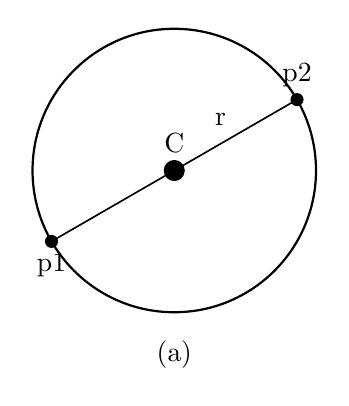
\begin{tikzpicture}[scale=1.8, >=stealth]
        % Draw main circle
        \draw[thick] (0,0) circle (1);
        
        % Define points for diameter
        \coordinate (C) at (0,0);
        \coordinate (P1) at (210:1);
        \coordinate (P2) at (30:1);
        
        % Draw diameter line
        \draw[semithick] (P1) -- (P2);
        
        % Draw and label center point C
        \filldraw[black] (C) circle (2pt) node[above=3pt] {C};
        
        % Draw and label boundary points
        \filldraw[black] (P1) circle (1.2pt) node[left=2pt, below=1pt] {p1};
        \filldraw[black] (P2) circle (1.2pt) node[right=2pt, above=1pt] {p2};
        
        % Label radius r
        \node at ($(C)!0.5!(P2)$) [above left] {r};
        
        % Subfigure label
        \node at (0,-1.3) {(a)};
    \end{tikzpicture}
    \end{minipage}

    &

    % --- Diagram (b) ---
    \begin{minipage}{0.5\textwidth}
    \centering
    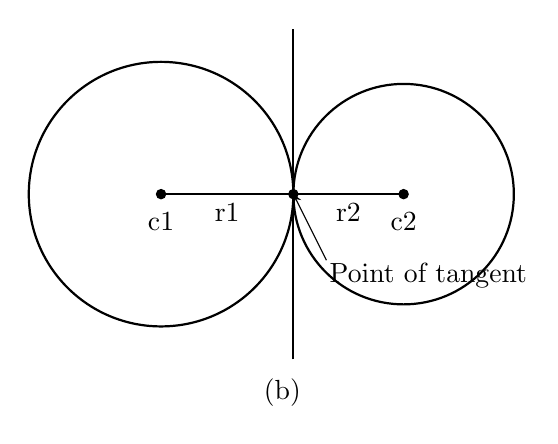
\begin{tikzpicture}[scale=1.4, >=stealth]
        % Define centers and radii
        \coordinate (C1) at (0,0);
        \coordinate (C2) at (2.2,0);
        
        % Draw circles
        \draw[thick] (C1) circle (1.2);
        \draw[thick] (C2) circle (1.0);
        
        % Draw centerline connection
        \draw[semithick] (C1) -- (C2);
        
        % Center points
        \filldraw[black] (C1) circle (1.2pt) node[below=3pt] {c1};
        \filldraw[black] (C2) circle (1.2pt) node[below=3pt] {c2};
        
        % Tangent line
        \coordinate (T) at (1.2, 0);
        \draw[thick] (1.2, -1.5) -- (1.2, 1.5);
        
        % Radius labels
        \node at (0.6, 0) [below] {r1};
        \node at (1.7, 0) [below] {r2};
        
        % Label pointer for Point of tangent
        \filldraw[black] (T) circle (1.2pt);
        \draw[<-] (T) -- (1.5, -0.6) node[below right, inner sep=1pt] {Point of tangent};
        
        % Subfigure label
        \node at (1.1,-1.8) {(b)};
    \end{tikzpicture}
    \end{minipage}

\end{tabular}
\end{center}
\mk{13} \yr{CSE 101N | L-1/T-1 | 2003--04}

%% Q11 — 2003-04
\item Show the output of the following code fragment:
 
\begin{lstlisting}
struct test {
    int x;
    int *y;
    int **z;
    struct test *p;
};
struct test bob;
bob.x   = 0;
bob.y   = &bob.x;
bob.z   = &bob.y;
bob.p   = &bob;
*bob.p->y  = 1;
**bob.p->z = 2;
printf("%d", bob.x);
\end{lstlisting}
\mk{6} \yr{CSE 101N | L-1/T-1 | 2003--04}

%% Q12 — 2005-06
\end{enumerate}

%%──────────────────────────────────────────────────────────────────────
\subtopic{cC}{Unions, Bit-fields \& Enumerations}
\label{sub:s6-union}

\begin{enumerate}

\item What is union data type? What is its role in memory conservation? Demonstrate the use of union and enumeration when the size of a T shirt is defined by strings like "S" (for small), "M" (for Medium), "L" (for large), "XL" (for extra Large) or the size of neck expressed by a fractional number. Illustrate the measures to be taken if you give input other than defined sizes.  
\mk{10} \yr{CSE 101 | L-1/T-1 | 2024--25}  

\item Explain the advantage of using enumeration data type and typedef in writing programs, with necessary examples.
\mk{8} \yr{CSE 101 | L-1/T-1 | 2024--25}  

%% Q6 — 2023-24
\item \textit{``Enumeration is used to save memory usage by computer programs''} --- justify this claim with necessary examples.
\mk{8} \yr{CSE 101 | L-1/T-1 | 2023--24}

%% Q7 — 2023-24
\item What is the \texttt{union} data type? What is its role in memory conservation? Demonstrate the use of a \texttt{union} when a student's result is identified by either a letter grade \textbf{or} a percentage of obtained marks.
\mk{10} \yr{CSE 101 | L-1/T-1 | 2023--24}

%% Q8 — 2003-04
\item Write the output of the following program:
 
\begin{lstlisting}
// sizeof: long double=16, float=4, int=4, char=1, char*=8
typedef union  { int i; char *ptr; float f; } example1;
typedef struct { char a; long double b; char *c; } example2;
typedef struct { long double b; char a; char *c; } example3;
typedef struct { char a[8]; int c; char b[8]; } example4;
int main() {
    printf("%ld\n", sizeof(example1));
    printf("%ld\n", sizeof(example2));
    printf("%ld\n", sizeof(example3));
    printf("%ld\n", sizeof(example4));
}
\end{lstlisting}
\mk{10} \yr{CSE 101 | L-1/T-1 | 2021--22}


\item Write the output of the following code snippet. Assume memory sharing starts from the least-significant bit.
 
\begin{lstlisting}
union test {
    unsigned int value  : 3;
    unsigned int value2 : 4;
};
int main() {
    union test t;
    printf("Sizeof(t) : %d\n", sizeof(t));
    t.value2 = 5;
    printf("t.value : %d, t.value2 : %d\n", t.value, t.value2);
    t.value2 = 9;
    printf("t.value : %d, t.value2 : %d\n", t.value, t.value2);
    t.value2 = 13;
    printf("t.value : %d, t.value2 : %d\n", t.value, t.value2);
}
\end{lstlisting}
\mk{15} \yr{CSE 101 | L-1/T-1 | 2020--21}

%% Q20 — 2020-21
\item BUET CSE identifies each student either by their nickname (a string of at most 10 characters) or by their student ID (an integer), but not both. Declare a data structure that allows storing this information for 120 students. Briefly explain why your chosen data structure is appropriate.
\mk{5} \yr{CSE 101 | L-1/T-1 | 2020--21}

%% Q21 — 2021-22
\item What is printed by the following program?
 
\begin{lstlisting}
struct test { unsigned a:1, b:2, c:3; };
int main() {
    int i;
    struct test x;
    for (i = 0; i < 8; ++i) {
        x.a = x.b = x.c = i;
        printf("%d %d %d\n", x.a, x.b, x.c);
    }
}
\end{lstlisting}
What happens if you replace \texttt{x.a = x.b = x.c = i;} with \texttt{x.c = x.b = x.a = i;}?
\mk{10} \yr{CSE 101 | L-1/T-1 | 2018--19}

%% Q19 — 2020-21
\item Define a bit-field structure called \texttt{Flags} consisting of: \texttt{flag\_1} (4 bits), \texttt{flag\_2} (2 bits), and \texttt{flag\_3} (2 bits). Write code to read values for those flags from the console.
\mk{5} \yr{CSE 105 | L-1/T-2 | 2014--15}


%% Q17 — 2014-15
\item Write a structure definition called \texttt{date} containing three bit-fields: \texttt{day} (5 bits), \texttt{month} (4 bits), and \texttt{year} (7 bits). Also write a union \texttt{identity} in which a \texttt{date} variable named \texttt{birthdate} shares the same memory location with an \texttt{int} variable called \texttt{slnumber}. Use \texttt{typedef} if necessary. How many decimal digits can \texttt{year} represent? Write a C function that reads \texttt{birthdate} as an integer, extracts \texttt{day}, \texttt{month}, and \texttt{year}, and prints the date in the form \texttt{dd-mm-yy}.
\mk{15} \yr{CSE 105 | L-1/T-2 | 2012--13}

%% Q16 — 2013-14
\item Discuss the use of a tagged union. Suppose you need to handle two types of students: one type receives marks in percentage (e.g.\ 90\%, 89.9\%), the other receives letter grades (e.g.\ A, A+). Use a tagged union to write a program that takes input for 5 students and displays their data.
\mk{15} \yr{CSE 105 | L-1/T-2 | 2011--12}

%% Q14 — 2011-12
\item Deduce the storage requirement of the variable \texttt{flag} below. State the range of values allowed for \texttt{f1} and \texttt{f2}:
 
\begin{lstlisting}
struct Flags {
    int          f1:3;
    unsigned int f2:1;
    unsigned int f3:30;
} flag;
\end{lstlisting}
\mk{6} \yr{CSE 105 | L-1/T-2 | 2011--12}

%% Q15 — 2012-13
\item Write a structure definition for the following situation: Define three bit-fields called \texttt{x}, \texttt{y}, and \texttt{z}, whose widths are 6 bits, 4 bits, and 6 bits respectively. Force \texttt{y} to begin at the start of a second 16-bit word. Separate \texttt{y} and \texttt{z} with 2 vacant bits. Declare a structure variable \texttt{v} and assign initial values 3, 5, and 7 to the three bit-fields. Show the graphical memory representation after assignment.
\mk{10} \yr{CSE 101 | L-1/T-2 | 2009--10}

%% Q12 — 2009-10
\item Define an enumeration type called \texttt{money} with the following members and values: \texttt{penny=1}, \texttt{nickel=5}, \texttt{dime=10}, \texttt{quarter=25}, \texttt{half=50}, \texttt{dollar=100}. Declare an enumeration variable \texttt{coins} of type \texttt{money} and assign it the initial value \texttt{dime}.
\mk{5} \yr{CSE 101 | L-1/T-2 | 2009--10}

%% Q13 — 2011-12
\item The data received from a network stream is stored in a byte (\texttt{unsigned char}) array, which can be interpreted as a list of variable-length records. The first byte of each record gives the data type as an ASCII character: \texttt{'C'} (char), \texttt{'S'} (short int), \texttt{'L'} (long int), \texttt{'F'} (float), \texttt{'D'} (double), or \texttt{'X'} (end of stream). The following bytes store a data item of that type. Provide definitions for:
\begin{enumerate}
  \item \texttt{void printStreamPtr(unsigned char *stream);} --- print each data item on a separate line using a \texttt{void *} pointer.
  \item \texttt{void printStreamUnion(unsigned char *stream);} --- print each data item on a separate line using a \texttt{struct} or \texttt{union} pointer.
\end{enumerate}
\mk{16} \yr{CSE 101 | L-1/T-2 | 2008--09}

%% Q11 — 2009-10
\item What is the basic difference between a structure and a union?
\mk{5} \yr{CSE 105 | L-1/T-2 | 2005--06}

%% Q10 — 2008-09
\item What are the advantages of using enumeration variables over using \texttt{\#define} within a program? Summarise the rules for assigning numerical values to enumeration constants with a suitable example.
\mk{5} \yr{CSE 101N | L-1/T-1 | 2003--04}

%% Q9 — 2005-06
\end{enumerate}

%% ══════════════════════════════════════════════════════════════════════
%%  PART IV — I/O, BITWISE, PREPROCESSORS & MISCELLANEOUS
%% ══════════════════════════════════════════════════════════════════════
\secdivider{Part IV}{I/O, Bitwise, Preprocessors \& Miscellaneous}{cD}{cD}

%% ── S7: Input/Output ──────────────────────────────────────────────────
\section{S7 --- Input/Output}
\label{sec:S7}
\markboth{S7 --- Input/Output}{}

%%──────────────────────────────────────────────────────────────────────
\subtopic{cD}{Console \& Formatted I/O}
\label{sub:s7-consoleio}

\begin{enumerate}

%% Q6 — 2005-06
\item Explain the file opening modes \texttt{"r"}, \texttt{"w"}, \texttt{"a"}, \texttt{"r+"}, \texttt{"w+"}, and \texttt{"a+"}.
\mk{6} \yr{CSE 101 | L-1/T-1 | 2021--22}

\item Some program codes are given below:
 
\begin{lstlisting}
int a = 0x7c5;
float x = 13.25;
printf("%-07X %#7g %10.2e", a, x, x);
\end{lstlisting}
Show the output generated by the \texttt{printf()} call. Also show the bit-stream stored in memory when storing 13.25 using the 4-byte IEEE 754 floating-point representation. Show your working.
\mk{13} \yr{CSE 101 | L-1/T-1 | 2020--21}

%% Q11 — 2021-22
\item A C program contains the following variable declarations:
\begin{lstlisting}
float a = 2.5, b = 0.0005, c = 3000;
\end{lstlisting}
Show and explain the output of:
\begin{lstlisting}
printf("%8.3f %-3e %#8f", a, b, c);
\end{lstlisting}
\mk{6} \yr{CSE 101 | L-1/T-2 | 2008--09}

%% Q10 — 2020-21
\item The date of September 5, 1979 is written in different forms: \texttt{05/09/1979}, \texttt{05-09-1979}, and \texttt{05.09.1979}. Write C code that can take a date as input in any of these three forms using a single \texttt{scanf()} function call.
\mk{5} \yr{CSE 105 | L-1/T-2 | 2005--06}

%% Q7 — 2005-06
\item Write down a \texttt{scanf()} function call statement that takes a string terminated by a newline character as input.
\mk{5} \yr{CSE 105 | L-1/T-2 | 2005--06}

%% Q8 — 2005-06
\item Explain the following statements where \texttt{var} is a character array containing 50 elements:
\begin{enumerate}
  \item \texttt{scanf("\%s", var);}
  \item \texttt{scanf("\%s", \&var);}
  \item \texttt{scanf("\%s", \&var[0]);}
\end{enumerate}
\mk{9} \yr{CSE 105 | L-1/T-2 | 2005--06}

%% Q9 — 2008-09
\end{enumerate}

%%──────────────────────────────────────────────────────────────────────
\subtopic{cD}{File I/O \& Command Line Arguments}
\label{sub:s7-fileio}

\begin{enumerate}


\item Explain the necessity of the file opening modes specified by "r+", "w+" and "a+" by briefly describing the scenarios.
\mk{6} \yr{CSE 101 | L-1/T-1 | 2024--25}

\item Read line by line from two text files and check whether they match. Stop when you get the first mismatch and display the two mismatched lines.
\mk{10} \yr{CSE 101 | L-1/T-1 | 2024--25}


%% Q7 — 2023-24
\item Explain the file opening modes \texttt{"r"}, \texttt{"w"}, \texttt{"a"}, \texttt{"r+"}, \texttt{"w+"}, and \texttt{"a+"} in C's \texttt{fopen}.
\mk{6} \yr{CSE 101 | L-1/T-1 | 2023--24}

%% Q8 — 2023-24
\item You are to manage the marks of $m$ subjects for a number of students using a file. Write a program that:
\begin{enumerate}
  \item Takes $m$ subject marks and a student ID, and stores them in a file (data persists after program exit).
  \item Given a student ID, retrieves and displays that student's marks.
  \item Outputs the total marks for each student and the highest mark for each subject.
\end{enumerate}
\mk{13} \yr{CSE 101 | L-1/T-1 | 2023--24}

%% Q9 — 2022-23
\item Develop a C program that retrieves two numbers from command line arguments, calculates their sum, and displays the result. You may use any library function.
\mk{12} \yr{CSE 101 | L-1/T-1 | 2022--23}

%% Q10 — 2022-23
\item Suppose you have a file containing the following contents (one integer per line): 185, 170, 165, 178, 167, 137, 156. Write a C program to read this file and sum up all the \textbf{odd} numbers. The file path is passed as a command line argument.
\mk{11} \yr{CSE 101 | L-1/T-1 | 2022--23}

%% Q11 — 2003-04
\item The following code reads 10 integers from a file and writes their sum at the end. Make any necessary corrections:
 
\begin{lstlisting}
FILE *fp = fopen("input.txt", "r");
int num = 0, sum = 0;
for (int i = 0; i < 10; i++) {
    fscanf(fp, "%d", &num);
    sum += num;
}
fprintf(fp, "%d", sum);
\end{lstlisting}
\mk{4} \yr{CSE 101 | L-1/T-1 | 2021--22}

%% Q42 — 2021-22
\item Write a program that creates a new file containing the contents of a given text file written twice. If the input file contains \texttt{"Dhaka is the capital of Bangladesh"}, the output file should contain that line twice.
\mk{10} \yr{CSE 101 | L-1/T-1 | 2021--22}

%% Q43 — 2021-22
\item Take marks for 10 students in 5 subjects as input. Find and display the names and total marks of the students with the highest and lowest totals. You are not allowed to use arrays to store marks or names --- use files instead.
\mk{15} \yr{CSE 101 | L-1/T-1 | 2021--22}

\item Read from \texttt{in.txt} until EOF. Each line contains a string and a number. For each line, determine (i) whether the string is a palindrome, and (ii) whether the number is odd or even. Write one output line per input line to \texttt{out.txt}.\\
\textit{Example in.txt:} \texttt{ABED 21 / ABSBA 23 / NIBIR 26}\\
\textit{Example out.txt:} \texttt{Not-Palindrome Odd / Palindrome Odd / Not-Palindrome Even}
\mk{15} \yr{CSE 101 | L-1/T-1 | 2020--21}

%% Q41 — 2021-22
\item Define a structure \texttt{District} to store year-long weather data about a district of Bangladesh. It should contain:
\begin{lstlisting}
Id (Integer identifier of district, between 1 and 64),
Temperature (An array of 365 real numbers),
Humidity (array of 365 real numbers),
Rain (An array of 365 real numbers). 
\end{lstlisting}
Declare an array named \texttt{districts} of type \texttt{District}.\\

A file \texttt{data.txt} contains daily weather data in the format: \texttt{<district\_id> <day> <temperature> <humidity> <rain>}. Information for 365 days is available for all 64 districts (not necessarily in order). Process all lines and for each weather attribute (temperature, humidity, rain), create a file named after the attribute. Each line of that file should contain a district's ID followed by its average attribute value across 365 days (district \#1 first, district \#64 last).
\mk{20} \yr{CSE 101 | L-1/T-1 | 2019--20}

%% Q38 — 2019-20
\item Write a program to copy the content of a file to another file using command-line arguments for the source and destination filenames. Handle errors related to file operations and command-line argument processing.
\mk{10} \yr{CSE 101 | L-1/T-1 | 2019--20}

%% Q39 — 2019-20
\item A binary file represents an image: the first 2 integers are height $h$ and width $w$; then $h \times w$ pixel values in RGBA model (row-major order). Some pixels are corrupted. Read from console: the image filename and the number of erroneous pixels. For each erroneous pixel, read its row, column (0-based), and the correct value. Use random access to update only the faulty pixels (do not unnecessarily read/write other pixels).
\mk{20} \yr{CSE 101 | L-1/T-1 | 2019--20}

%% Q40 — 2020-21
\item Write a program that clones itself in reverse: copy the source file's content in reverse order and save the copy as \texttt{rcopy.c}.
\mk{10} \yr{CSE 101 | L-1/T-1 | 2018--19}

%% Q37 — 2019-20
\item Write a C program to find the length of a file in bytes without reading the whole file.
\mk{6} \yr{CSE 101 | L-1/T-1 | 2015--16}

%% Q35 — 2015-16
\item Write a C program that takes a series of integer inputs from the command line and prints the maximum and minimum. For example: \texttt{5c.exe 3 7 9 -1 5 7 9 10} prints 10 as maximum and $-1$ as minimum.
\mk{7} \yr{CSE 101 | L-1/T-1 | 2015--16}

%% Q36 — 2018-19
\item Using the \texttt{AccountBalance} structure, write a program that reads an account ID as a command-line argument (as an integer). (You do not need to rewrite the balance reading/printing code.)
\mk{5} \yr{CSE 105 | L-1/T-2 | 2014--15}

%% Q34 — 2015-16
\item Write a C program that accepts a file name as a command-line argument and prints the contents of the file to a printer. If no file name is provided on the command line, the program asks for the file name from standard input, then prints the file's contents to a printer.
\mk{15} \yr{CSE 105 | L-1/T-2 | 2013--14}

\item Write a C program that accepts two filenames as command line parameters and
appends the second file to the first. If the user forgets to provide one or both filenames
while running the program from the command line, the program will ask for and read the
filename(s) accordingly .
\mk{15} \yr{CSE 105 | L-1/T-2 | 2012--13}

\item Discuss the formats and differences between read() and fread() functions.
\mk{5} \yr{CSE 105 | L-1/T-2 | 2012--13}

%% Q33 — 2014-15
\item Explain the purpose and semantic meaning of the following C function using necessary figures:
 
\begin{lstlisting}
int main(int argc, char **argv) {
    while (--argc > 0 && (*++argv)[0] == '-')
        while (c = *++argv[0])
            printf("%c\n", c);
}
\end{lstlisting}
\mk{10} \yr{CSE 101 | L-1/T-2 | 2012--13, 2009--10, 2008--09}

%% Q32 — 2013-14
\item Write a program named \texttt{myCopy} that copies the contents of one file to another. Command-line behaviour: two filenames $\to$ first is source, second is destination; one filename $\to$ it is the source, prompt for destination; no filenames $\to$ prompt for both. In case of any error opening either file, inform the user and ask for another filename.
\mk{22} \yr{CSE 105 | L-1/T-2 | 2011--12}

%% Q30 — 2011-12
\item You want to open an existing file for both read and write operations. Your friend says you can use \texttt{'r+'}, \texttt{'w+'}, or \texttt{'a+'} as the mode. Do you agree? Justify your answer.
\mk{7} \yr{CSE 105 | L-1/T-2 | 2011--12}

%% Q31 — 2012-13
\item Write a program that takes a file name as input and counts the total number of lines in the file. Lines end with a newline character. The program should handle errors such as a file not found.
\mk{12} \yr{CSE 105 | L-1/T-2 | 2010--11}

%% Q27 — 2010-11
\item Write a program that takes a number of command-line arguments (all integers) and finds the median and mode. Sort the numbers to find the median (middle element; average of two middle elements if even count). The mode is the most frequently occurring number; print \texttt{"No Mode"} if no number appears more than once.\\
\textit{Sample:} \texttt{\{4,1,1,10,3,5,7\}} $\to$ median=4, mode=1; \quad \texttt{\{2,1,4,7\}} $\to$ median=3, mode=No Mode.
\mk{20} \yr{CSE 105 | L-1/T-2 | 2010--11}

%% Q28 — 2010-11
\item
\begin{enumerate}
  \item Complete the following structure definition by declaring fields for book title (at most 99 chars), author name (at most 49 chars), and price (a real number):
\begin{lstlisting}
struct Bookinfo {
    /* title, author, price */
};
\end{lstlisting}
  \item Using the above structure, write a \texttt{main} program that reads info for 10 books and stores them in \texttt{"bookinfo.bin"} using \texttt{fwrite}.
  \item Write another program that asks for a book title, searches \texttt{"bookinfo.bin"} using \texttt{fread}, and prints the price. Print \texttt{"Sorry, we do not have the book"} if not found.
\end{enumerate}
\mk{25} \yr{CSE 105 | L-1/T-2 | 2010--11}

%% Q29 — 2011-12
\item A data structure has fields: \texttt{name} (80 chars), \texttt{address} (100 chars), and \texttt{date\_of\_birth} of a type defined as:
\begin{lstlisting}
typedef struct {
    unsigned month : 4;
    unsigned day   : 5;
    unsigned year  : 7;
} date;
\end{lstlisting}
The file \texttt{"data.old"} contains records. Write a C function that creates a new file \texttt{"data.new"} and copies all information from \texttt{"data.old"}, transferring one person's data at a time.
\mk{10} \yr{CSE 101 | L-1/T-2 | 2009--10}

%% Q24 — 2009-10
\item The skeletal outline of a C program is shown. Write the necessary program code to: (i) read the string \texttt{name} from \texttt{sample.old}; (ii) display it on screen; (iii) accept an updated string; (iv) write the new string to \texttt{sample.new}.
 
\begin{lstlisting}
#include <stdio.h>
main() {
    FILE *pt1, *pt2;
    char name[80];
    pt1 = fopen("sample.old", "r");
    pt2 = fopen("sample.new", "w");
    /* ... your code ... */
    fclose(pt1); fclose(pt2);
}
\end{lstlisting}
\mk{12} \yr{CSE 101 | L-1/T-2 | 2009--10}



%% Q23 — 2009-10
\item Write a program that takes one or more command-line options followed by a keyword and performs the following:
\begin{enumerate}
  \item \texttt{-l} : print the keyword in lower case
  \item \texttt{-u} : print the keyword in upper case
  \item \texttt{-t} : toggle the case of each alphabetic character in the keyword
  \item \texttt{-n} : print the number of characters in the keyword
\end{enumerate}
Options start with \texttt{-}. Multiple options may be grouped (e.g.\ \texttt{-uln} is equivalent to \texttt{-u -l -n}). Access command line arguments using pointer operations.
\mk{17} \yr{CSE 105 | L-1/T-2 | 2007--08}

%% Q19 — 2007-08
\item Write a function prototyped as \texttt{void concat\_file(char f1[], char f2[], char f3[])} which concatenates files \texttt{f1} and \texttt{f2} into file \texttt{f3}.
\mk{10} \yr{CSE 105 | L-1/T-2 | 2007--08}

%% Q20 — 2007-08
\item What are the differences between a text file and a binary file? Write a function that finds the size of a file.
\mk{15} \yr{CSE 105 | L-1/T-2 | 2007--08}

%% Q21 — 2008-09
\item The popular DX-BALL game shows high scores for the top 10 scorers in sorted order. Implement a similar system using a random-access file. Define an appropriate structure to store high scores (player name and score). Take 10 high scores as input, sort them in non-descending order, and store the sorted records in a random-access file.
\mk{20} \yr{CSE 105 | L-1/T-2 | 2005--06}

%% Q17 — 2005-06
\item Write C code that opens a file \texttt{"a.txt"} in read mode and another file \texttt{"b.txt"} in write mode, then copies only the vowel letters from \texttt{"a.txt"} to \texttt{"b.txt"}.
\mk{10} \yr{CSE 105 | L-1/T-2 | 2005--06}

%% Q18 — 2007-08
\item Write a program that compares two text files, printing the \textbf{first line} where they differ.
\mk{10} \yr{CSE 101N | L-1/T-1 | 2003--04}

%% Q12 — 2003-04
\item What are the differences between text files and binary files? Which is more efficient for storing data and why?
\mk{5} \yr{CSE 101N | L-1/T-1 | 2003--04}

%% Q13 — 2003-04
\item Write a program that reads data from a text file \texttt{"employee.txt"} where each line has the format:\\
Each line will contain the name of an employee, followed by a tab, followed by the number of hours worked, followed by a tab, followed by the hourly pay rate, followed by a newline. For example, the file looks like the following:\\
\begin{lstlisting}
Zahed Khan<tab>45<tab>20.00<newline>
Abdur Rahman<tab>32<tab>30.50<newline>
\end{lstlisting}
For each employee, compute and print their total pay (hours $\times$ rate). Handle the case of overtime (hours $>$ 40) if applicable.
\mk{8} \yr{CSE 101N | L-1/T-1 | 2003--04}

%% Q14 — 2003-04
\item What are the four parameters of the \texttt{fread()} function? Explain each.
\mk{4} \yr{CSE 101N | L-1/T-1 | 2003--04}

%% Q15 — 2003-04
\item An anonymous hacker wants to garble a file \texttt{"exam-ques101.doc"} (size $> 200$ bytes) by swapping its first 100 bytes with its last 100 bytes. Write a program fragment that performs this task using \texttt{fseek}, \texttt{fread}, and \texttt{fwrite}.
\begin{center}
   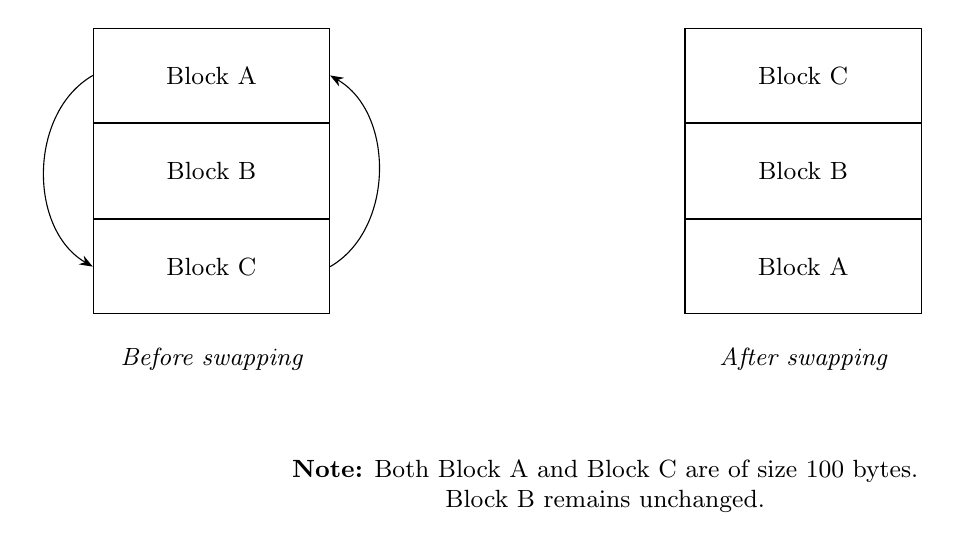
\begin{tikzpicture}[
        % Style for the individual memory sub-blocks
        block/.style={
            draw, 
            minimum width=3cm, 
            minimum height=1.2cm, 
            text centered, 
            font=\small
        },
        >=Stealth,
        node distance=0cm % Stack blocks directly on top of each other
    ]

    % ==========================================
    % BEFORE SWAPPING DIAGRAM
    % ==========================================
    
    % Base stack nodes
    \node[block] (B_before) {Block B};
    \node[block, above=of B_before] (A_before) {Block A};
    \node[block, below=of B_before] (C_before) {Block C};
    
    % Curved swapping arrows
    % Left arrow: A to C
    \draw[->] (A_before.west) to[out=210, in=150] (C_before.west);
    % Right arrow: C to A
    \draw[->] (C_before.east) to[out=30, in=330] (A_before.east);
    
    % Subtext label
    \node[below=0.3cm of C_before, font=\itshape\small] (label1) {Before swapping};


    % ==========================================
    % AFTER SWAPPING DIAGRAM
    % ==========================================
    
    % Position the second stack 4.5cm to the right of the first one
    \node[block, right=4.5cm of B_before] (B_after) {Block B};
    \node[block, above=of B_after] (C_after) {Block C};
    \node[block, below=of B_after] (A_after) {Block A};
    
    % Subtext label
    \node[below=0.3cm of A_after, font=\itshape\small] (label2) {After swapping};


    % ==========================================
    % FOOTNOTE / NOTE SECTION
    % ==========================================
    \node[font=\small, align=center] at ( 5,-4) {
        \textbf{Note:} Both Block A and Block C are of size 100 bytes.\\
        Block B remains unchanged.
    };

    \end{tikzpicture}
\end{center}

\mk{10} \yr{CSE 101N | L-1/T-1 | 2003--04}

%% Q16 — 2005-06
\end{enumerate}

%%──────────────────────────────────────────────────────────────────────
%% ── S8: Bitwise Operations ────────────────────────────────────────────
\section{S8 --- Bitwise Operations}
\label{sec:S8}
\markboth{S8 --- Bitwise Operations}{}

%%──────────────────────────────────────────────────────────────────────
\subtopic{cD}{Bitwise Operators \& Applications}
\label{sub:s8-bitwise}

\begin{enumerate}

\item Write down a function that will determine whether a number $x$ given as parameters can be expressed as $2^n$ or not, for any integer $n \geq 0$. Function shall return 1 if so, and shall return zero otherwise. You cannot use any library function to solve the problem.
\mk{10} \yr{CSE 101 | L-1/T-1 | 2024--25}

\item Write the following four functions using bitwise operators. You must maintain the restrictions mentioned in the 'restriction' column in the table.
    
   \begin{center}
    \begin{tabular}{|p{4.5cm}|p{4.5cm}|p{4.5cm}|}
        \hline
        \textbf{Function prototype} & \centering\textbf{Description} & \textbf{Restrictions} \\ \hline
        \texttt{int isNotEqual(int x, int y);} & Compares \texttt{x} and \texttt{y} for inequality. It should return 1 if the tested condition holds and 0 otherwise. & You cannot use \underline{\texttt{if-else}}, \underline{logical}, \underline{relational} or \underline{ternary} operator. You can only use \underline{bitwise} operators. \\ \hline
        \texttt{int copyLSB(int x);} & Set all bits of \texttt{x} same to least significant bit of \texttt{x} & You cannot use \underline{\texttt{if-else}}, \underline{logical}, \underline{relational} or \underline{ternary} operator. You can only use \underline{bitwise} operators. \\ \hline
        \texttt{int bitCount(int x);} & Returns a count of the number of 1's in the argument. & No restrictions. \\ \hline
        \texttt{int xtractRight(int x, int n);} & Returns rightmost n bits of the integer x. Assume $1 \leq n \leq 32$ & No restrictions. \\ \hline
    \end{tabular}
  \end{center}
\mk{20} \yr{CSE 101 | L-1/T-1 | 2024--25}


\item Consider the following program fragment which was written to find second largest of three numbers given as input. The variable \textit{secondL} is supposed to hold the second largest of three numbers. Complete the statement in Line 7 below using \underline{only} bitwise operators so that it correctly assigns second largest of three numbers to s.
\begin{lstlisting}
int a, b, c, max, min, s;
scanf("%d%d%d", &a, &b, &c);
max = (a > b ? a : b);
max = (max < c ? c : max);
min = (a < b ? a : b);
min = (min > c ? c : min);
secondL = 
printf("Second Largest", s);
\end{lstlisting}
\mk{5} \yr{CSE 101 | L-1/T-1 | 2024--25}

  %% Q13 — 2023-24
\item Write a function \texttt{int allRepeated(int x)} that returns 1 if and only if the positive integer \texttt{x} consists \textbf{only} of pairs of repeated digits, and 0 otherwise. You \textbf{must} use the XOR operator (5 marks deducted otherwise). Examples:
\begin{center}\small
\begin{tabular}{|l|c|}
\hline
\textbf{Function call} & \textbf{Return} \\ \hline
\texttt{allRepeated(7)}     & 0 \\ \hline
\texttt{allRepeated(77)}    & 1 \\ \hline
\texttt{allRepeated(7733)}  & 1 \\ \hline
\texttt{allRepeated(777)}   & 0 \\ \hline
\texttt{allRepeated(7777)}  & 1 \\ \hline
\texttt{allRepeated(2323)}  & 0 \\ \hline
\texttt{allRepeated(22332)} & 0 \\ \hline
\end{tabular}
\end{center}
\mk{20/15} \yr{CSE 101 | L-1/T-1 | 2023--24}
\yr{CSE 105 | L-1/T-2 | 2012--13}

%% Q7 — 2023-24
\item Write a function \texttt{int countMinBits(int n)} that counts and returns the minimum number of bits required to represent the integer $n$. You \textbf{must} use bitwise operators.
\mk{15} \yr{CSE 101 | L-1/T-1 | 2023--24}

%% Q8 — 2023-24
\item Write a function \texttt{int findTrailingZeros(int n)} that finds and returns the total number of trailing zeros in the binary representation of the integer $n$. You \textbf{must} use bitwise operators.
\mk{15} \yr{CSE 101 | L-1/T-1 | 2023--24}

%% Q9 — 2022-23
\item Write the following four functions in C conforming to the restrictions listed beside each:
\begin{center}
  \renewcommand{\arraystretch}{1.4} 
\begin{tabularx}{\textwidth}{|l|X|X|}
\hline
\textbf{Function Name} & \textbf{Description} & \textbf{Restrictions} \\ \hline
\texttt{negate(x)} & returns \texttt{-x} & Legal operators: \texttt{\textasciitilde{} +} \\ \hline
\texttt{isNotEqual(x,y)} & Compares \texttt{x} to \texttt{y} for inequality. It should return 1 if the tested condition holds and 0 otherwise. & Legal operators: \texttt{! \textasciitilde{} \& \textasciicircum{} \textbar{} << >>} \newline You cannot use any loop/recursion. \\ \hline
\texttt{copyLSB(x)} & Replicates a copy of the least significant bit in all 32 bits of the result. & Legal operators: \texttt{! \textasciitilde{} \& \textasciicircum{} \textbar{} << >>} \newline You cannot use any loop/recursion. \\ \hline
\texttt{isPositive(x)} & Return 1 if \texttt{x > 0}, return 0 otherwise & Legal operators: \texttt{! \textasciitilde{} \& \textasciicircum{} \textbar{} << >>} \newline You cannot use any loop/recursion. \\ \hline
\end{tabularx}
\end{center}
\mk{16} \yr{CSE 101 | L-1/T-1 | 2022--23}

%% Q10 — 2022-23
\item Write a C program that inputs two integers and determines how many bits they have \textbf{in common} (same bit value at the same position). For instance, $-1$ and $1$ have exactly one bit in common; 201 and 32767 have 21 bits in common.

\begin{lstlisting}
+1 =0000 0000 0000 0000 0000 0000 0000 0001
-1 =1111 1111 1111 1111 1111 1111 1111 1111
\end{lstlisting}
\begin{lstlisting}
  201=0000 0000 0000 0000 0000 0000 1100 1001
32767=0000 0000 0000 0000 0111 1111 1111 1111
\end{lstlisting}

\mk{12} \yr{CSE 101 | L-1/T-1 | 2022--23}
    
\item Answer the questions below for the given program (Listing 8):

\begin{lstlisting}
#include <stdio.h>

// print the bits of integer x (assume little endian machine)
void printBits(int x);

// set the bit at position p
int setBit(int x, int p);

// clear the bit at position p
int clearBit(int x, int p);

// invert the bit at position p
int invertBit(int x, int p);

// set left n bits starting from position p
int setBits(int x, int p, int n);

// clear left n bits starting from position p
int clearBits(int x, int p, int n);

// invert left n bits starting from position p
int invertBits(int x, int p, int n);

// right circular shift by n bits
int rightCircularShift(int x, int n);

// left circular shift by n bits
int leftCircularShift(int x, int n);

int setDefaultSystemStatus(int x)
{
    // x has a total of 32 bits
    // the first 16 bits are used for storing the os status
    // the next 12 bits are used for storing the total number of running processes
    // the next 3 bits are used for the error status
    // the last bit is unused

    // setting the os status to 0xff11 (1111111100010001)
    x = clearBits(x, 0, 16);
    x = setBit(x, 0);
    x = setBit(x, 4);
    x = setBits(x, 8, 8);

    // setting the total number of processes to 0xf43 (111101000011)
    x = clearBits(x, 16, 12);
    x = setBits(x, 16, 2);
    x = setBit(x, 22);
    x = setBits(x, 24, 4);

    // setting the error status to 0x6 (110)
    x = clearBits(x, 28, 3);
    x = setBits(x, 29, 2);

    return x;
}

int main()
{
    int x;
    // x has a total of 32 bits
    // the first 16 bits are used for storing the os status
    // the next 12 bits are used for storing the total number of running processes
    // the next 3 bits are used for the error status
    // the last bit is unused
    x = setDefaultSystemStatus(x);
    printBits(x);
}
\end{lstlisting}

    \begin{enumerate}
        \item[(a)] Implement the following functions: (You cannot change any function prototypes and follow the instructions given in the comments. You must use bit manipulation techniques and cannot use any loops and cannot include any libraries).
        \begin{enumerate}
            \item[(i)] \texttt{printBits} \hfill \mk{(4)}
            \item[(ii)] \texttt{setBit}, \texttt{clearBit}, and \texttt{invertBit} \hfill \mk{(2$\times$3=6)}
            \item[(iii)] \texttt{setBits}, \texttt{clearBits}, and \texttt{invertBits} \hfill \mk{(3$\times$3=9)}
            \item[(iv)] \texttt{rightCircularShift}, and \texttt{leftCircularShift} \hfill \mk{(3+3=6)}
        \end{enumerate}
        
        \item[(b)] Write a new program where you must implement the functionalities of the \texttt{setDefaultSystemStatus} function using Bit Field Structure. Note that you cannot use any bit manipulation technique in this program. \hfill \mk{10}
    \end{enumerate}
\yr{CSE 101 | L-1/T-1 | 2021--22}

\item Upon getting admission into BUET, a student gets a student ID comprising 7 digits. The first two digits are used for representing year, the next two digits for dept code and the last three digits for serial number as shown below: 

\begin{center}
    \renewcommand{\arraystretch}{1.2}
    \begin{tabular}{|c|c|c|c|c|c|c|}
        \hline
        \multicolumn{2}{|c|}{Year} & \multicolumn{2}{c|}{Dept Code} & \multicolumn{3}{c|}{Serial number} \\ \hline
        ~~~~2~~~~ & ~~~~0~~~~ & ~~~~0~~~~ & ~~~~5~~~~ & ~~~~4~~~~ & ~~~~5~~~~ & ~~~~6~~~~ \\ \hline
    \end{tabular}
\end{center}

\noindent
Consider that the program uses student ID for interface i.e., input and output purposes but use a student code for storing it inside computer memory. The 2 digits year in student ID is converted into 4 digits in student code. For example, if the year in student ID is 20, then it is converted to 2020 in student code. 4-byte integer variables are used for representing both the student ID and the student code. The most significant 1 bit, i.e., sign bit of student code is kept unused and always contains zero. The numbers of bits used for representing Year, Dept code and Serial number in student code are 13, 9 and 9, respectively, as showing below-

\begin{center}
    \renewcommand{\arraystretch}{1.2}
    \begin{tabular}{|c|c|c|c|}
        \hline
        ~~~~Unused~~~~ & ~~~~~~~~Year~~~~~~~~ & ~~~~Dept code~~~~ & ~~~~Serial number~~~~ \\ \hline
        1 bit & 13 bits & 9 bits & 9 bits \\ \hline
    \end{tabular}
\end{center}

\noindent
Write a C function using the following prototype to convert a student ID to a student code.

\begin{lstlisting}
int getStdCode(int stdID);
\end{lstlisting}

\noindent
Also write a C function to convert a student code into a student ID using the function prototype given below-

\begin{lstlisting}
int getStdID(int stdCode);
\end{lstlisting}

\noindent
Use bitwise operations to solve the problem along with simple multipliers (like, 10 or 100). Don't use any array, pointer or big hard-coded multiplier (say, multiplying by 512) in your functions.\mk{16} \yr{CSE 101 | L-1/T-1 | 2020--21}

%% Q37 — 2020-21
\item Parity of a number refers to whether it contains an odd or even number of 1-bits. The number has ``odd parity'', if it contains odd number of 1-bits and is ``even parity'' if it contains even number of 1-bits.

Write a function with the following signature to check the parity of the binary representation of a given unsigned integer. If the argument given has ``odd parity'', it returns 1, otherwise, it returns 0.

\begin{lstlisting}
int check_parity(unsigned int n);
\end{lstlisting}

You must use bitwise operations, and cannot use any arithmetic operations on the given number $n$.\mk{15} \yr{CSE 101 | L-1/T-1 | 2020--21}

%% Q38 — 2020-21
\item Write a function \texttt{void swap\_swag(unsigned int *a, unsigned int *b)} that swaps two unsigned integers using only bitwise operations, without any temporary variable or arithmetic operations.
\mk{10} \yr{CSE 101 | L-1/T-1 | 2020--21}

%% Q39 — 2021-22
\item Write a function that takes an unsigned integer and checks whether its bit pattern forms a palindrome. For example, \texttt{01001100} is not a palindrome, but \texttt{01100110} is.
\mk{10} \yr{CSE 101 | L-1/T-1 | 2019--20}

%% Q35 — 2019-20
\item In the RGBA color model, a 32-bit integer encodes a pixel as: bits 31--24 = ALPHA, bits 23--16 = BLUE, bits 15--8 = GREEN, bits 7--0 = RED. Write a program that takes a 32-bit unsigned integer as input and outputs the RED, GREEN, BLUE, and ALPHA intensities.
\begin{center}
  \renewcommand{\arraystretch}{1.5} % Provides professional padding inside cells
\begin{tabular}{|c|c|c|c|}
\hline
\rowcolor{pbbblue}
\textbf{\textit{bit}}$_{\mathbf{31}}$ \textbf{--} \textbf{\textit{bit}}$_{\mathbf{24}}$ & 
\textbf{\textit{bit}}$_{\mathbf{23}}$ \textbf{--} \textbf{\textit{bit}}$_{\mathbf{16}}$ & 
\textbf{\textit{bit}}$_{\mathbf{15}}$ \textbf{--} \textbf{\textit{bit}}$_{\mathbf{8}}$ & 
\textbf{\textit{bit}}$_{\mathbf{7}}$ \textbf{--} \textbf{\textit{bit}}$_{\mathbf{0}}$ \\
\rowcolor{pbbblue}
\textit{(higher order bits)} & & & \textit{(lower order bits)} \\
\hline
ALPHA & BLUE & GREEN & RED \\
\hline
\end{tabular}
\end{center}

\mk{20} \yr{CSE 101 | L-1/T-1 | 2019--20}



%% Q32 — 2018-19
\item Write the following functions using \textbf{only bitwise operators} (no logical/arithmetic/relational operators, no \texttt{if-else}, no loops):
\begin{enumerate}
  \item \texttt{int copyABit(int x, int n)} --- copies the $n$-th bit of \texttt{x} ($0 \le n \le 31$) to all bit positions.
  \item \texttt{int isPositive(int x)} --- returns $-1$ if \texttt{x} is positive and 0 otherwise.
  \item \texttt{int negate(int x)} --- returns $-x$.
\end{enumerate}
\mk{15} \yr{CSE 101 | L-1/T-1 | 2018--19}

%% Q33 — 2018-19
\item Write a function that reverses the bit representation of a 32-bit integer. For example:\\\texttt{10101110 11011010 01101111 11011011} $\to$ \texttt{11011011 11110110 01011011 01110101}.
\mk{10} \yr{CSE 101 | L-1/T-1 | 2018--19}

%% Q34 — 2019-20
\item Create a function \texttt{int bitParity(int x)} that returns 1 if there is an odd number of 0s in the binary representation of \texttt{x}, and 0 otherwise. You must use bitwise operators.
\mk{10} \yr{CSE 101 | L-1/T-1 | 2015--16}

%% Q27 — 2015-16
\item A number is \textit{sparse} if it has no two adjacent 1-bits in its binary representation (e.g.\ 5 = \texttt{101} is sparse, but 6 = \texttt{110} is not).
\begin{enumerate}
  \item Write a utility function \texttt{isSparse(x)} that returns 1 if \texttt{x} is sparse and 0 otherwise.
  \item In \texttt{main}, read $n$ and find the smallest sparse number $\ge n$ using \texttt{isSparse}.
\end{enumerate}
\mk{13} \yr{CSE 101 | L-1/T-1 | 2015--16}

%% Q28 — 2015-16
\item Create \texttt{setbit(x,p)} (sets bit at position \texttt{p} of \texttt{x} to 1) and \texttt{resetbit(x,p)} (resets bit at \texttt{p} to 0). Using these, write \texttt{setbits(x,p,n)} and \texttt{resetbits(x,p,n)} that set/reset $n$ bits starting from position \texttt{p}, leaving all other bits unchanged.
\mk{12} \yr{CSE 101 | L-1/T-1 | 2015--16}

%% Q29 — 2015-16 [Backlog]
\item Write the following functions using \textbf{only bitwise and arithmetic operators} (no logical/relational operators, no \texttt{if-else}, no loops):
\begin{enumerate}
  \item \texttt{int isNotEqual(int x, int y)} --- returns 0 if $x = y$, nonzero otherwise.
  \item \texttt{int copyABit(int x, int n)} --- copies the $n$-th bit of \texttt{x} to all bit positions ($1 \le n \le 32$).
  \item \texttt{int isNegative(int x)} --- returns 0 if $x$ is positive, 1 otherwise.
  \item \texttt{int isSmaller(int x, int y)} --- returns 0 if $x \ge y$, nonzero otherwise.
  \item \texttt{int invertBits(int x, int p, int n)} --- inverts $n$ bits of \texttt{x} starting at position \texttt{p}.
\end{enumerate}
\mk{25} \yr{CSE 101 | L-1/T-1 | 2015--16}

%% Q30 — 2015-16 [Backlog]
\item Write a function that takes a 32-bit integer \texttt{x} and returns the integer obtained by interchanging all pairs of consecutive bits.
\begin{lstlisting}
  //For example,
  // x=1011 1111 1110 1010 1001 0000 1000 0001
  //return value = 0111 1111 1101 0101 0110 0000 0100 0010
\end{lstlisting}

\mk{10} \yr{CSE 101 | L-1/T-1 | 2015--16}

%% Q31 — 2018-19
\item Create a function \texttt{int bitparity(int x)} that returns 1 if there is an odd number of 0s in the binary form of \texttt{x}, and 0 otherwise. You must use bitwise operators.
\mk{10} \yr{CSE 105 | L-1/T-2 | 2014--15}

%% Q24 — 2014-15
\item Write a function \texttt{void matchbits(int x, int y)} that takes two integers and prints the position of each bit of \texttt{x} where a match occurs with the corresponding bit of \texttt{y}. Use bitwise operators.
\mk{13} \yr{CSE 105 | L-1/T-2 | 2014--15}

%% Q25 — 2014-15
\item Create functions \texttt{setbit(x, p)} and \texttt{resetbit(x, p)} that set/reset bit at position \texttt{p} of integer \texttt{x} leaving other bits unchanged. Using these, write \texttt{setbits(x, p, n)} and \texttt{resetbits(x, p, n)} that set/reset $n$ bits of \texttt{x} starting from position \texttt{p}.
\mk{12} \yr{CSE 105 | L-1/T-2 | 2014--15}

%% Q26 — 2015-16
\item The following code was written to interchange the values of \texttt{a} and \texttt{b}:
 
\begin{lstlisting}
a = a ^ b;
b = a ^ b;
a = a ^ b;
\end{lstlisting}
Will this work if \texttt{a} and \texttt{b} contain the same value? Explain with an example.
\mk{8} \yr{CSE 105 | L-1/T-2 | 2013--14}

%% Q22 — 2013-14
\item Given a set of numbers where all elements occur an even number of times except one, find the odd-occurring number using the XOR operator. Numbers are integers stored in an array of odd length $n$. Ask the user to enter $n$ and all the numbers. For example, for \texttt{\{34,52,33,52,78,78,34,33,33\}}, the output is 33.
\mk{11} \yr{CSE 105 | L-1/T-2 | 2013--14}

%% Q23 — 2014-15
\item Write a C program that prints \texttt{YES} if an integer entered by the user has symmetric bits around the middle, and \texttt{NO} otherwise. An $n$-bit integer is symmetric if bit at position $i$ equals bit at position $n-1-i$ for all $i$. Use bitwise operators only.
\mk{13} \yr{CSE 105 | L-1/T-2 | 2012--13}

%% Q6 — 2013-14
\item Write a C function to determine whether a bit string stored in an array \texttt{A[n]} contains an even number of 1s, using a state-transition diagram approach (automaton with two states: ``Even'' and ``Odd'' numbers of 1s). The function must follow the state transitions: the current state toggles on each 1 and stays the same on each 0. Both \texttt{A[]} and \texttt{n} are passed as arguments.
\begin{center}
      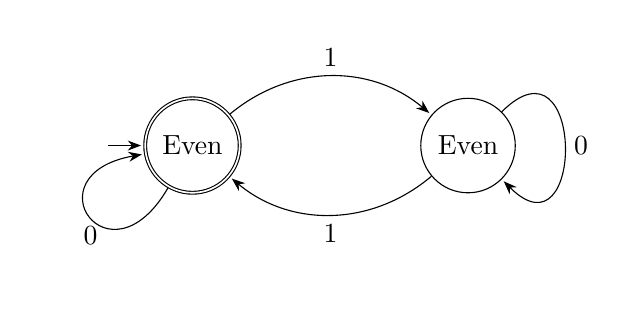
\begin{tikzpicture}[
        shorten >=1pt, 
        node distance=3.5cm, 
        on grid, 
        auto,
        >=Stealth,
        % Styling the initial arrow to match the clean blocky arrow style
        initial text={},
        every state/.style={minimum size=1.2cm}
    ]

    % --- State Definitions ---
    % Left state: Initial and Accepting (double circle)
    \node[state, initial, accepting] (s0) {Even};
    
    % Right state: Regular state
    \node[state, right=of s0] (s1) {Even};

    % --- Transitions and Loops ---
    \path[->] 
        % Loops on 0
        (s0) edge [loop below, min distance=1.5cm, out=240, in=190] node {0} (s0)
        (s1) edge [loop right, min distance=1.5cm, out=45, in=315] node {0} (s1)
        
        % Alternating transitions on 1
        (s0) edge [bend left=40] node {1} (s1)
        (s1) edge [bend left=40] node {1} (s0);

    \end{tikzpicture}
\end{center}
\mk{10} \yr{CSE 105 | L-1/T-2 | 2011--12}


%% Q21 — 2013-14
\item Explain the bitwise right-shift operator. Write a program that takes an integer $x$ as input and outputs how many \texttt{'0'}s are at the end of the binary representation of $x!$ (factorial of $x$). Assume 64-bit integers and that $x!$ will not exceed the integer boundary.
\mk{15} \yr{CSE 105 | L-1/T-2 | 2010--11}

%% Q19 — 2012-13
\item Give definitions for the following functions using bitwise operators:
\begin{enumerate}
  \item \texttt{unsigned bw\_get(unsigned x, int p, int n);} \quad returns the right-adjusted $n$ bits of \texttt{x} beginning at position \texttt{p}.
  \item \texttt{unsigned bw\_set(unsigned x, int p, int n, unsigned y);} \quad returns \texttt{x} with the right-adjusted $n$ bits beginning at position \texttt{p} set to the rightmost $n$ bits of \texttt{y}, all other bits unchanged.
\end{enumerate}
You may assume only valid values will be passed for \texttt{p} and \texttt{n}.
\mk{10} \yr{CSE 101 | L-1/T-2 | 2008--09}

%% Q18 — 2010-11
\item Write a function \texttt{int XOR(int x, int y, int p, int n)} that takes \texttt{n} bits of \texttt{y} starting at position \texttt{p}, performs bitwise XOR with the \texttt{n} bits of \texttt{x} starting at position \texttt{p}, leaves all remaining bits unchanged, and returns the result. Assume LSB is at position 0.
\mk{10} \yr{CSE 105 | L-1/T-2 | 2007--08}

%% Q16 — 2007-08
\item In a two's-complement system, \texttt{x \&= (x-1)} deletes the rightmost 1-bit in \texttt{x}. Explain why. Use this observation to write a function \texttt{int bitcount(int x)} that efficiently counts the number of 1-bits in \texttt{x}.
\mk{10} \yr{CSE 105 | L-1/T-2 | 2007--08}

%% Q17 — 2008-09
\item Invert the middle 4 bits (bit numbers 2 to 5) of a 1-byte character variable using bitwise operators. Here, inversion means converting a bit from 0 to 1 and vice versa.
\mk{10} \yr{CSE 105 | L-1/T-2 | 2005--06}

%% Q15 — 2007-08
\item Suppose \texttt{ch} is a \texttt{char} variable. Using bitwise operations only, determine whether the value stored in \texttt{ch} is positive or negative.
\mk{7} \yr{CSE 101N | L-1/T-1 | 2003--04}

%% Q12 — 2003-04
\item Write appropriate bitwise expressions that will:
\begin{enumerate}
  \item Place 1s in the \textbf{even} bit locations (bits 0, 2, 4, \ldots, 14) of a 16-bit unsigned integer \texttt{v}, leaving the odd bits unchanged.
  \item Toggle (invert) bits 1 and 6 of a 16-bit unsigned integer \texttt{v} while preserving all remaining bits.
\end{enumerate}
\mk{5} \yr{CSE 101N | L-1/T-1 | 2003--04}


%% Q14 — 2005-06
\end{enumerate}

%%──────────────────────────────────────────────────────────────────────
%% ── S9: Preprocessors, Variable Arguments & Error Handling ───────────
\section{S9 --- Preprocessors, Var-Arg \& Error Handling}
\label{sec:S9}
\markboth{S9 --- Preprocessors, Var-Arg \& Error Handling}{}

%%──────────────────────────────────────────────────────────────────────
\subtopic{cD}{Header Files \& Preprocessors}
\label{sub:s9-preproc}

\begin{enumerate}

\item Define a macro swap(d, t, x, y) where t is the name of a temporary variable, the values of x and y will be swapped, and d is the data type of the three variable. Use this macro in main to swap values of two variables. Output the values of the variables before and after swapping.
\mk{7} \yr{CSE 101 | L-1/T-1 | 2024--25}
   

%% Q7 — 2023-24
\item Consider the following two definitions of the same macro:
 
\begin{lstlisting}
#define square_1(x)   x*x
#define square_2(x)   (x)*(x)
\end{lstlisting}
Give an example where these two macros behave differently, and explain why \texttt{square\_2} is probably a better definition.
\mk{5} \yr{CSE 101 | L-1/T-1 | 2023--24}

%% Q8 — 2003-04
\item The following program contains macro-related bugs. Provide the output of the program as written, then make the necessary corrections (write only the corrected lines):
 
\begin{lstlisting}
#define cube(a) a * a * a;
#define swap(t, x, y) t=x; x=y; y=t;
#define max(x, y) x > y? x: y;
int main() {
    int a = 10, b = 20, t = 0;
    if (a > b) swap(t, a, b);
    printf("%d %d\n", a, b);
    int c = cube(b + 2);
    printf("%d\n", c);
    int max_val = max(a++, b++);
    printf("%d %d %d\n", a, b, max_val);
    return 0;
}
\end{lstlisting}
\mk{12} \yr{CSE 101 | L-1/T-1 | 2021--22}

\item Suppose we have defined two macros SQ \& CUB like below:

\begin{lstlisting}[language=C, basicstyle=\ttfamily, frame=none]
#define SQ(x) ((x)*(x))
#define CUB(x) (SQ(x)*(x))
\end{lstlisting}

\vspace{0.5em}
\noindent
Define a third macro \textit{F\_POW(x)} using the above two macros in your definition that will produce:

\[
\frac{x^3}{x^8}
\]\mk{5} \yr{CSE 101 | L-1/T-1 | 2020--21}

%% Q30 — 2021-22
\item Find a scenario where the macro \texttt{\#define SQ(x) ((x) * (x))} leads to a compilation error.
\mk{5} \yr{CSE 101 | L-1/T-1 | 2018--19}

%% Q28 — 2018-19
\item Given macros \texttt{\#define SQ(x) ((x)*(x))} and \texttt{\#define CUBE(x) (SQ(x)*(x))}, define a third macro \texttt{F\_POW(x)} using these two that computes $x^{3/4}$.
 
\mk{5} \yr{CSE 101 | L-1/T-1 | 2018--19}

%% Q29 — 2020-21
\item Write a C preprocessor macro \texttt{min3(a, b, c)} that finds the minimum of \texttt{a}, \texttt{b}, and \texttt{c}. Then write \texttt{min4(a, b, c, d)} that finds the minimum of four values using \texttt{min3}.
\mk{7} \yr{CSE 101 | L-1/T-1 | 2015--16}

%% Q26 — 2015-16 [Backlog]
\item Discuss the problems and solutions for the following parameterised macros:
\begin{enumerate}
  \item \texttt{\#define square(x) x*x}
  \item \texttt{\#define swap(t,x,y) t = x; x = y; y = t;}
  \item \texttt{\#define swap(t,x,y) \{t = x; x = y; y = t;\}}
\end{enumerate}
 
\mk{9} \yr{CSE 101 | L-1/T-1 | 2015--16}

%% Q27 — 2018-19
\item Consider the following code where the macro \texttt{abs} is intended to return the absolute value of its parameter:
 
\begin{lstlisting}
#include <stdio.h>
#define abs(x) (x < 0 ? -x : x)
int x;
int doubleGlobalX() { x *= 2; return x; }
int main() {
    scanf("%d", &x);
    printf("%d\n", abs(doubleGlobalX()));
    return 0;
}
\end{lstlisting}
What will be the output when the user inputs $-5$ and then $5$? Explain your answer.
\mk{5} \yr{CSE 105 | L-1/T-2 | 2014--15}

%% Q25 — 2015-16
\item Write a preprocessor macro \texttt{pyramid(n)} that prints a number pyramid with $n$ rows as shown below (e.g.\ for $n=3$: row 1 prints \texttt{1}; row 2 prints \texttt{212}; row 3 prints \texttt{32123}). Why is a preprocessor faster than a function call?
\begin{center}
  \begin{tabular}{|C{2cm}|C{2cm}|C{2.5cm}|}
\hline
\textbf{For n = 3} & \textbf{For n = 4} & \textbf{For n = 5} \\ \hline
1      & 1        & 1          \\ 
212    & 212      & 212        \\ 
32123  & 32123    & 32123      \\ 
       & 4321234  & 4321234    \\ 
       &          & 543212345  \\ \hline
\end{tabular}
\end{center}

\mk{8} \yr{CSE 105 | L-1/T-2 | 2013--14}

%% Q22 — 2013-14
\item Consider the two macro definitions:
 
\begin{lstlisting}
#define square_1(x) x * x
#define square_2(x) (x)*(x)
\end{lstlisting}
Give an example where they behave differently, and explain why \texttt{square\_2} is the better definition.
\mk{8} \yr{CSE 105 | L-1/T-2 | 2013--14}

%% Q23 — 2013-14
\item Consider the macro \texttt{\#define max(a, b) ((a) > (b) ? (a) : (b))}. What problem arises when executing \texttt{int z = max(i++, j++);}? Redefine the macro so that this problem does not exist. Assume the macro is applied only to integers.
 
\mk{8} \yr{CSE 105 | L-1/T-2 | 2013--14}

%% Q24 — 2014-15
\item Write preprocessor directives for the following: if \texttt{flag} is 0, define \texttt{COLOR} as 1; if \texttt{flag} is less than 3 (but nonzero), define \texttt{COLOR} as 2; if \texttt{flag} is 3 or more, define \texttt{COLOR} as 3.
\mk{5} \yr{CSE 105 | L-1/T-2 | 2012--13}

%% Q20 — 2012-13
\item Replace the following code block by defining a macro \texttt{display(i)} and using a \texttt{for} loop:
 
\begin{lstlisting}
printf("x1 = %f\n", x1);
printf("x2 = %f\n", x2);
/* ... */
printf("x10 = %f\n", x10);
\end{lstlisting}
\mk{5} \yr{CSE 105 | L-1/T-2 | 2012--13}

%% Q21 — 2013-14
\item What could be the problem with the following macro definition?
 
\begin{lstlisting}
#define SQUARE(x) x * x
\end{lstlisting}
\mk{6} \yr{CSE 105 | L-1/T-2 | 2011--12}

%% Q19 — 2012-13
\item Define a macro and write a macro in C to swap two data items.
\mk{5} \yr{CSE 105 | L-1/T-2 | 2010--11}

%% Q15 — 2010-11
\item What are the advantages and disadvantages of using a macro over a function?
\mk{8} \yr{CSE 105 | L-1/T-2 | 2010--11}

%% Q16 — 2010-11
\item Write the definition of a macro \texttt{CUBE(x)} that computes the cube of \texttt{x} so that the following statements all evaluate correctly:
\begin{lstlisting}
int x, y, z;
x = CUBE(-5);
y = CUBE(4-1);
z = !CUBE(3);
\end{lstlisting}
 
\mk{6} \yr{CSE 105 | L-1/T-2 | 2010--11}

%% Q17 — 2010-11
\item Briefly show the uses of the following library functions with example programs:
\begin{enumerate}
  \item \texttt{malloc} defined in \texttt{stdlib.h}
  \item \texttt{atoi} defined in \texttt{stdlib.h}
  \item \texttt{strcmp} defined in \texttt{string.h}
\end{enumerate}
\mk{9} \yr{CSE 105 | L-1/T-2 | 2010--11}

%% Q18 — 2011-12
\item What is macro substitution? Describe its benefits.
\mk{10} \yr{CSE 105 | L-1/T-2 | 2007--08}

%% Q13 — 2007-08
\item Write a macro \texttt{MAX(X, Y)} that finds the maximum of \texttt{X} and \texttt{Y}. Write another macro \texttt{MAX3(X, Y, Z)} that finds the maximum of \texttt{X}, \texttt{Y}, and \texttt{Z} by using \texttt{MAX(X, Y)}.
\mk{10} \yr{CSE 105 | L-1/T-2 | 2007--08}

%% Q14 — 2010-11
\item What are the differences between a function and a macro? Write a macro for computing the maximum of 3 numbers, where these 3 numbers are given as arguments.
\mk{5} \yr{CSE 105 | L-1/T-2 | 2005--06}

%% Q11 — 2005-06
\item Most C programs start with :
\begin{lstlisting}
  #include <stdio.h>
\end{lstlisting}
Why is it necessary? How does the compiler deal with this type of statement?
\mk{7} \yr{CSE 105 | L-1/T-2 | 2005--06}

%% Q12 — 2007-08
\item What is the main advantage of using macros? How is a multiline macro defined in C?
\mk{5} \yr{CSE 101N | L-1/T-1 | 2003--04}

%% Q9 — 2003-04
\item What are two different ways to define integer constants in C?
\mk{3} \yr{CSE 101N | L-1/T-1 | 2003--04}

%% Q10 — 2005-06
\end{enumerate}

%%──────────────────────────────────────────────────────────────────────
\subtopic{cD}{Variable Argument Functions}
\label{sub:s9-vararg}

\begin{enumerate}


\item Write a function where the first parameters is a string. The string may contain multiple specifiers "\%d". The subsequent parameters will be integers as specified in the string. The function will print the string by replacing the specifiers with the corresponding integers (subsequent parameters).
\mk{12}  \yr{CSE 101 | L-1/T-1 | 2024--25}


%% Q5 — 2009-10
\item Write the required function for the given program so that the main function runs correctly. The required function takes one integer and a string as fixed arguments and then a variable number of arguments. The first argument denotes the total number of lists, and the second argument denotes the format of each list. Note all the lists have the same format. Each list element can be a character, an int, or a string. The format string consists of character 's' which denotes the string element, 'i' which denotes the integer element, and 'c' which denotes the character element. The function will return the summation of all elements of all lists. The value of the string element is the summation of the ASCII values of all character.
\begin{lstlisting}
#include <stdio.h>
#include <stdarg.h>
#include <string.h>


// you cannot change the main function
int main() {
    int total_sum = getTotalSum(2, "sicc", "I am confident", 
        2, 'p', 'a', "I will pass", 3, 'p', 'b');
    // first argument "2" means 2 lists
    // second agreement "sicc" means each list has a total 
    // of 4 elements. The first element is a string, the 
    // second element is an integer, the third element is a 
    // character, and the fourth element is a character.
    // Then a total of 8 arguments are passed as 2 lists 
    // each having 4 elements requiring 8 arguments
    printf("%d\n", total_sum); // prints 2737
    total_sum = getTotalSum(2, "ic", 10, 'A', 20, 'a');
    printf("%d\n", total_sum); // prints 192 (10 + 65 + 20 + 97)
    return 0;
}
\end{lstlisting}
\mk{10} \yr{CSE 101 | L-1/T-1 | 2021--22}

\item Write a function \texttt{isPrime} that takes a variable number of inputs and returns the total count of prime numbers among them. The first argument specifies the total number of variable arguments. For example, \texttt{isPrime(6, 3, 7, 9, 11, 15, 20)} returns 3 because 3, 7, and 11 are prime.
\mk{10} \yr{CSE 101 | L-1/T-1 | 2015--16}

%% Q10 — 2021-22
\item Implement a function \texttt{void printPoint(int n, ...)} that prints the integer coordinates of a point in an $n$-dimensional space. For example, \texttt{printPoint(2, 5, 3)} prints the 2D point $(5,3)$, and \texttt{printPoint(3, 10, 7, 8)} prints the 3D point $(10,7,8)$.
\mk{10} \yr{CSE 105 | L-1/T-2 | 2014--15}

%% Q9 — 2015-16
\item The function \textbf{\textit{putInt(int var)}} accepts one argument and displays the value of \textit{var} on monitor screen. There are total three functions of similar kind that displays three data types named integer, float and character. The argument \textit{var} contains a value to be displayed. For an instance, the program code ``\textbf{\textit{putChar(char c)}}'' displays the value of c on monitor screen, where c is of character type. Similarly, \textbf{\textit{putFloat(float x)}} will display value of x on monitor screen with two digits after the decimal point.

\noindent Using any of the above functions, write a C functions \textbf{\textit{print(const char *str,...)}} that will accept a \textit{format} string and a number of variables, and then will display the contents of the variables on monitor screen.

\vspace{0.3cm}
\noindent Some sample input and output are given below--

\begin{center}
\begin{tabular}{|l|l|}
\hline
\textbf{Sample input} & \textbf{Sample output} \\ \hline
print("\%d", A); & 12 \\ \hline
print("\%c \%f \%d", ch, x, A); & P 12.34 40 \\ \hline
print("\%d \%d \%f \%c", A, B, X, ch); & 23 11 45.23 D \\ \hline
\end{tabular}
\end{center} 

\mk{20} \yr{CSE 105 | L-1/T-2 | 2013--14}

%% Q8 — 2014-15
\item Write a C function with prototype \texttt{double avgPrice(const char *str, ...)} that calculates the average price of all books listed as \texttt{<name, price>} pairs in a variable argument list, terminated by \texttt{NULL}. For example:
\begin{lstlisting}
avg = avgPrice("book list", "mathematics", 12.75,
               "programming with C", 20.75,
               "physics", 23.20, NULL);
\end{lstlisting}
\mk{10} \yr{CSE 105 | L-1/T-2 | 2012--13}

%% Q7 — 2013-14
\item Implement \texttt{int printf(char *str, ...)} as defined in \texttt{stdio.h} using the variable argument passing technique.
\mk{15} \yr{CSE 101 | L-1/T-2 | 2009--10}

%% Q6 — 2012-13
\end{enumerate}

%%──────────────────────────────────────────────────────────────────────
\subtopic{cD}{Error Handling}
\label{sub:s9-error}

\begin{enumerate}

%% Q6 — 2007-08
\item Identify all the problems in the following code segment:
 
\begin{lstlisting}
int main() {
    int a;
    int diff;
    int *q;
    double *p;
    a = 10;
    p = &a;      /* line 8  */
    *p = 100;    /* line 9  */
    *q = 10;     /* line 10 */
    p = p + 2;   /* line 11 */
    p = p - 2;   /* line 12 */
    p = p * 1;   /* line 13 */
    p = p / 1;   /* line 14 */
    diff = p - q;/* line 15 */
    return 0;
}
\end{lstlisting}
\mk{6} \yr{CSE 101 | L-1/T-1 | 2015--16}

\item Write a C program to solve the quadratic equation $ax^2 + bx + c = 0$, where $a$, $b$, and $c$ are constants taken as inputs. Include all necessary error-handling code. Output imaginary roots in the form $p + iq$ where $i^2 = -1$.
\mk{10} \yr{CSE 101 | L-1/T-2 | 2008--09}

%% Q8 — 2015-16
\item A compiler error is reported for the following code segment. What is the possible error? Also describe the way(s) to fix it.
 
\begin{lstlisting}
void test() {
    a = 20;
}
int a;
void main() {}
\end{lstlisting}
\mk{5} \yr{CSE 105 | L-1/T-2 | 2007--08}

%% Q7 — 2008-09
\end{enumerate}

%% ══════════════════════════════════════════════════════════════════════
%%  PART V — DATA STRUCTURES
%% ══════════════════════════════════════════════════════════════════════
\secdivider{Part V}{Data Structures}{cE}{cE}

%% ── S10: Abstract Data Structures ────────────────────────────────────
\section{S10 --- Abstract Data Structures}
\label{sec:S10}
\markboth{S10 --- Abstract Data Structures}{}
{\small\textcolor{cE}{\textit{Note: The following questions appeared in past CSE 105 and CSE 101 papers but fall \textbf{outside} the CSE101 syllabus. Included for reference only.}}
\vspace{4pt}}

%%──────────────────────────────────────────────────────────────────────
\subtopic{cE}{Linked Lists}
\label{sub:s10-linkedlist}

\begin{enumerate}

%% Q1 — 2005-06
\item What is a doubly linked list? Define the structure of a node in a doubly linked list where each node stores two integer variables and one character variable.
\mk{10} \yr{CSE 105 | L-1/T-2 | 2011--12}

%% Q8 — 2011-12
\item A doubly linked list uses a type \texttt{DLL} (defined via \texttt{typedef}) where each node has an integer \texttt{data}, a \texttt{next} pointer, and a \texttt{prev} pointer. The function \texttt{findNode(DLL *pHead, int target)} is given (it returns \texttt{pCur->next} if found, or \texttt{NULL}). Write the following two functions which \textbf{must} use \texttt{findNode()} to locate the target node:
\begin{enumerate}
  \item \texttt{int deleteNode(DLL **pHead, int target);} --- deletes the node with \texttt{data == target}; returns 1 if deleted, 0 if not found.
  \item \texttt{int insertNode(DLL **pHead, int target, int newData);} --- inserts a new node with \texttt{newData} after the node with \texttt{data == target}; returns 1 if inserted, 0 if target not found.
\end{enumerate}
\begin{lstlisting}
  DLL* findNode(DLL* pHead, int target){
    DLL* pCur;
    //Search the nodes in a linked list
    pCur=pHead;
    //Search until the target value is found or the end of the list is reached
    while(pCur!=NULL && pCur->data!=target){
      pCur=pCur->next;
    }
    if(pCur!=NULL){
      return pCur->next;
    }else{
      return NULL;
    }
  }
\end{lstlisting}
\mk{20} \yr{CSE 105 | L-1/T-2 | 2011--12}

%% Q9 — 2011-12
\item Assume the doubly linked list above is sorted in ascending order of \texttt{data}. Write \texttt{insertNode1()} such that if \texttt{insertNode()} returns 0 (target not found), it finds the node with the predecessor value of \texttt{target} and inserts the new node after it.
\mk{5} \yr{CSE 105 | L-1/T-2 | 2011--12}

\item Consider the following structure for a singly linked list:
\begin{lstlisting}
struct Node { int val; struct Node *next; };
\end{lstlisting}
\begin{enumerate}
  \item Write an \texttt{insert} function that inserts elements in ascending sorted order. Prototype: \texttt{struct Node *insert(struct Node *head, int val);}. The function searches for the correct position, allocates a new node, inserts it, and returns the (possibly new) head.
  \item Write a recursive function \texttt{void print(struct Node *elem)} that prints the linked list in reverse order.
\end{enumerate}
\mk{23} \yr{CSE 105 | L-1/T-2 | 2010--11}

%% Q6 — 2010-11
\item What are the advantages and disadvantages of using a linked list over arrays?
\mk{8} \yr{CSE 105 | L-1/T-2 | 2010--11}

%% Q7 — 2011-12
\item Define a self-referential structure containing the following members:
\begin{enumerate}
  \item A 40-element character array \texttt{name} and a 15-element character array \texttt{std\_id}.
  \item A date-type member \texttt{DOB} containing \texttt{day} (1--31), \texttt{month} (1--12), and \texttt{year} (1900--2100).
  \item Variables \texttt{m\_mark} and \texttt{p\_mark} for marks (0--100) in math and physics respectively; \texttt{m\_total} holds their sum.
  \item A pointer \texttt{next} to another structure of this same type.
\end{enumerate}

Write a C function to create a linked list for storing students' information (using the self-referential structure with name, student ID, date of birth, physics mark, math mark, and a \texttt{next} pointer).
\mk{15} \yr{CSE 101 | L-1/T-2 | 2008--09}

%% Q4 — 2008-09
\item Suppose you have a one-way linked list where each node stores \texttt{name} (\texttt{char *}) and \texttt{age} (\texttt{short int}). Write two functions:
\begin{enumerate}
  \item \texttt{void ll\_to\_file(char *file\_name, node *head);}
  \item \texttt{node *ll\_from\_file(char *file\_name);}
\end{enumerate}
that store and retrieve the entire linked list to/from a file, preserving node order.
\mk{25} \yr{CSE 101 | L-1/T-2 | 2008--09}

%% Q5 — 2010-11
\item How can you define a linked list in a C program? Compare a linked list with an array.
\mk{10} \yr{CSE 105 | L-1/T-2 | 2005--06}

%% Q2 — 2005-06
\item Describe, with C code, the different cases that may arise during insertion of a node into a linked list. How can you insert a new node into a sorted linked list while maintaining the sorted order?
\mk{25} \yr{CSE 105 | L-1/T-2 | 2005--06}

%% Q13 — 2003-04
\item When does a linked list have superior utility over an array?
\mk{4} \yr{CSE 101N | L-1/T-1 | 2003--04}

%% Q14 — 2003-04
\item Write a function \texttt{void deleteNodes(Node *p, Node *q)} that deletes all nodes from just after \texttt{p} up to and including \texttt{q} from a singly linked list, adjusting the \texttt{next} pointers accordingly and freeing all deleted nodes. Assume \texttt{p} is to the left of \texttt{q} and neither is \texttt{NULL}.

\begin{center}
  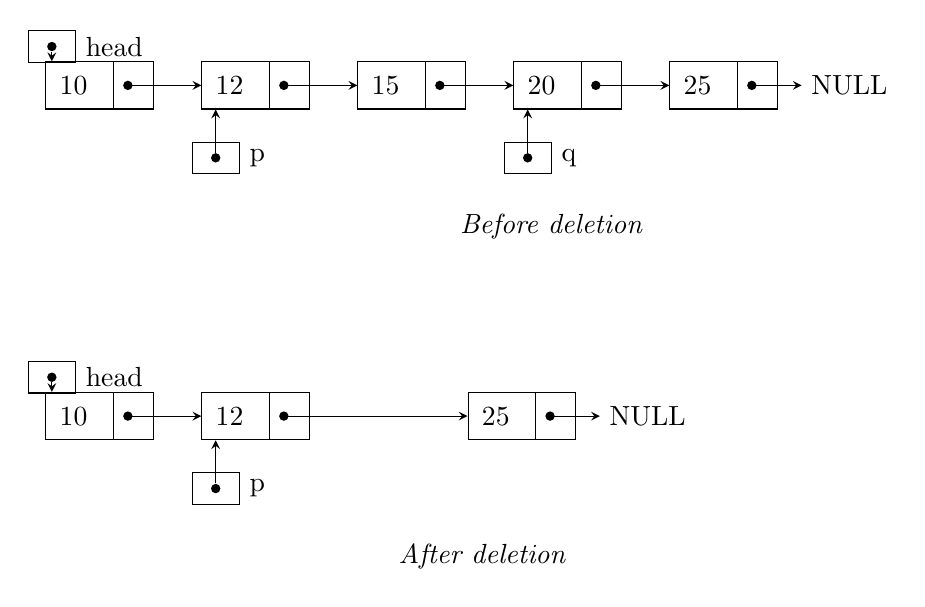
\begin{tikzpicture}[
    listnode/.style={
        rectangle split, 
        rectangle split parts=2, 
        draw, 
        rectangle split horizontal,
        inner sep=5pt,
        minimum height=0.6cm
    },
    ptrbox/.style={
        draw, 
        minimum width=0.6cm, 
        minimum height=0.4cm
    },
    dot/.style={
        fill=black,
        circle,
        inner sep=1.2pt
    },
    >=stealth
]

% ==========================================
% BEFORE DELETION
% ==========================================

% Nodes
\node[listnode] (n1) {\makebox[0.5cm][l]{10} \nodepart{two} \makebox[0.15cm]{}};
\node[listnode, right=0.6cm of n1] (n2) {\makebox[0.5cm][l]{12} \nodepart{two} \makebox[0.15cm]{}};
\node[listnode, right=0.6cm of n2] (n3) {\makebox[0.5cm][l]{15} \nodepart{two} \makebox[0.15cm]{}};
\node[listnode, right=0.6cm of n3] (n4) {\makebox[0.5cm][l]{20} \nodepart{two} \makebox[0.15cm]{}};
\node[listnode, right=0.6cm of n4] (n5) {\makebox[0.5cm][l]{25} \nodepart{two} \makebox[0.15cm]{}};

% Pointers (Dots inside node partitions)
\node[dot] at (n1.two) {};
\node[dot] at (n2.two) {};
\node[dot] at (n3.two) {};
\node[dot] at (n4.two) {};
\node[dot] at (n5.two) {};

% Connecting Arrows
\draw[->] (n1.two) -- (n2.west);
\draw[->] (n2.two) -- (n3.west);
\draw[->] (n3.two) -- (n4.west);
\draw[->] (n4.two) -- (n5.west);

\node[right=0.3cm of n5] (null1) {NULL};
\draw[->] (n5.two) -- (null1);

% Head Pointer
\node[ptrbox, above=0.4cm of n1.one, anchor=south, xshift=-0.1cm] (head) {};
\node[right=0cm of head] {head};
\node[dot] (headdot) at (head.center) {};
\draw[->] (headdot) -- (headdot |- n1.north);

% p Pointer
\node[ptrbox, below=0.6cm of n2.one, anchor=north] (p) {};
\node[right=0cm of p] {p};
\node[dot] (pdot) at (p.center) {};
\draw[->] (pdot) -- (pdot |- n2.south);

% q Pointer
\node[ptrbox, below=0.6cm of n4.one, anchor=north] (q) {};
\node[right=0cm of q] {q};
\node[dot] (qdot) at (q.center) {};
\draw[->] (qdot) -- (qdot |- n4.south);

% Section Label
\node[below right=1.2cm and -0.2cm of n3] {\textit{Before deletion}};


% ==========================================
% AFTER DELETION
% ==========================================
\begin{scope}[yshift=-4.2cm]

    % Nodes
    \node[listnode] (m1) {\makebox[0.5cm][l]{10} \nodepart{two} \makebox[0.15cm]{}};
    \node[listnode, right=0.6cm of m1] (m2) {\makebox[0.5cm][l]{12} \nodepart{two} \makebox[0.15cm]{}};
    % Shift node 25 to accurately reflect the visual gap left by the deleted nodes
    \node[listnode, right=2cm of m2] (m5) {\makebox[0.5cm][l]{25} \nodepart{two} \makebox[0.15cm]{}};

    % Pointers (Dots inside node partitions)
    \node[dot] at (m1.two) {};
    \node[dot] at (m2.two) {};
    \node[dot] at (m5.two) {};

    % Connecting Arrows
    \draw[->] (m1.two) -- (m2.west);
    \draw[->] (m2.two) -- (m5.west);
    
    \node[right=0.3cm of m5] (null2) {NULL};
    \draw[->] (m5.two) -- (null2);

    % Head Pointer
    \node[ptrbox, above=0.4cm of m1.one, anchor=south, xshift=-0.1cm] (head2) {};
    \node[right=0cm of head2] {head};
    \node[dot] (headdot2) at (head2.center) {};
    \draw[->] (headdot2) -- (headdot2 |- m1.north);

    % p Pointer
    \node[ptrbox, below=0.6cm of m2.one, anchor=north] (p2) {};
    \node[right=0cm of p2] {p};
    \node[dot] (pdot2) at (p2.center) {};
    \draw[->] (pdot2) -- (pdot2 |- m2.south);

    % Section Label
    \node[below right=1.2cm and 1cm of m2] {\textit{After deletion}};

\end{scope}

\end{tikzpicture}
\end{center}

\mk{10} \yr{CSE 101N | L-1/T-1 | 2003--04}

%% Q3 — 2008-09
\end{enumerate}

%%──────────────────────────────────────────────────────────────────────
\subtopic{cE}{Stacks \& Queues}
\label{sub:s10-stackqueue}

\begin{enumerate}
  %% Q18 — 2008-09
\item Write down a generic implementation (\texttt{init}, \texttt{push}, \texttt{pop}) of a stack that can be used with any datatype. Implement the stack as an array of \texttt{void} pointers (capacity 500). The \texttt{push} function should take the size of the data as an argument and allocate necessary memory. Use:
\begin{lstlisting}
void *memcpy(void *dest, void *src, int n);
\end{lstlisting}
The \texttt{pop} function should free any memory previously allocated by \texttt{push}.
\mk{13} \yr{CSE 101 | L-1/T-2 | 2008--09}

\item Implement a queue for integer variables. There is an array \texttt{queue} of 100 integers. Write two functions:
\begin{enumerate}
  \item \texttt{void enqueue(int i)} --- inserts \texttt{i} at the last position of existing elements.
  \item \texttt{int dequeue()} --- retrieves the front element.
\end{enumerate}
Assume other necessary variables so that the FIFO property is maintained.
\mk{15} \yr{CSE 105 | L-1/T-2 | 2007--08}

%% Q2 — 2008-09
\end{enumerate}

%%──────────────────────────────────────────────────────────────────────
\subtopic{cE}{Binary Search Trees}
\label{sub:s10-bst}

\begin{enumerate}

  \item  A tree has exactly one path from the root (e.g., the node marked with 8 in the Figure is the root) to any node. A binary tree is a tree where each node has at most two children. For example, node 3 and node 10 are the children of node 8; similarly, node 1 and node 6 are the children of node 3. Moreover, node 3 is the left child and node 10 is the right child of node 8. Also note that, nodes 1, 3, 4, 6 and 7 are in the left subtree and nodes 10, 13 and 14 are in the right subtree of node 8.
\begin{center}
  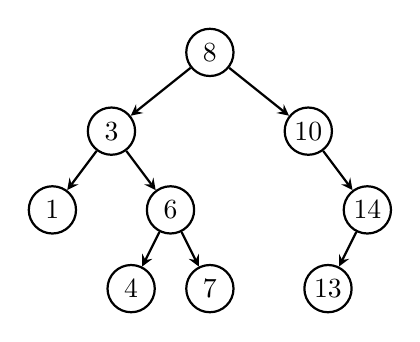
\begin{tikzpicture}[
        every node/.style={circle, draw, thick, minimum size=6mm, inner sep=0pt},
        level 1/.style={sibling distance=25mm, level distance=10mm},
        level 2/.style={sibling distance=15mm, level distance=10mm},
        level 3/.style={sibling distance=10mm, level distance=10mm},
        edge from parent/.style={draw, ->, thick, >=stealth}
    ]
    \node {8}
        child {node {3}
            child {node {1}}
            child {node {6}
                child {node {4}}
                child {node {7}}
            }
        }
        child {node {10}
            child[missing]
            child {node {14}
                child {node {13}}
                child[missing]
            }
        };
    \end{tikzpicture}
\end{center}
\noindent
A binary search tree is a binary tree where the value of each node in the left subtree of a node is smaller than the value of that node, while the value of each node in the right subtree is equal to or higher than the value of that node. A binary search tree is represented by a 1D array as follows--

\begin{itemize}
    \item[(i)] The root is placed at index 1.
    \item[(ii)] If a node is in index $i$, then its left child is placed at index $2i$ and the right child is placed at index $2i + 1$.
    \item[(iii)] -1 indicates the node does not exist.
\end{itemize}

\noindent
Write a recursive C function that will generate a binary search tree from some given values by inserting one value at a time using the following function prototype--

\begin{lstlisting}
int insertNode(int *tree, int x);
// x will be inserted into tree as a node.
\end{lstlisting}

\noindent
Also write a recursive C function that counts the number of nodes available in the tree.
\mk{13} \yr{CSE 101 | L-1/T-1 | 2020--21}

%% Q19 — 2021-22
\item
  \begin{enumerate}
    \item A binary expression tree is a specific kind of a binary tree used to represent
    expressions. The leaves of the binary expression tree are operands, such as constants or
    variable names, and the other nodes contain operators. Assume the set of possible
    operators are \{`+', `-', `*', `/'\}. The set of possible operands are [`0'-`9']. See the figure
    below, which is the binary expression tree for the expression (in in-fix notations):
    $(((2+3)*9)+7)$

    \begin{figure}[h]
      \centering
      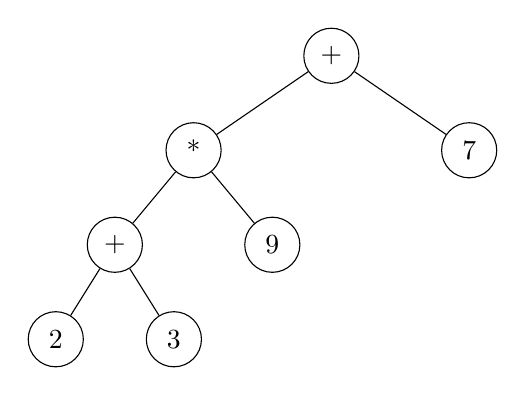
\begin{tikzpicture}[
        every node/.style={circle, draw, minimum size=7mm},
        level distance=1.2cm,
        level 1/.style={sibling distance=3.5cm},
        level 2/.style={sibling distance=2cm},
        level 3/.style={sibling distance=1.5cm}
      ]
        \node {+}
          child { node {*}
            child { node {+}
              child { node {2} }
              child { node {3} }
            }
            child { node {9} }
          }
          child { node {7} };
      \end{tikzpicture}
    \end{figure}

    The input contains several lines to describe an expression tree, until the end of file. Each
    line describes a node of the tree. Such a line starts with a sequence of `L' and `R's, that
    represents the turns (left or right) you have to make to reach the node, starting from the
    root. The final character represents the content of the node -- either an operand or an
    operator. It is guaranteed that a child node's description never comes ahead of its parent
    node. Also, there are no unary operators used in the expression. For the given figure, the
    input would be:

    \begin{lstlisting}
+
L*
R7
LL+
LR9
LLL2
LLR3
    \end{lstlisting}

    Given description of a particular binary expression tree, you need to construct it using
    self referential data structure (i.e. a structure definition which includes at least one
    member that is a pointer to the structure of its own kind). Store the root of the tree in a
    local variable called \texttt{root}.

    \textbf{Do not use global variables.} \mk{20}

    \item Postfix notation is a mathematical notation in which every operator follows all of its
    operands. An expression in postfix notation is parenthesis-free. For example, for the infix
    expression $(((2+3)*9)+7)$, the expression in postfix notation is: \texttt{2 3 + 9 * 7 +}.
    Using the expression tree, constructed in 8(a) and represented by the variable \texttt{root}, write necessary
    code to produce the expression in postfix notation. There should be a space printed after
    printing each operator/operand.\mk{10}
  \end{enumerate} 
 \yr{CSE 105 | L-1/T-2 | 2014--15}



%% Q1 — 2007-08
\item A BST is stored in a 1-D array where the root is at index 1; the left and right children of \texttt{node[i]} are at \texttt{node[2*i]} and \texttt{node[2*i+1]}; value $-1$ means no element.
\begin{enumerate}
  \item Write a recursive C function \texttt{void BST\_insert(int node[], int x)} that inserts element \texttt{x} into the BST. If the tree is empty, \texttt{x} becomes the root.
  \item Write a recursive C function that returns the height of a given node (root has height 0; a non-existent node has height $-1$).
\end{enumerate}
\mk{20} \yr{CSE 105 | L-1/T-2 | 2013--14}

\item A C program uses the following BST structure:
\begin{lstlisting}
typedef struct tt {
    int value;
    struct tt *lchild;
    struct tt *rchild;
} node;
node *tree;
\end{lstlisting}
For each node, all values in the left subtree are less than the node's value, and all values in the right subtree are greater. Write a C function \texttt{void insertnode(node *n)} that inserts node \texttt{n} into the tree.
 
\mk{15} \yr{CSE 105 | L-1/T-2 | 2012--13}

%% Q4 — 2011-12
\item A binary search tree is represented as a 1-D array where the root is at index 1. For a node at index $i$: its left child is at $2i$ and right child at $2i+1$. Non-existing nodes are represented by $-1$.
\begin{center}
     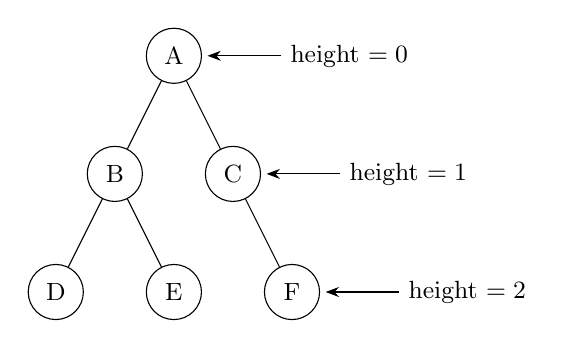
\begin{tikzpicture}[
        % Style for the tree nodes
        treenode/.style={
            draw, 
            circle, 
            minimum size=0.7cm, 
            inner sep=0pt,
            font=\small
        },
        % Style for the arrow descriptions
        height_arrow/.style={
            <-, 
            >=Stealth, 
            shorten <=2pt
        },
        % Style for individual array table cells
        tablecell/.style={
            draw,
            minimum width=0.6cm,
            minimum height=0.5cm,
            anchor=south west,
            inner sep=0pt,
            font=\small
        }
    ]

    % ==========================================
    % BINARY TREE COMPONENT
    % ==========================================
    \begin{scope}[every node/.style={treenode}]
        \node (A) at (0, 0) {A}
            child { node (B) {B} 
                child { node (D) {D} }
                child { node (E) {E} }
            }
            child { node (C) {C}
                child[missing] % Skips left child of C
                child { node (F) {F} }
            };
    \end{scope}

    % Adjusting tree layout distances cleanly
    \tikzset{level 1/.style={sibling distance=2cm, level distance=1.2cm}}
    \tikzset{level 2/.style={sibling distance=1cm, level distance=1.2cm}}

    % Height annotations and horizontal arrows
    \draw[height_arrow] (A.east) -- ++(1cm, 0) node[right, font=\small] {height $= 0$};
    \draw[height_arrow] (C.east) -- ++(1cm, 0) node[right, font=\small] {height $= 1$};
    \draw[height_arrow] (F.east) -- ++(1cm, 0) node[right, font=\small] {height $= 2$};

    \end{tikzpicture}
\end{center}
\begin{center}
  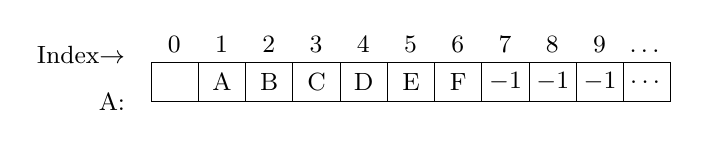
\begin{tikzpicture}[
        % Style for the tree nodes
        treenode/.style={
            draw, 
            circle, 
            minimum size=0.7cm, 
            inner sep=0pt,
            font=\small
        },
        % Style for the arrow descriptions
        height_arrow/.style={
            <-, 
            >=Stealth, 
            shorten <=2pt
        },
        % Style for individual array table cells
        tablecell/.style={
            draw,
            minimum width=0.6cm,
            minimum height=0.5cm,
            anchor=south west,
            inner sep=0pt,
            font=\small
        }
    ]

     % ==========================================
    % ARRAY TABLE COMPONENT
    % ==========================================
    \begin{scope}[yshift=-4.2cm, xshift=-2.2cm]
        % Labels on the left
        \node[left, font=\small] at (-0.2, 0.6) {Index$\rightarrow$};
        \node[left, font=\small] at (-0.2, 0) {A:};

        % Array Index Numbers (Top row)
        \node[anchor=south, font=\small] at (0.3, 0.5) {0};
        \node[anchor=south, font=\small] at (0.9, 0.5) {1};
        \node[anchor=south, font=\small] at (1.5, 0.5) {2};
        \node[anchor=south, font=\small] at (2.1, 0.5) {3};
        \node[anchor=south, font=\small] at (2.7, 0.5) {4};
        \node[anchor=south, font=\small] at (3.3, 0.5) {5};
        \node[anchor=south, font=\small] at (3.9, 0.5) {6};
        \node[anchor=south, font=\small] at (4.5, 0.5) {7};
        \node[anchor=south, font=\small] at (5.1, 0.5) {8};
        \node[anchor=south, font=\small] at (5.7, 0.5) {9};
        \node[anchor=south, font=\small] at (6.3, 0.5) {\dots};

        % Array Data Blocks (Bottom row)
        \node[tablecell] at (0, 0) {};
        \node[tablecell] at (0.6, 0) {A};
        \node[tablecell] at (1.2, 0) {B};
        \node[tablecell] at (1.8, 0) {C};
        \node[tablecell] at (2.4, 0) {D};
        \node[tablecell] at (3.0, 0) {E};
        \node[tablecell] at (3.6, 0) {F};
        \node[tablecell] at (4.2, 0) {$-1$};
        \node[tablecell] at (4.8, 0) {$-1$};
        \node[tablecell] at (5.4, 0) {$-1$};
        \node[tablecell] at (6.0, 0) {\dots};
    \end{scope}
  \end{tikzpicture}
\end{center}
\begin{enumerate}
  \item Write a C function that reads integers from standard input and places them in array \texttt{A[n]} following the 1-D BST representation principle. Assume \texttt{A[]} and \texttt{n} are declared globally.
  \item Write a C function to calculate the height of an element in the tree, where the root's height is 0. (A non-existent node has height $-1$.)
\end{enumerate}
\mk{20} \yr{CSE 101 | L-1/T-1 | 2015--16}
\yr{CSE 105 | L-1/T-2 | 2011--12}

%% Q5 — 2012-13
\item Consider a Binary Search Tree (BST) of integers. Write functions for the following tasks:
\begin{enumerate}
  \item Find the number of integers in the BST that are larger than a given integer $x$.
  \item Find the largest number in the BST.
  \item Print the numbers in the BST in descending order.
\end{enumerate}
\mk{21} \yr{CSE 101 | L-1/T-2 | 2008--09}

%% Q3 — 2011-12
\item Write C code along with the necessary data structure for:
\begin{enumerate}
  \item Building a Binary Search Tree (BST) of strings from consecutive input words.
  \item Printing the BST in lexicographically descending order.
\end{enumerate}
Draw a picture of the resulting BST if the strings are inserted in the following order:\\
``it is the best time for all good men to come to the aid of their party''.
\mk{25} \yr{CSE 105 | L-1/T-2 | 2007--08}

%% Q2 — 2008-09
\end{enumerate}

\end{document}